\documentclass[twoside]{book}

% Packages required by doxygen
\usepackage{calc}
\usepackage{doxygen}
\usepackage{graphicx}
\usepackage[utf8]{inputenc}
\usepackage{makeidx}
\usepackage{multicol}
\usepackage{multirow}
\usepackage{fixltx2e}
\PassOptionsToPackage{warn}{textcomp}
\usepackage{textcomp}
\usepackage[nointegrals]{wasysym}
\usepackage[table]{xcolor}

% Font selection
\usepackage[T1]{fontenc}
\usepackage{mathptmx}
\usepackage[scaled=.90]{helvet}
\usepackage{courier}
\usepackage{amssymb}
\usepackage{sectsty}
\renewcommand{\familydefault}{\sfdefault}
\allsectionsfont{%
  \fontseries{bc}\selectfont%
  \color{darkgray}%
}
\renewcommand{\DoxyLabelFont}{%
  \fontseries{bc}\selectfont%
  \color{darkgray}%
}
\newcommand{\+}{\discretionary{\mbox{\scriptsize$\hookleftarrow$}}{}{}}

% Page & text layout
\usepackage{geometry}
\geometry{%
  a4paper,%
  top=2.5cm,%
  bottom=2.5cm,%
  left=2.5cm,%
  right=2.5cm%
}
\tolerance=750
\hfuzz=15pt
\hbadness=750
\setlength{\emergencystretch}{15pt}
\setlength{\parindent}{0cm}
\setlength{\parskip}{0.2cm}
\makeatletter
\renewcommand{\paragraph}{%
  \@startsection{paragraph}{4}{0ex}{-1.0ex}{1.0ex}{%
    \normalfont\normalsize\bfseries\SS@parafont%
  }%
}
\renewcommand{\subparagraph}{%
  \@startsection{subparagraph}{5}{0ex}{-1.0ex}{1.0ex}{%
    \normalfont\normalsize\bfseries\SS@subparafont%
  }%
}
\makeatother

% Headers & footers
\usepackage{fancyhdr}
\pagestyle{fancyplain}
\fancyhead[LE]{\fancyplain{}{\bfseries\thepage}}
\fancyhead[CE]{\fancyplain{}{}}
\fancyhead[RE]{\fancyplain{}{\bfseries\leftmark}}
\fancyhead[LO]{\fancyplain{}{\bfseries\rightmark}}
\fancyhead[CO]{\fancyplain{}{}}
\fancyhead[RO]{\fancyplain{}{\bfseries\thepage}}
\fancyfoot[LE]{\fancyplain{}{}}
\fancyfoot[CE]{\fancyplain{}{}}
\fancyfoot[RE]{\fancyplain{}{\bfseries\scriptsize Generated on Tue May 27 2014 23\+:44\+:23 for Biometrické rozpoznávání 3\+D modelů obličeje by Doxygen }}
\fancyfoot[LO]{\fancyplain{}{\bfseries\scriptsize Generated on Tue May 27 2014 23\+:44\+:23 for Biometrické rozpoznávání 3\+D modelů obličeje by Doxygen }}
\fancyfoot[CO]{\fancyplain{}{}}
\fancyfoot[RO]{\fancyplain{}{}}
\renewcommand{\footrulewidth}{0.4pt}
\renewcommand{\chaptermark}[1]{%
  \markboth{#1}{}%
}
\renewcommand{\sectionmark}[1]{%
  \markright{\thesection\ #1}%
}

% Indices & bibliography
\usepackage{natbib}
\usepackage[titles]{tocloft}
\setcounter{tocdepth}{3}
\setcounter{secnumdepth}{5}
\makeindex

% Hyperlinks (required, but should be loaded last)
\usepackage{ifpdf}
\ifpdf
  \usepackage[pdftex,pagebackref=true]{hyperref}
\else
  \usepackage[ps2pdf,pagebackref=true]{hyperref}
\fi
\hypersetup{%
  colorlinks=true,%
  linkcolor=blue,%
  citecolor=blue,%
  unicode%
}

% Custom commands
\newcommand{\clearemptydoublepage}{%
  \newpage{\pagestyle{empty}\cleardoublepage}%
}


%===== C O N T E N T S =====

\begin{document}

% Titlepage & ToC
\hypersetup{pageanchor=false,
             bookmarks=true,
             bookmarksnumbered=true,
             pdfencoding=unicode
            }
\pagenumbering{roman}
\begin{titlepage}
\vspace*{7cm}
\begin{center}%
{\Large Biometrické rozpoznávání 3\+D modelů obličeje }\\
\vspace*{1cm}
{\large Generated by Doxygen 1.8.7}\\
\vspace*{0.5cm}
{\small Tue May 27 2014 23:44:23}\\
\end{center}
\end{titlepage}
\clearemptydoublepage
\tableofcontents
\clearemptydoublepage
\pagenumbering{arabic}
\hypersetup{pageanchor=true}

%--- Begin generated contents ---
\chapter{Hierarchical Index}
\section{Class Hierarchy}
This inheritance list is sorted roughly, but not completely, alphabetically\+:\begin{DoxyCompactList}
\item \contentsline{section}{Average\+Face}{\pageref{class_average_face}}{}
\item \contentsline{section}{Common}{\pageref{class_common}}{}
\item \contentsline{section}{Comparator}{\pageref{class_comparator}}{}
\item \contentsline{section}{Controller}{\pageref{class_controller}}{}
\item \contentsline{section}{Depth\+Map}{\pageref{class_depth_map}}{}
\item \contentsline{section}{Eigen\+Face}{\pageref{class_eigen_face}}{}
\item \contentsline{section}{Face\+Aligner}{\pageref{class_face_aligner}}{}
\item \contentsline{section}{Face\+Divider}{\pageref{class_face_divider}}{}
\item \contentsline{section}{Landmark\+Detector}{\pageref{class_landmark_detector}}{}
\item \contentsline{section}{Landmarks}{\pageref{class_landmarks}}{}
\item \contentsline{section}{Mesh}{\pageref{class_mesh}}{}
\item Q\+G\+L\+Widget\begin{DoxyCompactList}
\item \contentsline{section}{G\+L\+Widget}{\pageref{class_g_l_widget}}{}
\end{DoxyCompactList}
\item Q\+Main\+Window\begin{DoxyCompactList}
\item \contentsline{section}{Main\+Window}{\pageref{class_main_window}}{}
\end{DoxyCompactList}
\item \contentsline{section}{Run}{\pageref{class_run}}{}
\item \contentsline{section}{Score\+Fusioner}{\pageref{class_score_fusioner}}{}
\item \contentsline{section}{Score\+Normalizer}{\pageref{class_score_normalizer}}{}
\item \contentsline{section}{Stats}{\pageref{class_stats}}{}
\item \contentsline{section}{Stat\+Values}{\pageref{class_stat_values}}{}
\item \contentsline{section}{t\+Transform\+Value}{\pageref{structt_transform_value}}{}
\end{DoxyCompactList}

\chapter{Class Index}
\section{Class List}
Here are the classes, structs, unions and interfaces with brief descriptions\+:\begin{DoxyCompactList}
\item\contentsline{section}{\hyperlink{class_average_face}{Average\+Face} \\*Create average face }{\pageref{class_average_face}}{}
\item\contentsline{section}{\hyperlink{class_common}{Common} \\*This class containt static method who are used in entire project. There are constants settings for face recognition process too }{\pageref{class_common}}{}
\item\contentsline{section}{\hyperlink{class_comparator}{Comparator} \\*Class for comparation features vecters. Provide euclidian, cityblock and correlation distance }{\pageref{class_comparator}}{}
\item\contentsline{section}{\hyperlink{class_controller}{Controller} \\*Class for running batch of process }{\pageref{class_controller}}{}
\item\contentsline{section}{\hyperlink{class_depth_map}{Depth\+Map} \\*Class for create depthmap }{\pageref{class_depth_map}}{}
\item\contentsline{section}{\hyperlink{class_eigen_face}{Eigen\+Face} \\*Class for Eigenface method }{\pageref{class_eigen_face}}{}
\item\contentsline{section}{\hyperlink{class_face_aligner}{Face\+Aligner} \\*Class for align face }{\pageref{class_face_aligner}}{}
\item\contentsline{section}{\hyperlink{class_face_divider}{Face\+Divider} \\*Class for divide face to areas }{\pageref{class_face_divider}}{}
\item\contentsline{section}{\hyperlink{class_g_l_widget}{G\+L\+Widget} \\*Class for painting mesh }{\pageref{class_g_l_widget}}{}
\item\contentsline{section}{\hyperlink{class_landmark_detector}{Landmark\+Detector} \\*Class for landmark detection }{\pageref{class_landmark_detector}}{}
\item\contentsline{section}{\hyperlink{class_landmarks}{Landmarks} \\*Class for store landmarks position }{\pageref{class_landmarks}}{}
\item\contentsline{section}{\hyperlink{class_main_window}{Main\+Window} \\*Need for show up models of face }{\pageref{class_main_window}}{}
\item\contentsline{section}{\hyperlink{class_mesh}{Mesh} \\*Class for represent 3\+D model of face }{\pageref{class_mesh}}{}
\item\contentsline{section}{\hyperlink{class_run}{Run} \\*Class for running batch of process }{\pageref{class_run}}{}
\item\contentsline{section}{\hyperlink{class_score_fusioner}{Score\+Fusioner} \\*Class for score fusion }{\pageref{class_score_fusioner}}{}
\item\contentsline{section}{\hyperlink{class_score_normalizer}{Score\+Normalizer} \\*Class for score normalization }{\pageref{class_score_normalizer}}{}
\item\contentsline{section}{\hyperlink{class_stats}{Stats} \\*Class of statistacal data }{\pageref{class_stats}}{}
\item\contentsline{section}{\hyperlink{class_stat_values}{Stat\+Values} \\*Statistical values for one area face }{\pageref{class_stat_values}}{}
\item\contentsline{section}{\hyperlink{structt_transform_value}{t\+Transform\+Value} \\*Transformation values }{\pageref{structt_transform_value}}{}
\end{DoxyCompactList}

\chapter{Class Documentation}
\hypertarget{class_average_face}{\section{Average\+Face Class Reference}
\label{class_average_face}\index{Average\+Face@{Average\+Face}}
}


create average face  




{\ttfamily \#include $<$averageface.\+h$>$}

\subsection*{Public Member Functions}
\begin{DoxyCompactItemize}
\item 
\hyperlink{class_average_face_a7e54fc51542be2cf483f01119051a1db}{Average\+Face} (Q\+String path\+To\+Landmarks, Q\+String path\+To\+Faces, Q\+String start\+File\+Landmark)
\begin{DoxyCompactList}\small\item\em \hyperlink{class_average_face_a7e54fc51542be2cf483f01119051a1db}{Average\+Face\+::\+Average\+Face}. \end{DoxyCompactList}\item 
void \hyperlink{class_average_face_af0676bea368dfb3b9352c3c08f0939a4}{process} (Q\+String result\+File\+Path)
\begin{DoxyCompactList}\small\item\em \hyperlink{class_average_face_af0676bea368dfb3b9352c3c08f0939a4}{Average\+Face\+::process} Create average face. \end{DoxyCompactList}\end{DoxyCompactItemize}
\subsection*{Static Public Member Functions}
\begin{DoxyCompactItemize}
\item 
static cv\+::\+Point3d \hyperlink{class_average_face_a66b5338e651aad5d16f127cda65bf800}{get\+Mean\+Point} (Q\+Vector$<$ cv\+::\+Point3d $>$ \&points)
\begin{DoxyCompactList}\small\item\em \hyperlink{class_average_face_a66b5338e651aad5d16f127cda65bf800}{Average\+Face\+::get\+Mean\+Point} Compute mean point. \end{DoxyCompactList}\item 
static void \hyperlink{class_average_face_a73089a0a62d090011dca519ac6fd981f}{read\+Vector3d\+Points\+From\+File} (Q\+String path, Q\+Vector$<$ cv\+::\+Point3d $>$ \&v)
\begin{DoxyCompactList}\small\item\em \hyperlink{class_average_face_a73089a0a62d090011dca519ac6fd981f}{Average\+Face\+::read\+Vector3d\+Points\+From\+File} Read vectror of Point3d, on each line expected format\+: x y z (divide by spaces) \end{DoxyCompactList}\item 
static Matrix \hyperlink{class_average_face_a9e4a09d51f12ac0b79a2afc6ab0c8f8b}{get\+Optimal\+Rotation} (Q\+Vector$<$ cv\+::\+Point3d $>$ \&from, Q\+Vector$<$ cv\+::\+Point3d $>$ \&to)
\begin{DoxyCompactList}\small\item\em \hyperlink{class_average_face_a9e4a09d51f12ac0b79a2afc6ab0c8f8b}{Average\+Face\+::get\+Optimal\+Rotation} Compute optimal rotation between two sets of points. \end{DoxyCompactList}\item 
static Matrix \hyperlink{class_average_face_a1d22969a037f365a609dbe46032b7fa5}{get\+Optimal\+Rotation} (\hyperlink{class_mesh}{Mesh} \&from, \hyperlink{class_mesh}{Mesh} \&to)
\begin{DoxyCompactList}\small\item\em \hyperlink{class_average_face_a9e4a09d51f12ac0b79a2afc6ab0c8f8b}{Average\+Face\+::get\+Optimal\+Rotation} Compute optimal rotation between two mashes. \end{DoxyCompactList}\item 
static cv\+::\+Point3d \hyperlink{class_average_face_a6e52724e6f4d6479039256ac5f13585b}{get\+Optimal\+Translation} (Q\+Vector$<$ cv\+::\+Point3d $>$ \&from, Q\+Vector$<$ cv\+::\+Point3d $>$ \&to)
\begin{DoxyCompactList}\small\item\em \hyperlink{class_average_face_a6e52724e6f4d6479039256ac5f13585b}{Average\+Face\+::get\+Optimal\+Translation} Compute optimal translation between two sets of points. \end{DoxyCompactList}\item 
static cv\+::\+Point3d \hyperlink{class_average_face_af8d8e3d645cdc9c989977444be9c8f77}{get\+Optimal\+Translation} (\hyperlink{class_mesh}{Mesh} \&from, \hyperlink{class_mesh}{Mesh} \&to)
\begin{DoxyCompactList}\small\item\em \hyperlink{class_average_face_a6e52724e6f4d6479039256ac5f13585b}{Average\+Face\+::get\+Optimal\+Translation} Compute optimal translation between two mashes. \end{DoxyCompactList}\item 
static void \hyperlink{class_average_face_a3e9bfa47bfcac91123244f46d5465fa7}{translate} (Q\+Vector$<$ cv\+::\+Point3d $>$ \&v, cv\+::\+Point3d shift)
\begin{DoxyCompactList}\small\item\em \hyperlink{class_average_face_a3e9bfa47bfcac91123244f46d5465fa7}{Average\+Face\+::translate} Translate each point by adding shift. \end{DoxyCompactList}\item 
static void \hyperlink{class_average_face_aac1b53959eede49d3e9ad7685eb2546d}{translate} (Matrix \&m, cv\+::\+Point3d shift)
\begin{DoxyCompactList}\small\item\em \hyperlink{class_average_face_a3e9bfa47bfcac91123244f46d5465fa7}{Average\+Face\+::translate} Translate matrix by adding shift. \end{DoxyCompactList}\item 
static void \hyperlink{class_average_face_a30a72616982800ec918615a6f63d0afe}{transform} (cv\+::\+Point3d \&p, const Matrix \&m)
\begin{DoxyCompactList}\small\item\em \hyperlink{class_average_face_a30a72616982800ec918615a6f63d0afe}{Average\+Face\+::transform} Change point position with transform matrix. \end{DoxyCompactList}\item 
static void \hyperlink{class_average_face_a7f47bcbd3c54ecd296c4775d1a9ad981}{transform} (Q\+Vector$<$ cv\+::\+Point3d $>$ \&points, const Matrix \&m)
\begin{DoxyCompactList}\small\item\em \hyperlink{class_average_face_a30a72616982800ec918615a6f63d0afe}{Average\+Face\+::transform} Change position of each point in vector with transform matrix. \end{DoxyCompactList}\item 
static void \hyperlink{class_average_face_a89f22579a333bc0600f59732955f26c9}{transform} (Matrix \&points, const Matrix \&m)
\begin{DoxyCompactList}\small\item\em \hyperlink{class_average_face_a30a72616982800ec918615a6f63d0afe}{Average\+Face\+::transform} Change each position of matrix with transform matrix. \end{DoxyCompactList}\item 
static void \hyperlink{class_average_face_a3682002dda9f6965cda4cdb47392d348}{average\+Matrices} (Matrix \&src, Matrix \&dst, int dst\+Weight)
\begin{DoxyCompactList}\small\item\em \hyperlink{class_average_face_a3682002dda9f6965cda4cdb47392d348}{Average\+Face\+::average\+Matrices} Compute average face. \end{DoxyCompactList}\item 
static void \hyperlink{class_average_face_aae9a031c301124801955737081cc17ae}{rotate} (Matrix \&points, double x, double y, double z)
\begin{DoxyCompactList}\small\item\em \hyperlink{class_average_face_aae9a031c301124801955737081cc17ae}{Average\+Face\+::rotate} Rotate point by parameters. \end{DoxyCompactList}\item 
static Matrix \hyperlink{class_average_face_aed229b19ea1c7ee85ecb3dee76518b3d}{get\+Rotate\+Matrix} (double x, double y, double z)
\begin{DoxyCompactList}\small\item\em \hyperlink{class_average_face_aed229b19ea1c7ee85ecb3dee76518b3d}{Average\+Face\+::get\+Rotate\+Matrix} Transform parameters of rotation to rotate matrix. \end{DoxyCompactList}\end{DoxyCompactItemize}


\subsection{Detailed Description}
create average face 

\subsection{Constructor \& Destructor Documentation}
\hypertarget{class_average_face_a7e54fc51542be2cf483f01119051a1db}{\index{Average\+Face@{Average\+Face}!Average\+Face@{Average\+Face}}
\index{Average\+Face@{Average\+Face}!Average\+Face@{Average\+Face}}
\subsubsection[{Average\+Face}]{\setlength{\rightskip}{0pt plus 5cm}Average\+Face\+::\+Average\+Face (
\begin{DoxyParamCaption}
\item[{Q\+String}]{path\+To\+Landmarks, }
\item[{Q\+String}]{path\+To\+Faces, }
\item[{Q\+String}]{start\+File\+Landmark}
\end{DoxyParamCaption}
)}}\label{class_average_face_a7e54fc51542be2cf483f01119051a1db}


\hyperlink{class_average_face_a7e54fc51542be2cf483f01119051a1db}{Average\+Face\+::\+Average\+Face}. 


\begin{DoxyParams}{Parameters}
{\em path\+To\+Landmarks} & Path to directory with anoted landmarks \\
\hline
{\em path\+To\+Faces} & Path to direcotry with F\+R\+G\+C database models \\
\hline
{\em start\+File\+Landmark} & Starting face model \\
\hline
\end{DoxyParams}


\subsection{Member Function Documentation}
\hypertarget{class_average_face_a3682002dda9f6965cda4cdb47392d348}{\index{Average\+Face@{Average\+Face}!average\+Matrices@{average\+Matrices}}
\index{average\+Matrices@{average\+Matrices}!Average\+Face@{Average\+Face}}
\subsubsection[{average\+Matrices}]{\setlength{\rightskip}{0pt plus 5cm}void Average\+Face\+::average\+Matrices (
\begin{DoxyParamCaption}
\item[{Matrix \&}]{src, }
\item[{Matrix \&}]{dst, }
\item[{int}]{dst\+Weight}
\end{DoxyParamCaption}
)\hspace{0.3cm}{\ttfamily [static]}}}\label{class_average_face_a3682002dda9f6965cda4cdb47392d348}


\hyperlink{class_average_face_a3682002dda9f6965cda4cdb47392d348}{Average\+Face\+::average\+Matrices} Compute average face. 


\begin{DoxyParams}{Parameters}
{\em src} & Source matrix \\
\hline
{\em dst} & Source and destination matrix \\
\hline
{\em dst\+Weight} & Weight of destination matrix \\
\hline
\end{DoxyParams}
\hypertarget{class_average_face_a66b5338e651aad5d16f127cda65bf800}{\index{Average\+Face@{Average\+Face}!get\+Mean\+Point@{get\+Mean\+Point}}
\index{get\+Mean\+Point@{get\+Mean\+Point}!Average\+Face@{Average\+Face}}
\subsubsection[{get\+Mean\+Point}]{\setlength{\rightskip}{0pt plus 5cm}cv\+::\+Point3d Average\+Face\+::get\+Mean\+Point (
\begin{DoxyParamCaption}
\item[{Q\+Vector$<$ cv\+::\+Point3d $>$ \&}]{points}
\end{DoxyParamCaption}
)\hspace{0.3cm}{\ttfamily [static]}}}\label{class_average_face_a66b5338e651aad5d16f127cda65bf800}


\hyperlink{class_average_face_a66b5338e651aad5d16f127cda65bf800}{Average\+Face\+::get\+Mean\+Point} Compute mean point. 


\begin{DoxyParams}{Parameters}
{\em points} & Vector of 3\+D points \\
\hline
\end{DoxyParams}
\begin{DoxyReturn}{Returns}
mean 3\+D point 
\end{DoxyReturn}
\hypertarget{class_average_face_a9e4a09d51f12ac0b79a2afc6ab0c8f8b}{\index{Average\+Face@{Average\+Face}!get\+Optimal\+Rotation@{get\+Optimal\+Rotation}}
\index{get\+Optimal\+Rotation@{get\+Optimal\+Rotation}!Average\+Face@{Average\+Face}}
\subsubsection[{get\+Optimal\+Rotation}]{\setlength{\rightskip}{0pt plus 5cm}Matrix Average\+Face\+::get\+Optimal\+Rotation (
\begin{DoxyParamCaption}
\item[{Q\+Vector$<$ cv\+::\+Point3d $>$ \&}]{from, }
\item[{Q\+Vector$<$ cv\+::\+Point3d $>$ \&}]{to}
\end{DoxyParamCaption}
)\hspace{0.3cm}{\ttfamily [static]}}}\label{class_average_face_a9e4a09d51f12ac0b79a2afc6ab0c8f8b}


\hyperlink{class_average_face_a9e4a09d51f12ac0b79a2afc6ab0c8f8b}{Average\+Face\+::get\+Optimal\+Rotation} Compute optimal rotation between two sets of points. 


\begin{DoxyParams}{Parameters}
{\em from} & Vector of points which should be rotating \\
\hline
{\em to} & Still vector of points \\
\hline
\end{DoxyParams}
\begin{DoxyReturn}{Returns}
Optimal rotation, matrix 3x3 
\end{DoxyReturn}
\hypertarget{class_average_face_a1d22969a037f365a609dbe46032b7fa5}{\index{Average\+Face@{Average\+Face}!get\+Optimal\+Rotation@{get\+Optimal\+Rotation}}
\index{get\+Optimal\+Rotation@{get\+Optimal\+Rotation}!Average\+Face@{Average\+Face}}
\subsubsection[{get\+Optimal\+Rotation}]{\setlength{\rightskip}{0pt plus 5cm}Matrix Average\+Face\+::get\+Optimal\+Rotation (
\begin{DoxyParamCaption}
\item[{{\bf Mesh} \&}]{from, }
\item[{{\bf Mesh} \&}]{to}
\end{DoxyParamCaption}
)\hspace{0.3cm}{\ttfamily [static]}}}\label{class_average_face_a1d22969a037f365a609dbe46032b7fa5}


\hyperlink{class_average_face_a9e4a09d51f12ac0b79a2afc6ab0c8f8b}{Average\+Face\+::get\+Optimal\+Rotation} Compute optimal rotation between two mashes. 


\begin{DoxyParams}{Parameters}
{\em from} & \hyperlink{class_mesh}{Mesh} which should be rotating \\
\hline
{\em to} & Still mesh \\
\hline
\end{DoxyParams}
\begin{DoxyReturn}{Returns}
Optimal rotation, matrix 3x3 
\end{DoxyReturn}
\hypertarget{class_average_face_a6e52724e6f4d6479039256ac5f13585b}{\index{Average\+Face@{Average\+Face}!get\+Optimal\+Translation@{get\+Optimal\+Translation}}
\index{get\+Optimal\+Translation@{get\+Optimal\+Translation}!Average\+Face@{Average\+Face}}
\subsubsection[{get\+Optimal\+Translation}]{\setlength{\rightskip}{0pt plus 5cm}cv\+::\+Point3d Average\+Face\+::get\+Optimal\+Translation (
\begin{DoxyParamCaption}
\item[{Q\+Vector$<$ cv\+::\+Point3d $>$ \&}]{from, }
\item[{Q\+Vector$<$ cv\+::\+Point3d $>$ \&}]{to}
\end{DoxyParamCaption}
)\hspace{0.3cm}{\ttfamily [static]}}}\label{class_average_face_a6e52724e6f4d6479039256ac5f13585b}


\hyperlink{class_average_face_a6e52724e6f4d6479039256ac5f13585b}{Average\+Face\+::get\+Optimal\+Translation} Compute optimal translation between two sets of points. 


\begin{DoxyParams}{Parameters}
{\em from} & Vector of points which should be translatin \\
\hline
{\em to} & Still vector of points \\
\hline
\end{DoxyParams}
\begin{DoxyReturn}{Returns}
Vector of translation 
\end{DoxyReturn}
\hypertarget{class_average_face_af8d8e3d645cdc9c989977444be9c8f77}{\index{Average\+Face@{Average\+Face}!get\+Optimal\+Translation@{get\+Optimal\+Translation}}
\index{get\+Optimal\+Translation@{get\+Optimal\+Translation}!Average\+Face@{Average\+Face}}
\subsubsection[{get\+Optimal\+Translation}]{\setlength{\rightskip}{0pt plus 5cm}cv\+::\+Point3d Average\+Face\+::get\+Optimal\+Translation (
\begin{DoxyParamCaption}
\item[{{\bf Mesh} \&}]{from, }
\item[{{\bf Mesh} \&}]{to}
\end{DoxyParamCaption}
)\hspace{0.3cm}{\ttfamily [static]}}}\label{class_average_face_af8d8e3d645cdc9c989977444be9c8f77}


\hyperlink{class_average_face_a6e52724e6f4d6479039256ac5f13585b}{Average\+Face\+::get\+Optimal\+Translation} Compute optimal translation between two mashes. 


\begin{DoxyParams}{Parameters}
{\em from} & \hyperlink{class_mesh}{Mesh} which should be translating \\
\hline
{\em to} & Still mesh \\
\hline
\end{DoxyParams}
\begin{DoxyReturn}{Returns}
Vector of translation 
\end{DoxyReturn}
\hypertarget{class_average_face_aed229b19ea1c7ee85ecb3dee76518b3d}{\index{Average\+Face@{Average\+Face}!get\+Rotate\+Matrix@{get\+Rotate\+Matrix}}
\index{get\+Rotate\+Matrix@{get\+Rotate\+Matrix}!Average\+Face@{Average\+Face}}
\subsubsection[{get\+Rotate\+Matrix}]{\setlength{\rightskip}{0pt plus 5cm}Matrix Average\+Face\+::get\+Rotate\+Matrix (
\begin{DoxyParamCaption}
\item[{double}]{x, }
\item[{double}]{y, }
\item[{double}]{z}
\end{DoxyParamCaption}
)\hspace{0.3cm}{\ttfamily [static]}}}\label{class_average_face_aed229b19ea1c7ee85ecb3dee76518b3d}


\hyperlink{class_average_face_aed229b19ea1c7ee85ecb3dee76518b3d}{Average\+Face\+::get\+Rotate\+Matrix} Transform parameters of rotation to rotate matrix. 


\begin{DoxyParams}{Parameters}
{\em x} & Rotation in axis X \\
\hline
{\em y} & Rotation in axis Y \\
\hline
{\em z} & Rotation in axis Z \\
\hline
\end{DoxyParams}
\begin{DoxyReturn}{Returns}
Output matrix of rotaion 
\end{DoxyReturn}
\hypertarget{class_average_face_af0676bea368dfb3b9352c3c08f0939a4}{\index{Average\+Face@{Average\+Face}!process@{process}}
\index{process@{process}!Average\+Face@{Average\+Face}}
\subsubsection[{process}]{\setlength{\rightskip}{0pt plus 5cm}void Average\+Face\+::process (
\begin{DoxyParamCaption}
\item[{Q\+String}]{result\+File\+Path}
\end{DoxyParamCaption}
)}}\label{class_average_face_af0676bea368dfb3b9352c3c08f0939a4}


\hyperlink{class_average_face_af0676bea368dfb3b9352c3c08f0939a4}{Average\+Face\+::process} Create average face. 


\begin{DoxyParams}{Parameters}
{\em result\+File\+Path} & Path to save result average face model. \\
\hline
\end{DoxyParams}
\hypertarget{class_average_face_a73089a0a62d090011dca519ac6fd981f}{\index{Average\+Face@{Average\+Face}!read\+Vector3d\+Points\+From\+File@{read\+Vector3d\+Points\+From\+File}}
\index{read\+Vector3d\+Points\+From\+File@{read\+Vector3d\+Points\+From\+File}!Average\+Face@{Average\+Face}}
\subsubsection[{read\+Vector3d\+Points\+From\+File}]{\setlength{\rightskip}{0pt plus 5cm}void Average\+Face\+::read\+Vector3d\+Points\+From\+File (
\begin{DoxyParamCaption}
\item[{Q\+String}]{path, }
\item[{Q\+Vector$<$ cv\+::\+Point3d $>$ \&}]{v}
\end{DoxyParamCaption}
)\hspace{0.3cm}{\ttfamily [static]}}}\label{class_average_face_a73089a0a62d090011dca519ac6fd981f}


\hyperlink{class_average_face_a73089a0a62d090011dca519ac6fd981f}{Average\+Face\+::read\+Vector3d\+Points\+From\+File} Read vectror of Point3d, on each line expected format\+: x y z (divide by spaces) 


\begin{DoxyParams}{Parameters}
{\em path} & Path to file \\
\hline
{\em v} & Vector of output points \\
\hline
\end{DoxyParams}
\hypertarget{class_average_face_aae9a031c301124801955737081cc17ae}{\index{Average\+Face@{Average\+Face}!rotate@{rotate}}
\index{rotate@{rotate}!Average\+Face@{Average\+Face}}
\subsubsection[{rotate}]{\setlength{\rightskip}{0pt plus 5cm}void Average\+Face\+::rotate (
\begin{DoxyParamCaption}
\item[{Matrix \&}]{points, }
\item[{double}]{x, }
\item[{double}]{y, }
\item[{double}]{z}
\end{DoxyParamCaption}
)\hspace{0.3cm}{\ttfamily [static]}}}\label{class_average_face_aae9a031c301124801955737081cc17ae}


\hyperlink{class_average_face_aae9a031c301124801955737081cc17ae}{Average\+Face\+::rotate} Rotate point by parameters. 


\begin{DoxyParams}{Parameters}
{\em points} & Point to rotate \\
\hline
{\em x} & Rotation in axis X \\
\hline
{\em y} & Rotation in axis Y \\
\hline
{\em z} & Rotation in axis Z \\
\hline
\end{DoxyParams}
\hypertarget{class_average_face_a30a72616982800ec918615a6f63d0afe}{\index{Average\+Face@{Average\+Face}!transform@{transform}}
\index{transform@{transform}!Average\+Face@{Average\+Face}}
\subsubsection[{transform}]{\setlength{\rightskip}{0pt plus 5cm}void Average\+Face\+::transform (
\begin{DoxyParamCaption}
\item[{cv\+::\+Point3d \&}]{p, }
\item[{const Matrix \&}]{m}
\end{DoxyParamCaption}
)\hspace{0.3cm}{\ttfamily [static]}}}\label{class_average_face_a30a72616982800ec918615a6f63d0afe}


\hyperlink{class_average_face_a30a72616982800ec918615a6f63d0afe}{Average\+Face\+::transform} Change point position with transform matrix. 


\begin{DoxyParams}{Parameters}
{\em p} & Point to transform \\
\hline
{\em m} & Transform matrix \\
\hline
\end{DoxyParams}
\hypertarget{class_average_face_a7f47bcbd3c54ecd296c4775d1a9ad981}{\index{Average\+Face@{Average\+Face}!transform@{transform}}
\index{transform@{transform}!Average\+Face@{Average\+Face}}
\subsubsection[{transform}]{\setlength{\rightskip}{0pt plus 5cm}void Average\+Face\+::transform (
\begin{DoxyParamCaption}
\item[{Q\+Vector$<$ cv\+::\+Point3d $>$ \&}]{points, }
\item[{const Matrix \&}]{m}
\end{DoxyParamCaption}
)\hspace{0.3cm}{\ttfamily [static]}}}\label{class_average_face_a7f47bcbd3c54ecd296c4775d1a9ad981}


\hyperlink{class_average_face_a30a72616982800ec918615a6f63d0afe}{Average\+Face\+::transform} Change position of each point in vector with transform matrix. 


\begin{DoxyParams}{Parameters}
{\em points} & Vector of points to transform \\
\hline
{\em m} & Transform matrix \\
\hline
\end{DoxyParams}
\hypertarget{class_average_face_a89f22579a333bc0600f59732955f26c9}{\index{Average\+Face@{Average\+Face}!transform@{transform}}
\index{transform@{transform}!Average\+Face@{Average\+Face}}
\subsubsection[{transform}]{\setlength{\rightskip}{0pt plus 5cm}void Average\+Face\+::transform (
\begin{DoxyParamCaption}
\item[{Matrix \&}]{points, }
\item[{const Matrix \&}]{m}
\end{DoxyParamCaption}
)\hspace{0.3cm}{\ttfamily [static]}}}\label{class_average_face_a89f22579a333bc0600f59732955f26c9}


\hyperlink{class_average_face_a30a72616982800ec918615a6f63d0afe}{Average\+Face\+::transform} Change each position of matrix with transform matrix. 


\begin{DoxyParams}{Parameters}
{\em points} & Matrix of points to transform \\
\hline
{\em m} & Transform matrix \\
\hline
\end{DoxyParams}
\hypertarget{class_average_face_a3e9bfa47bfcac91123244f46d5465fa7}{\index{Average\+Face@{Average\+Face}!translate@{translate}}
\index{translate@{translate}!Average\+Face@{Average\+Face}}
\subsubsection[{translate}]{\setlength{\rightskip}{0pt plus 5cm}void Average\+Face\+::translate (
\begin{DoxyParamCaption}
\item[{Q\+Vector$<$ cv\+::\+Point3d $>$ \&}]{v, }
\item[{cv\+::\+Point3d}]{shift}
\end{DoxyParamCaption}
)\hspace{0.3cm}{\ttfamily [static]}}}\label{class_average_face_a3e9bfa47bfcac91123244f46d5465fa7}


\hyperlink{class_average_face_a3e9bfa47bfcac91123244f46d5465fa7}{Average\+Face\+::translate} Translate each point by adding shift. 


\begin{DoxyParams}{Parameters}
{\em v} & Vector of points to translate \\
\hline
{\em shift} & Values of translation \\
\hline
\end{DoxyParams}
\hypertarget{class_average_face_aac1b53959eede49d3e9ad7685eb2546d}{\index{Average\+Face@{Average\+Face}!translate@{translate}}
\index{translate@{translate}!Average\+Face@{Average\+Face}}
\subsubsection[{translate}]{\setlength{\rightskip}{0pt plus 5cm}void Average\+Face\+::translate (
\begin{DoxyParamCaption}
\item[{Matrix \&}]{m, }
\item[{cv\+::\+Point3d}]{shift}
\end{DoxyParamCaption}
)\hspace{0.3cm}{\ttfamily [static]}}}\label{class_average_face_aac1b53959eede49d3e9ad7685eb2546d}


\hyperlink{class_average_face_a3e9bfa47bfcac91123244f46d5465fa7}{Average\+Face\+::translate} Translate matrix by adding shift. 


\begin{DoxyParams}{Parameters}
{\em v} & Matrix to translate \\
\hline
{\em shift} & Values of translation \\
\hline
\end{DoxyParams}


The documentation for this class was generated from the following files\+:\begin{DoxyCompactItemize}
\item 
averageface.\+h\item 
averageface.\+cpp\end{DoxyCompactItemize}

\hypertarget{class_common}{\section{Common Class Reference}
\label{class_common}\index{Common@{Common}}
}


This class containt static method who are used in entire project. There are constants settings for face recognition process too.  




{\ttfamily \#include $<$common.\+h$>$}

\subsection*{Static Public Member Functions}
\begin{DoxyCompactItemize}
\item 
static Q\+Vector$<$ cv\+::\+Vec3i $>$ \hyperlink{class_common_aa62fca6495c60bbf8a4f621fbe163371}{delaunay\+Triangulation} (Q\+Vector$<$ cv\+::\+Point2d $>$ \&points)
\begin{DoxyCompactList}\small\item\em Delaunay triangulation. Compute triangles from cloud points. \end{DoxyCompactList}\item 
static void \hyperlink{class_common_ab7b94808d6510e9772663360ad40907b}{print\+Matrix} (const Matrix \&m)
\begin{DoxyCompactList}\small\item\em Print matrix row by row using q\+Debug(). \end{DoxyCompactList}\item 
static void \hyperlink{class_common_acecc1d26e7275d493ca296328faacad8}{delay} (int msec)
\begin{DoxyCompactList}\small\item\em Delay application for some time. \end{DoxyCompactList}\item 
static cv\+::\+Mat \hyperlink{class_common_a09e3bdf2b3e4fc337a439a5028d648d2}{norm\+\_\+0\+\_\+255} (cv\+::\+Input\+Array \+\_\+src)
\begin{DoxyCompactList}\small\item\em Normalize input image to range 0 -\/ 255. Important for showing image using opencv. \end{DoxyCompactList}\item 
static void \hyperlink{class_common_aca3ae19fd0b26aca24a4fde7d503df37}{load\+Files\+Path\+From\+Dir} (Q\+String path\+To\+Dir, Q\+String\+List \&list, const Q\+String\+List \&filters=Q\+String\+List(\char`\"{}$\ast$xml\char`\"{}))
\begin{DoxyCompactList}\small\item\em Load files names from directory and concat it with ther absolute path. \end{DoxyCompactList}\item 
static void \hyperlink{class_common_a64a7495b0b24a83e20616d93466d4ee4}{load\+Depthmap} (Q\+String file\+Name, Q\+String dir\+Path, cv\+::\+Mat \&depthmap, double \&distance, int \&iterations)
\begin{DoxyCompactList}\small\item\em Load depthmap from xml file. \end{DoxyCompactList}\item 
static void \hyperlink{class_common_adcc451f04f86fef2678c6b2a43721459}{load\+Depthmap\+Process} (Q\+String file\+Name, Q\+String dir\+Path, cv\+::\+Mat \&depthmap, cv\+::\+Mat \&average\+Face, double \&distance, int \&iterations)
\begin{DoxyCompactList}\small\item\em Load depthmap from xml file and process it. \end{DoxyCompactList}\item 
static void \hyperlink{class_common_afd21f637aeada98fd144b0c069580219}{save\+Depthmap} (Q\+String file\+Name, Q\+String dir\+Path, cv\+::\+Mat \&depthmap, double distance, int iterations)
\begin{DoxyCompactList}\small\item\em Save depthmap to xml file. \end{DoxyCompactList}\item 
static void \hyperlink{class_common_a32e84e2c267fc1d9c01b85ae10a3dba8}{save\+Cmp\+Result} (cv\+::\+Mat \&result\+Matrix, Q\+String file\+Name, Q\+String dir\+Path=Common\+::path\+To\+Com\+Result\+Dir)
\begin{DoxyCompactList}\small\item\em Save results of face comparation. \end{DoxyCompactList}\item 
static void \hyperlink{class_common_a147ec8d7fe31ae85bbbca82c27a8a1cd}{load\+Cmp\+Result} (cv\+::\+Mat \&result\+Matrix, Q\+String file\+Name, Q\+String dir\+Path=Common\+::path\+To\+Com\+Result\+Dir)
\begin{DoxyCompactList}\small\item\em Load result of camparation from file. \end{DoxyCompactList}\item 
static void \hyperlink{class_common_a727cc9c60725b5046f391aba449f1a9f}{process\+Loaded\+Map} (cv\+::\+Mat \&depthmap, cv\+::\+Mat \&average\+Face)
\begin{DoxyCompactList}\small\item\em Crop, blur and replece unitialized pixels with pixels from depthmap. \end{DoxyCompactList}\item 
static void \hyperlink{class_common_ac71621f469fc1407b59c1ffcaf81effd}{replace\+Init\+Values} (cv\+::\+Mat \&depthmap, cv\+::\+Mat \&src)
\begin{DoxyCompactList}\small\item\em Replace unknown values of point in depthamp with values from src. \end{DoxyCompactList}\item 
static bool \hyperlink{class_common_af615d006ad3fb214dc4112dfe0a02e91}{is\+Genuine\+Person} (Q\+String base\+Name1, Q\+String base\+Name2)
\begin{DoxyCompactList}\small\item\em Decide if base names belong to same person or not. \end{DoxyCompactList}\item 
static void \hyperlink{class_common_a6c2e62255d1d745c880d42c49e5b80e5}{convert\+To\+Matrix} (Q\+Vector$<$ Q\+Vector$<$ float $>$ $>$ \&src, cv\+::\+Mat \&dst)
\begin{DoxyCompactList}\small\item\em Convert vector of vector to matrix. \end{DoxyCompactList}\item 
static void \hyperlink{class_common_a3379a84b4d4cd4e9706d5e21ff678742}{set\+Dir\+Struct} (Q\+String root\+Dir, Q\+String face\+Model\+Dir)
\begin{DoxyCompactList}\small\item\em Set and create structure of directories. One of face\+Model\+Dir or created\+Depthmap\+Dir must not be empty. \end{DoxyCompactList}\end{DoxyCompactItemize}
\subsection*{Static Public Attributes}
\begin{DoxyCompactItemize}
\item 
\hypertarget{class_common_a126b28f6f665f60bc0c1f15e6865b40b}{static Q\+String {\bfseries path\+To\+Warehouse}}\label{class_common_a126b28f6f665f60bc0c1f15e6865b40b}

\item 
\hypertarget{class_common_a17490b41b174d27b74c97be7b9f2c2c1}{static Q\+String {\bfseries path\+To3\+D\+Models}}\label{class_common_a17490b41b174d27b74c97be7b9f2c2c1}

\item 
\hypertarget{class_common_aeb301bd4a539a4a15b6548097a0e0810}{static Q\+String {\bfseries path\+To\+Created\+Depthmaps}}\label{class_common_aeb301bd4a539a4a15b6548097a0e0810}

\item 
\hypertarget{class_common_ab4044707670e3de50abc14fbd30e0b1c}{static Q\+String {\bfseries path\+To\+Subspaces\+Dir}}\label{class_common_ab4044707670e3de50abc14fbd30e0b1c}

\item 
\hypertarget{class_common_a1fb67c0e95b467f14842270e578663fd}{static Q\+String {\bfseries path\+To\+Com\+Result\+Dir}}\label{class_common_a1fb67c0e95b467f14842270e578663fd}

\item 
\hypertarget{class_common_a713604d8a658e98fa63c4604c6e63823}{static Q\+String {\bfseries path\+To\+Average\+Model}}\label{class_common_a713604d8a658e98fa63c4604c6e63823}

\item 
\hypertarget{class_common_a00f003ac02c700a9ac2c21463498ff0f}{static Q\+String {\bfseries path\+To\+Average\+Model\+Normalize}}\label{class_common_a00f003ac02c700a9ac2c21463498ff0f}

\item 
\hypertarget{class_common_a202fba2acf940a741d1135f9745a45fc}{static Q\+String {\bfseries path\+To\+Average\+Depthmap}}\label{class_common_a202fba2acf940a741d1135f9745a45fc}

\item 
\hypertarget{class_common_aaced08da82d7b5d2d68b1c16bce71b23}{static Q\+String {\bfseries path\+To\+Average\+Lm}}\label{class_common_aaced08da82d7b5d2d68b1c16bce71b23}

\item 
\hypertarget{class_common_a3002bdce8d117d2102f2a0408c81c04a}{static Q\+String {\bfseries path\+To\+Scn\+Data}}\label{class_common_a3002bdce8d117d2102f2a0408c81c04a}

\item 
\hypertarget{class_common_af5b0c933e067ce6c3eea79a0e7b50884}{static Q\+String {\bfseries path\+To\+Average\+Face\+Dir}}\label{class_common_af5b0c933e067ce6c3eea79a0e7b50884}

\item 
\hypertarget{class_common_a322e3c62ca4ee7ac7cfca0b3a0d18423}{static Q\+String {\bfseries path\+To\+Landmark\+Dir}}\label{class_common_a322e3c62ca4ee7ac7cfca0b3a0d18423}

\item 
\hypertarget{class_common_a7515c2903df61c7eb49936cbaebfe1d5}{static const cv\+::\+Point3d {\bfseries average\+Face\+T\+L} = cv\+::\+Point3d(-\/50,70,0)}\label{class_common_a7515c2903df61c7eb49936cbaebfe1d5}

\item 
\hypertarget{class_common_af53bee5a1714a036c45a48fe7e8206dd}{static const cv\+::\+Point3d {\bfseries average\+Face\+B\+R} = cv\+::\+Point3d(50,-\/10,0)}\label{class_common_af53bee5a1714a036c45a48fe7e8206dd}

\item 
\hypertarget{class_common_a5776d2df753fdb9844e23d1a66609ddf}{static const cv\+::\+Point2d {\bfseries depth\+Map\+T\+L} = cv\+::\+Point2d(-\/80,100)}\label{class_common_a5776d2df753fdb9844e23d1a66609ddf}

\item 
\hypertarget{class_common_a490dd2af55169d923454ba94aff8cc2e}{static const cv\+::\+Point2d {\bfseries depth\+Map\+B\+R} = cv\+::\+Point2d(80,-\/70)}\label{class_common_a490dd2af55169d923454ba94aff8cc2e}

\item 
\hypertarget{class_common_a59aaf57daf6194521be228155c775476}{static const int {\bfseries depth\+Map\+Pixels\+X} = 160$\ast$2}\label{class_common_a59aaf57daf6194521be228155c775476}

\item 
\hypertarget{class_common_a5e40bfe55fdfb7833a1e39424c053a9f}{static const int {\bfseries depth\+Map\+Pixels\+Y} = 170$\ast$2}\label{class_common_a5e40bfe55fdfb7833a1e39424c053a9f}

\item 
\hypertarget{class_common_afc96891dabd316bc3a01caf156a3eefd}{static const Q\+String {\bfseries wrong\+Dp\+Suffix\+Label} = \char`\"{}\+\_\+wrong\+\_\+dp\char`\"{}}\label{class_common_afc96891dabd316bc3a01caf156a3eefd}

\item 
\hypertarget{class_common_a7478dab4f6f889d09fcb4e2c8583e83d}{static const Q\+String {\bfseries wrong\+Lm\+Suffix\+Label} = \char`\"{}\+\_\+wrong\+\_\+lm\char`\"{}}\label{class_common_a7478dab4f6f889d09fcb4e2c8583e83d}

\item 
\hypertarget{class_common_a498498e6a4d416d4efced0104ea940fc}{static const Q\+String {\bfseries vector\+Size\+Label} = \char`\"{}array-\/size\char`\"{}}\label{class_common_a498498e6a4d416d4efced0104ea940fc}

\item 
\hypertarget{class_common_a38b6aef5c0c207a1e58bdbc667e83a10}{static const Q\+String {\bfseries sub\+Vector\+Size\+Label} = \char`\"{}sub-\/vector-\/size\char`\"{}}\label{class_common_a38b6aef5c0c207a1e58bdbc667e83a10}

\item 
\hypertarget{class_common_ae48ebebd62ac0f81958423994b31601a}{static const int {\bfseries lm\+Delta\+From\+Avg} = 25}\label{class_common_ae48ebebd62ac0f81958423994b31601a}

\item 
\hypertarget{class_common_a951f096df9a306a5b0052504660e1963}{static const int {\bfseries aligner\+Find\+Best\+Start\+Half\+Range\+X} = 20}\label{class_common_a951f096df9a306a5b0052504660e1963}

\item 
\hypertarget{class_common_a6e256128b223d6ee94cdd18973793508}{static const int {\bfseries aligner\+Find\+Best\+Start\+Half\+Range\+Y} = 20}\label{class_common_a6e256128b223d6ee94cdd18973793508}

\item 
\hypertarget{class_common_a64b0796757d9549f7ad8201022fc9990}{static const int {\bfseries aligner\+Find\+Best\+Start\+Pos\+Step} = 10}\label{class_common_a64b0796757d9549f7ad8201022fc9990}

\item 
\hypertarget{class_common_affda2d871f10e8df72423f556ff20606}{static const int {\bfseries aligned\+Find\+Best\+Start\+Pos\+Z\+Shift} = 0}\label{class_common_affda2d871f10e8df72423f556ff20606}

\item 
\hypertarget{class_common_a0eb19b4ea6acabeb22e4ccf715f87143}{static const int {\bfseries aligner\+Convergent\+Treshold} = 10}\label{class_common_a0eb19b4ea6acabeb22e4ccf715f87143}

\item 
\hypertarget{class_common_a2a5e4133d399107bbfb1156bb2ef1bc6}{static const int {\bfseries aligner\+Max\+Iterations} = 150}\label{class_common_a2a5e4133d399107bbfb1156bb2ef1bc6}

\item 
\hypertarget{class_common_a3d88cdbe422020b9bf1f9f96b4698100}{static const int {\bfseries aligner\+Distance\+Treshold\+To\+Continue} = 8000}\label{class_common_a3d88cdbe422020b9bf1f9f96b4698100}

\item 
\hypertarget{class_common_ac8744938a8eafb989172de2d2a3dcd6b}{static const cv\+::\+Rect {\bfseries face\+Crop\+Area} = cv\+::\+Rect(60,50,200,190)}\label{class_common_ac8744938a8eafb989172de2d2a3dcd6b}

\item 
\hypertarget{class_common_a95755eed531e0e36bfafd1a7414d4bba}{static const int {\bfseries face\+Width} = 100}\label{class_common_a95755eed531e0e36bfafd1a7414d4bba}

\item 
\hypertarget{class_common_affaf2808228e266e52ccda820ca9c2d6}{static const int {\bfseries detect\+Eye\+Area\+Width} = 60}\label{class_common_affaf2808228e266e52ccda820ca9c2d6}

\item 
\hypertarget{class_common_aa60e2893d0aa698c80df6e963351261c}{static const int {\bfseries detect\+Eye\+Area\+Half\+Height} = 40}\label{class_common_aa60e2893d0aa698c80df6e963351261c}

\item 
\hypertarget{class_common_a2ff6f7733812ed4ea6b33a83d05fc65b}{static const int {\bfseries detect\+Nose\+Corners\+Area\+Half\+Width} = 70}\label{class_common_a2ff6f7733812ed4ea6b33a83d05fc65b}

\item 
\hypertarget{class_common_ae1fae889f579ddc08e82687249821159}{static const int {\bfseries detect\+Nose\+Corners\+Area\+Half\+Height} = 20}\label{class_common_ae1fae889f579ddc08e82687249821159}

\item 
\hypertarget{class_common_a56738db887f97b1fc5208047da5a1ec0}{static const int {\bfseries detect\+Nose\+Bottom\+Area\+Half\+Width} = 20}\label{class_common_a56738db887f97b1fc5208047da5a1ec0}

\item 
\hypertarget{class_common_a79fbca043edea7b7733f6b99f65a0a40}{static const int {\bfseries detect\+Nose\+Bottom\+Area\+Height} = 40}\label{class_common_a79fbca043edea7b7733f6b99f65a0a40}

\item 
\hypertarget{class_common_a7c9c0ba994f8b3fed1d06a43844e89df}{static const int {\bfseries detect\+Nose\+Root\+Area\+Half\+Width} = 30}\label{class_common_a7c9c0ba994f8b3fed1d06a43844e89df}

\item 
\hypertarget{class_common_a2f4780951ddc0024d81308ddb6c86005}{static const int {\bfseries detect\+Nose\+Root\+Min\+Distance\+From\+Tip} = 50}\label{class_common_a2f4780951ddc0024d81308ddb6c86005}

\item 
\hypertarget{class_common_a9cb59248a423dc56c8bde860912f30db}{static const int {\bfseries detect\+Nose\+Tip\+Area\+Start\+Y} = 70}\label{class_common_a9cb59248a423dc56c8bde860912f30db}

\item 
\hypertarget{class_common_aaefc54199f8b6426d0b38f01de1915d2}{static const int {\bfseries detect\+Nose\+Tip\+Area\+Height} = 80}\label{class_common_aaefc54199f8b6426d0b38f01de1915d2}

\item 
\hypertarget{class_common_a054b047e34163f331007f05c698e4b06}{static const double {\bfseries depthmap\+Init\+Value} = -\/999.\+0}\label{class_common_a054b047e34163f331007f05c698e4b06}

\item 
\hypertarget{class_common_a15e4b83b39bf46f9e8d12d25e59dbcfa}{static const Q\+String {\bfseries lm\+Avg\+Lm\+Label} = \char`\"{}average-\/landmarks.\+xml\char`\"{}}\label{class_common_a15e4b83b39bf46f9e8d12d25e59dbcfa}

\item 
\hypertarget{class_common_aecbbdccb6a0a0765e4216661209fae84}{static const Q\+String {\bfseries lm\+Save\+Pos\+Label} = \char`\"{}landmark\char`\"{}}\label{class_common_aecbbdccb6a0a0765e4216661209fae84}

\item 
\hypertarget{class_common_ac077acad57cef0aa3b43b533ddd6a9c1}{static const Q\+String {\bfseries lm\+Save\+Is\+Label} = \char`\"{}is\+Entered\char`\"{}}\label{class_common_ac077acad57cef0aa3b43b533ddd6a9c1}

\item 
\hypertarget{class_common_aa3247ca204c94690f4b8e0bc5a8e3010}{static const Q\+String {\bfseries eigen\+Method0\+Label} = \char`\"{}method-\/0\char`\"{}}\label{class_common_aa3247ca204c94690f4b8e0bc5a8e3010}

\item 
\hypertarget{class_common_a669c14bb2e388d7c994ae101b2ba1133}{static const Q\+String {\bfseries eigen\+Method1\+Label} = \char`\"{}method-\/1\char`\"{}}\label{class_common_a669c14bb2e388d7c994ae101b2ba1133}

\item 
\hypertarget{class_common_a0285ae319cb4e4da983283bc8c741eae}{static const Q\+String {\bfseries eigen\+Method2\+Label} = \char`\"{}method-\/2\char`\"{}}\label{class_common_a0285ae319cb4e4da983283bc8c741eae}

\item 
\hypertarget{class_common_ae6fa4d97e5353aa35fc55542ebecc85c}{static const Q\+String {\bfseries eigen\+Method3\+Label} = \char`\"{}method-\/3\char`\"{}}\label{class_common_ae6fa4d97e5353aa35fc55542ebecc85c}

\item 
\hypertarget{class_common_acd04ec924d1f42b800746d9a0ca25979}{static const Q\+String {\bfseries eigen\+Method1r\+Label} = \char`\"{}method-\/1r\char`\"{}}\label{class_common_acd04ec924d1f42b800746d9a0ca25979}

\item 
\hypertarget{class_common_a1c5803b985f7876b9be128602871a1c2}{static const Q\+String {\bfseries eigen\+Method2r\+Label} = \char`\"{}method-\/2r\char`\"{}}\label{class_common_a1c5803b985f7876b9be128602871a1c2}

\item 
\hypertarget{class_common_aab885033b4803b677fd2e9cb3b4c0589}{static const Q\+String {\bfseries eigen\+Method3r\+Label} = \char`\"{}method-\/3r\char`\"{}}\label{class_common_aab885033b4803b677fd2e9cb3b4c0589}

\item 
\hypertarget{class_common_a85fd4b71fd146e508bd191548214b49c}{static const Q\+String {\bfseries eigen\+Eigenvector\+Label} = \char`\"{}eigenvectors\char`\"{}}\label{class_common_a85fd4b71fd146e508bd191548214b49c}

\item 
\hypertarget{class_common_abcc134a899f75399ae26b60a2bf4104c}{static const Q\+String {\bfseries eigen\+Eigenvalues\+Label} = \char`\"{}eigenvalues\char`\"{}}\label{class_common_abcc134a899f75399ae26b60a2bf4104c}

\item 
\hypertarget{class_common_a5558bd04b7e9ac1de60165eaa596b500}{static const Q\+String {\bfseries eigen\+Mean\+Label} = \char`\"{}mean\char`\"{}}\label{class_common_a5558bd04b7e9ac1de60165eaa596b500}

\item 
\hypertarget{class_common_a86d8764339fb01780df826b4c95d7da2}{static const double {\bfseries detect\+Hight\+Pass\+Filter\+Value} = 4.\+0}\label{class_common_a86d8764339fb01780df826b4c95d7da2}

\item 
\hypertarget{class_common_a29111ac4af23620b6a17bed5fd99258a}{static const Q\+String {\bfseries depthmap\+Iterations\+Count\+Label} = \char`\"{}iterations\+\_\+to\+\_\+align\char`\"{}}\label{class_common_a29111ac4af23620b6a17bed5fd99258a}

\item 
\hypertarget{class_common_a6811927964c06e16fcfacab4f77923e7}{static const Q\+String {\bfseries depthmap\+Distance\+From\+Model\+Label} = \char`\"{}distance\+\_\+from\+\_\+model\char`\"{}}\label{class_common_a6811927964c06e16fcfacab4f77923e7}

\item 
\hypertarget{class_common_a41cc911310e6ec2a344517f3859a11b2}{static const Q\+String {\bfseries depthmap\+Depthmap\+Label} = \char`\"{}depthmap\char`\"{}}\label{class_common_a41cc911310e6ec2a344517f3859a11b2}

\item 
\hypertarget{class_common_a8b9fa86e6f603b163b8d633f16bf2e83}{static const Q\+String {\bfseries cmp\+Result\+Label} = \char`\"{}result\char`\"{}}\label{class_common_a8b9fa86e6f603b163b8d633f16bf2e83}

\item 
\hypertarget{class_common_a7816842b8938db53e6671516f989ece3}{static const Q\+String {\bfseries cmp\+Result\+Genuine\+Method0\+Label} = \char`\"{}method0-\/genuine-\/1.xml\char`\"{}}\label{class_common_a7816842b8938db53e6671516f989ece3}

\item 
\hypertarget{class_common_a0002cd6b25dd52c5006c7405e342118d}{static const Q\+String {\bfseries cmp\+Result\+Imposter\+Method0\+Label} = \char`\"{}method0-\/imposter-\/1.xml\char`\"{}}\label{class_common_a0002cd6b25dd52c5006c7405e342118d}

\item 
\hypertarget{class_common_aafd0bb9be73c16fc82424b922d57ab34}{static const Q\+String {\bfseries cmp\+Result\+Genuine\+Method1\+Label} = \char`\"{}method1-\/genuine-\/1.xml\char`\"{}}\label{class_common_aafd0bb9be73c16fc82424b922d57ab34}

\item 
\hypertarget{class_common_a37de792c82732bd3a489a5d516049b96}{static const Q\+String {\bfseries cmp\+Result\+Imposter\+Method1\+Label} = \char`\"{}method1-\/imposter-\/1.xml\char`\"{}}\label{class_common_a37de792c82732bd3a489a5d516049b96}

\item 
\hypertarget{class_common_ad5cc2a4983c99a6790a272c76bacae5d}{static const Q\+String {\bfseries cmp\+Result\+Genuine\+Method2\+Label} = \char`\"{}method2-\/genuine-\/1.xml\char`\"{}}\label{class_common_ad5cc2a4983c99a6790a272c76bacae5d}

\item 
\hypertarget{class_common_a14e29a34ebead70eb314a2354ceb1767}{static const Q\+String {\bfseries cmp\+Result\+Imposter\+Method2\+Label} = \char`\"{}method2-\/imposter-\/1.xml\char`\"{}}\label{class_common_a14e29a34ebead70eb314a2354ceb1767}

\item 
\hypertarget{class_common_ac828a49eb752aa6e35539cfc9f6e18c3}{static const Q\+String {\bfseries cmp\+Result\+Genuine\+Method3\+Label} = \char`\"{}method3-\/genuine-\/1.xml\char`\"{}}\label{class_common_ac828a49eb752aa6e35539cfc9f6e18c3}

\item 
\hypertarget{class_common_a5894c40a0edcd2419021cea19ccf8eb3}{static const Q\+String {\bfseries cmp\+Result\+Imposter\+Method3\+Label} = \char`\"{}method3-\/imposter-\/1.xml\char`\"{}}\label{class_common_a5894c40a0edcd2419021cea19ccf8eb3}

\item 
\hypertarget{class_common_a8b005149dc0ebe38354f5ce8d48188ad}{static const Q\+String {\bfseries cmp\+Result\+Genuine\+Method1r\+Label} = \char`\"{}method1r-\/genuine-\/1.xml\char`\"{}}\label{class_common_a8b005149dc0ebe38354f5ce8d48188ad}

\item 
\hypertarget{class_common_ab324a547cd09aff66d135c388425516d}{static const Q\+String {\bfseries cmp\+Result\+Imposter\+Method1r\+Label} = \char`\"{}method1r-\/imposter-\/1.xml\char`\"{}}\label{class_common_ab324a547cd09aff66d135c388425516d}

\item 
\hypertarget{class_common_ab62e2e57445402fdf35cb4cfbf4a4101}{static const Q\+String {\bfseries cmp\+Result\+Genuine\+Method2r\+Label} = \char`\"{}method2r-\/genuine-\/1.xml\char`\"{}}\label{class_common_ab62e2e57445402fdf35cb4cfbf4a4101}

\item 
\hypertarget{class_common_a8ce3cbdbb687b9e84a722a661f153711}{static const Q\+String {\bfseries cmp\+Result\+Imposter\+Method2r\+Label} = \char`\"{}method2r-\/imposter-\/1.xml\char`\"{}}\label{class_common_a8ce3cbdbb687b9e84a722a661f153711}

\item 
\hypertarget{class_common_a856891acac57f889dbe597a87278c879}{static const Q\+String {\bfseries cmp\+Result\+Genuine\+Method3r\+Label} = \char`\"{}method3r-\/genuine-\/1.xml\char`\"{}}\label{class_common_a856891acac57f889dbe597a87278c879}

\item 
\hypertarget{class_common_aaf78625cfb0be6b5e515498ad3fced94}{static const Q\+String {\bfseries cmp\+Result\+Imposter\+Method3r\+Label} = \char`\"{}method3r-\/imposter-\/1.xml\char`\"{}}\label{class_common_aaf78625cfb0be6b5e515498ad3fced94}

\item 
\hypertarget{class_common_ab369067e5c4c3b2414ce2baeed44f745}{static const Q\+String {\bfseries cmp\+Result\+Arena\+Genuine\+Method0\+Label} = \char`\"{}method0-\/arena-\/genuine-\/1.xml\char`\"{}}\label{class_common_ab369067e5c4c3b2414ce2baeed44f745}

\item 
\hypertarget{class_common_aabd0f0d3065de618f747577b34da1a18}{static const Q\+String {\bfseries cmp\+Result\+Arena\+Imposter\+Method0\+Label} = \char`\"{}method0-\/arena-\/imposter-\/1.xml\char`\"{}}\label{class_common_aabd0f0d3065de618f747577b34da1a18}

\item 
\hypertarget{class_common_a42aa9f14c40e3ceef78864375c9e0cd5}{static const Q\+String {\bfseries cmp\+Result\+Arena\+Genuine\+Method1\+Label} = \char`\"{}method1-\/arena-\/genuine-\/1.xml\char`\"{}}\label{class_common_a42aa9f14c40e3ceef78864375c9e0cd5}

\item 
\hypertarget{class_common_aa8bf3b464836cbdcbd2ea6eda1ec02cd}{static const Q\+String {\bfseries cmp\+Result\+Arena\+Imposter\+Method1\+Label} = \char`\"{}method1-\/arena-\/imposter-\/1.xml\char`\"{}}\label{class_common_aa8bf3b464836cbdcbd2ea6eda1ec02cd}

\item 
\hypertarget{class_common_a96b8dd134cfb1b6372f208d39242d4d6}{static const Q\+String {\bfseries cmp\+Result\+Arena\+Genuine\+Method2\+Label} = \char`\"{}method2-\/arena-\/genuine-\/1.xml\char`\"{}}\label{class_common_a96b8dd134cfb1b6372f208d39242d4d6}

\item 
\hypertarget{class_common_a960d8c60d4ab6645e22b54005ac1b067}{static const Q\+String {\bfseries cmp\+Result\+Arena\+Imposter\+Method2\+Label} = \char`\"{}method2-\/arena-\/imposter-\/1.xml\char`\"{}}\label{class_common_a960d8c60d4ab6645e22b54005ac1b067}

\item 
\hypertarget{class_common_aa95a604ffbd5e7faf4bc732e4d02f136}{static const Q\+String {\bfseries cmp\+Result\+Arena\+Genuine\+Method3\+Label} = \char`\"{}method3-\/arena-\/genuine-\/1.xml\char`\"{}}\label{class_common_aa95a604ffbd5e7faf4bc732e4d02f136}

\item 
\hypertarget{class_common_a18a9334d43639685e57fffc495e95eb4}{static const Q\+String {\bfseries cmp\+Result\+Arena\+Imposter\+Method3\+Label} = \char`\"{}method3-\/arena-\/imposter-\/1.xml\char`\"{}}\label{class_common_a18a9334d43639685e57fffc495e95eb4}

\item 
\hypertarget{class_common_a4db686ec49ce1d693a377c09f136a644}{static const Q\+String {\bfseries cmp\+Result\+Arena\+Genuine\+Method1r\+Label} = \char`\"{}method1r-\/arena-\/genuine-\/1.xml\char`\"{}}\label{class_common_a4db686ec49ce1d693a377c09f136a644}

\item 
\hypertarget{class_common_a181c2e26856e131e22bf1466510e55ac}{static const Q\+String {\bfseries cmp\+Result\+Arena\+Imposter\+Method1r\+Label} = \char`\"{}method1r-\/arena-\/imposter-\/1.xml\char`\"{}}\label{class_common_a181c2e26856e131e22bf1466510e55ac}

\item 
\hypertarget{class_common_a09462116d43df55b6e0c23d0d028b1c5}{static const Q\+String {\bfseries cmp\+Result\+Arena\+Genuine\+Method2r\+Label} = \char`\"{}method2r-\/arena-\/genuine-\/1.xml\char`\"{}}\label{class_common_a09462116d43df55b6e0c23d0d028b1c5}

\item 
\hypertarget{class_common_a14b60e26261ff93cef8e6b31aa92b364}{static const Q\+String {\bfseries cmp\+Result\+Arena\+Imposter\+Method2r\+Label} = \char`\"{}method2r-\/arena-\/imposter-\/1.xml\char`\"{}}\label{class_common_a14b60e26261ff93cef8e6b31aa92b364}

\item 
\hypertarget{class_common_ad5b639e453d7b371cc86f8d9169b5ad1}{static const Q\+String {\bfseries cmp\+Result\+Arena\+Genuine\+Method3r\+Label} = \char`\"{}method3r-\/arena-\/genuine-\/1.xml\char`\"{}}\label{class_common_ad5b639e453d7b371cc86f8d9169b5ad1}

\item 
\hypertarget{class_common_a86b4e632df8b7c1cb2fdb9009ee4fa29}{static const Q\+String {\bfseries cmp\+Result\+Arena\+Imposter\+Method3r\+Label} = \char`\"{}method3r-\/arena-\/imposter-\/1.xml\char`\"{}}\label{class_common_a86b4e632df8b7c1cb2fdb9009ee4fa29}

\item 
\hypertarget{class_common_ab45f2bcacfc00d46d2e5d22bc557deea}{static const Q\+String {\bfseries cmp\+Result\+Both\+Genuine\+Method0\+Label} = \char`\"{}method0-\/both-\/genuine-\/1.xml\char`\"{}}\label{class_common_ab45f2bcacfc00d46d2e5d22bc557deea}

\item 
\hypertarget{class_common_a872e59fbd3cd00f157e26d14305fdafd}{static const Q\+String {\bfseries cmp\+Result\+Both\+Imposter\+Method0\+Label} = \char`\"{}method0-\/both-\/imposter-\/1.xml\char`\"{}}\label{class_common_a872e59fbd3cd00f157e26d14305fdafd}

\item 
\hypertarget{class_common_a90abcc64167c0143a8a3992417bfa026}{static const Q\+String {\bfseries cmp\+Result\+Both\+Genuine\+Method1\+Label} = \char`\"{}method1-\/both-\/genuine-\/1.xml\char`\"{}}\label{class_common_a90abcc64167c0143a8a3992417bfa026}

\item 
\hypertarget{class_common_a6b9e866906495248066c232eb9431496}{static const Q\+String {\bfseries cmp\+Result\+Both\+Imposter\+Method1\+Label} = \char`\"{}method1-\/both-\/imposter-\/1.xml\char`\"{}}\label{class_common_a6b9e866906495248066c232eb9431496}

\item 
\hypertarget{class_common_ab51c211c70e4d21cc66a85bad3af682c}{static const Q\+String {\bfseries cmp\+Result\+Both\+Genuine\+Method2\+Label} = \char`\"{}method2-\/both-\/genuine-\/1.xml\char`\"{}}\label{class_common_ab51c211c70e4d21cc66a85bad3af682c}

\item 
\hypertarget{class_common_ab6d3b3213c5d7c990be46e250cdded34}{static const Q\+String {\bfseries cmp\+Result\+Both\+Imposter\+Method2\+Label} = \char`\"{}method2-\/both-\/imposter-\/1.xml\char`\"{}}\label{class_common_ab6d3b3213c5d7c990be46e250cdded34}

\item 
\hypertarget{class_common_a475ea9f252b8b5251a3e4e7a00c88990}{static const Q\+String {\bfseries cmp\+Result\+Both\+Genuine\+Method3\+Label} = \char`\"{}method3-\/both-\/genuine-\/1.xml\char`\"{}}\label{class_common_a475ea9f252b8b5251a3e4e7a00c88990}

\item 
\hypertarget{class_common_a6402665e6b40ad1d3878f0ed6ca697e0}{static const Q\+String {\bfseries cmp\+Result\+Both\+Imposter\+Method3\+Label} = \char`\"{}method3-\/both-\/imposter-\/1.xml\char`\"{}}\label{class_common_a6402665e6b40ad1d3878f0ed6ca697e0}

\item 
\hypertarget{class_common_a0dd89f0e1ee7b69d3531319f05ef23b4}{static const Q\+String {\bfseries cmp\+Result\+Both\+Genuine\+Method1r\+Label} = \char`\"{}method1r-\/both-\/genuine-\/1.xml\char`\"{}}\label{class_common_a0dd89f0e1ee7b69d3531319f05ef23b4}

\item 
\hypertarget{class_common_a838627241477ffd9d29d4f563ab10d8b}{static const Q\+String {\bfseries cmp\+Result\+Both\+Imposter\+Method1r\+Label} = \char`\"{}method1r-\/both-\/imposter-\/1.xml\char`\"{}}\label{class_common_a838627241477ffd9d29d4f563ab10d8b}

\item 
\hypertarget{class_common_a0478163eae6a0c5c9d4b2a59a4100e3e}{static const Q\+String {\bfseries cmp\+Result\+Both\+Genuine\+Method2r\+Label} = \char`\"{}method2r-\/both-\/genuine-\/1.xml\char`\"{}}\label{class_common_a0478163eae6a0c5c9d4b2a59a4100e3e}

\item 
\hypertarget{class_common_a437aeadc4c88f363bd6b2f1931d71e3a}{static const Q\+String {\bfseries cmp\+Result\+Both\+Imposter\+Method2r\+Label} = \char`\"{}method2r-\/both-\/imposter-\/1.xml\char`\"{}}\label{class_common_a437aeadc4c88f363bd6b2f1931d71e3a}

\item 
\hypertarget{class_common_a488f07c56ae2c29c813e193d480e8a8d}{static const Q\+String {\bfseries cmp\+Result\+Both\+Genuine\+Method3r\+Label} = \char`\"{}method3r-\/both-\/genuine-\/1.xml\char`\"{}}\label{class_common_a488f07c56ae2c29c813e193d480e8a8d}

\item 
\hypertarget{class_common_ad50febb9b7d66f8cfbcb7200f0f77722}{static const Q\+String {\bfseries cmp\+Result\+Both\+Imposter\+Method3r\+Label} = \char`\"{}method3r-\/both-\/imposter-\/1.xml\char`\"{}}\label{class_common_ad50febb9b7d66f8cfbcb7200f0f77722}

\item 
\hypertarget{class_common_a555dd981c82ac687566fde47a049ffca}{static const Q\+String {\bfseries scn\+Array\+Label} = \char`\"{}array\char`\"{}}\label{class_common_a555dd981c82ac687566fde47a049ffca}

\item 
\hypertarget{class_common_aee5d4bf35da4f1f37c619fda2fff572f}{static const Q\+String {\bfseries scn\+Column\+Label} = \char`\"{}column\char`\"{}}\label{class_common_aee5d4bf35da4f1f37c619fda2fff572f}

\item 
\hypertarget{class_common_a6b425ab74fcdac165c93bdb13df0f908}{static const Q\+String {\bfseries scn\+Mean\+Label} = \char`\"{}arithmetic-\/mean\char`\"{}}\label{class_common_a6b425ab74fcdac165c93bdb13df0f908}

\item 
\hypertarget{class_common_a94b63c940a115d145060cc43510b22aa}{static const Q\+String {\bfseries scn\+Std\+Dev\+Label} = \char`\"{}standard-\/deviation\char`\"{}}\label{class_common_a94b63c940a115d145060cc43510b22aa}

\item 
\hypertarget{class_common_a6fd604b4cec3bdd208fc6ab04c7ab71d}{static const Q\+String {\bfseries scn\+Min\+Label} = \char`\"{}min-\/value\char`\"{}}\label{class_common_a6fd604b4cec3bdd208fc6ab04c7ab71d}

\item 
\hypertarget{class_common_a745ed089afe7aa8aec9f0c57d6212b29}{static const Q\+String {\bfseries scn\+Max\+Label} = \char`\"{}max-\/value\char`\"{}}\label{class_common_a745ed089afe7aa8aec9f0c57d6212b29}

\item 
\hypertarget{class_common_abfed8861463bdce7db8c4858fa7b6b14}{static const Q\+String {\bfseries scn\+Stat\+Method0\+Label} = \char`\"{}method0-\/scn.\+xml\char`\"{}}\label{class_common_abfed8861463bdce7db8c4858fa7b6b14}

\item 
\hypertarget{class_common_a21df8353ab6d88fb9f56a7bdcf79b47c}{static const Q\+String {\bfseries scn\+Stat\+Method1\+Label} = \char`\"{}method1-\/scn.\+xml\char`\"{}}\label{class_common_a21df8353ab6d88fb9f56a7bdcf79b47c}

\item 
\hypertarget{class_common_a03231c3e417c07ca60f40bea4dbb4efd}{static const Q\+String {\bfseries scn\+Stat\+Method2\+Label} = \char`\"{}method2-\/scn.\+xml\char`\"{}}\label{class_common_a03231c3e417c07ca60f40bea4dbb4efd}

\item 
\hypertarget{class_common_a9637fe414c9c7b197f085eb465ae7334}{static const Q\+String {\bfseries scn\+Stat\+Method3\+Label} = \char`\"{}method3-\/scn.\+xml\char`\"{}}\label{class_common_a9637fe414c9c7b197f085eb465ae7334}

\item 
\hypertarget{class_common_a5c09ec6d9b3430e77c576f2892fc5cec}{static const Q\+String {\bfseries scn\+Stat\+Method1r\+Label} = \char`\"{}method1r-\/scn.\+xml\char`\"{}}\label{class_common_a5c09ec6d9b3430e77c576f2892fc5cec}

\item 
\hypertarget{class_common_a9c19fffef937dbdd3662b98f1790b8dc}{static const Q\+String {\bfseries scn\+Stat\+Method2r\+Label} = \char`\"{}method2r-\/scn.\+xml\char`\"{}}\label{class_common_a9c19fffef937dbdd3662b98f1790b8dc}

\item 
\hypertarget{class_common_aa0ae2d6d2d9f0d626355f049acf1c28f}{static const Q\+String {\bfseries scn\+Stat\+Method3r\+Label} = \char`\"{}method3r-\/scn.\+xml\char`\"{}}\label{class_common_aa0ae2d6d2d9f0d626355f049acf1c28f}

\item 
\hypertarget{class_common_afb0abcc0a974b8c0ec97e2a4779c5bdf}{static const Q\+String {\bfseries scn\+Stat\+Arena\+Method0\+Label} = \char`\"{}method0-\/scn-\/arena.\+xml\char`\"{}}\label{class_common_afb0abcc0a974b8c0ec97e2a4779c5bdf}

\item 
\hypertarget{class_common_ac71eb13e0617cf42ba4582ade2241089}{static const Q\+String {\bfseries scn\+Stat\+Arena\+Method1\+Label} = \char`\"{}method1-\/scn-\/arena.\+xml\char`\"{}}\label{class_common_ac71eb13e0617cf42ba4582ade2241089}

\item 
\hypertarget{class_common_a778c1baf600ca4f7d94664545435316c}{static const Q\+String {\bfseries scn\+Stat\+Arena\+Method2\+Label} = \char`\"{}method2-\/scn-\/arena.\+xml\char`\"{}}\label{class_common_a778c1baf600ca4f7d94664545435316c}

\item 
\hypertarget{class_common_a2deadd2e4be4c271a3eb6991858158af}{static const Q\+String {\bfseries scn\+Stat\+Arena\+Method3\+Label} = \char`\"{}method3-\/scn-\/arena.\+xml\char`\"{}}\label{class_common_a2deadd2e4be4c271a3eb6991858158af}

\item 
\hypertarget{class_common_a27c3e97ec2e36bf419b9f8fc96f1431b}{static const Q\+String {\bfseries scn\+Stat\+Arena\+Method1r\+Label} = \char`\"{}method1r-\/scn-\/arena.\+xml\char`\"{}}\label{class_common_a27c3e97ec2e36bf419b9f8fc96f1431b}

\item 
\hypertarget{class_common_a837933b85649272717cbc36531f83ceb}{static const Q\+String {\bfseries scn\+Stat\+Arena\+Method2r\+Label} = \char`\"{}method2r-\/scn-\/arena.\+xml\char`\"{}}\label{class_common_a837933b85649272717cbc36531f83ceb}

\item 
\hypertarget{class_common_ad339aadce5135547832ee2983df5c3c4}{static const Q\+String {\bfseries scn\+Stat\+Arena\+Method3r\+Label} = \char`\"{}method3r-\/scn-\/arena.\+xml\char`\"{}}\label{class_common_ad339aadce5135547832ee2983df5c3c4}

\item 
\hypertarget{class_common_afd14b773324fe258d54b58ecaef2e69e}{static const Q\+String {\bfseries stat\+Err\+Label} = \char`\"{}equal-\/error-\/rate\char`\"{}}\label{class_common_afd14b773324fe258d54b58ecaef2e69e}

\item 
\hypertarget{class_common_aca6929f4bf648ae1e7fc5dfb6833ccf8}{static const Q\+String {\bfseries stat\+Hist\+Genuine\+Label} = \char`\"{}hist-\/genuine\char`\"{}}\label{class_common_aca6929f4bf648ae1e7fc5dfb6833ccf8}

\item 
\hypertarget{class_common_ac11cdb361710a15b652afbff5efff012}{static const Q\+String {\bfseries stat\+Hist\+Imposter\+Label} = \char`\"{}hist-\/imposter\char`\"{}}\label{class_common_ac11cdb361710a15b652afbff5efff012}

\item 
\hypertarget{class_common_a104773b87000251dd949cc227e8d2988}{static const Q\+String {\bfseries stat\+Eer\+Method0\+Label} = \char`\"{}method0-\/eer.\+xml\char`\"{}}\label{class_common_a104773b87000251dd949cc227e8d2988}

\item 
\hypertarget{class_common_a42bb0f031e99ee5506be9c2bda92f6dd}{static const Q\+String {\bfseries stat\+Eer\+Method1\+Label} = \char`\"{}method1-\/eer.\+xml\char`\"{}}\label{class_common_a42bb0f031e99ee5506be9c2bda92f6dd}

\item 
\hypertarget{class_common_a5ae048b62e9d43cff84325deb7bc5324}{static const Q\+String {\bfseries stat\+Eer\+Method2\+Label} = \char`\"{}method2-\/eer.\+xml\char`\"{}}\label{class_common_a5ae048b62e9d43cff84325deb7bc5324}

\item 
\hypertarget{class_common_a17de4b1c52e03f706c100f14dfe3a7a4}{static const Q\+String {\bfseries stat\+Eer\+Method3\+Label} = \char`\"{}method3-\/eer.\+xml\char`\"{}}\label{class_common_a17de4b1c52e03f706c100f14dfe3a7a4}

\item 
\hypertarget{class_common_a3eac3c5de7408e5da2ddb85a5930a778}{static const Q\+String {\bfseries stat\+Eer\+Method1r\+Label} = \char`\"{}method1r-\/eer.\+xml\char`\"{}}\label{class_common_a3eac3c5de7408e5da2ddb85a5930a778}

\item 
\hypertarget{class_common_ac32371227113bdb3830da279236f5e0b}{static const Q\+String {\bfseries stat\+Eer\+Method2r\+Label} = \char`\"{}method2r-\/eer.\+xml\char`\"{}}\label{class_common_ac32371227113bdb3830da279236f5e0b}

\item 
\hypertarget{class_common_a8abc2bf6d72a1dc7bc0825d5b806fab2}{static const Q\+String {\bfseries stat\+Eer\+Method3r\+Label} = \char`\"{}method3r-\/eer.\+xml\char`\"{}}\label{class_common_a8abc2bf6d72a1dc7bc0825d5b806fab2}

\item 
\hypertarget{class_common_a92b37d221f86a5cf87ce319c6e0b7901}{static const Q\+String {\bfseries stat\+Eer\+Arena\+Method0\+Label} = \char`\"{}method0-\/eer-\/arena.\+xml\char`\"{}}\label{class_common_a92b37d221f86a5cf87ce319c6e0b7901}

\item 
\hypertarget{class_common_a1ad41f255a1dab8e3bd3c6fc6c41c0ee}{static const Q\+String {\bfseries stat\+Eer\+Arena\+Method1\+Label} = \char`\"{}method1-\/eer-\/arena.\+xml\char`\"{}}\label{class_common_a1ad41f255a1dab8e3bd3c6fc6c41c0ee}

\item 
\hypertarget{class_common_ab0d9cd643e49a01a0b8e80bc40bdc04a}{static const Q\+String {\bfseries stat\+Eer\+Arena\+Method2\+Label} = \char`\"{}method2-\/eer-\/arena.\+xml\char`\"{}}\label{class_common_ab0d9cd643e49a01a0b8e80bc40bdc04a}

\item 
\hypertarget{class_common_ac5e8169c141420e5e093a6aedfdac642}{static const Q\+String {\bfseries stat\+Eer\+Arena\+Method3\+Label} = \char`\"{}method3-\/eer-\/arena.\+xml\char`\"{}}\label{class_common_ac5e8169c141420e5e093a6aedfdac642}

\item 
\hypertarget{class_common_a3cd91cbccd8585b907b5d3d5039baa9c}{static const Q\+String {\bfseries stat\+Eer\+Arena\+Method1r\+Label} = \char`\"{}method1r-\/eer-\/arena.\+xml\char`\"{}}\label{class_common_a3cd91cbccd8585b907b5d3d5039baa9c}

\item 
\hypertarget{class_common_a8a75d03c45efab8ddaf88fd3d3968936}{static const Q\+String {\bfseries stat\+Eer\+Arena\+Method2r\+Label} = \char`\"{}method2r-\/eer-\/arena.\+xml\char`\"{}}\label{class_common_a8a75d03c45efab8ddaf88fd3d3968936}

\item 
\hypertarget{class_common_adab64aa5a61d0153675b07d27806217f}{static const Q\+String {\bfseries stat\+Eer\+Arena\+Method3r\+Label} = \char`\"{}method3r-\/eer-\/arena.\+xml\char`\"{}}\label{class_common_adab64aa5a61d0153675b07d27806217f}

\end{DoxyCompactItemize}


\subsection{Detailed Description}
This class containt static method who are used in entire project. There are constants settings for face recognition process too. 

\subsection{Member Function Documentation}
\hypertarget{class_common_a6c2e62255d1d745c880d42c49e5b80e5}{\index{Common@{Common}!convert\+To\+Matrix@{convert\+To\+Matrix}}
\index{convert\+To\+Matrix@{convert\+To\+Matrix}!Common@{Common}}
\subsubsection[{convert\+To\+Matrix}]{\setlength{\rightskip}{0pt plus 5cm}void Common\+::convert\+To\+Matrix (
\begin{DoxyParamCaption}
\item[{Q\+Vector$<$ Q\+Vector$<$ float $>$ $>$ \&}]{src, }
\item[{cv\+::\+Mat \&}]{dst}
\end{DoxyParamCaption}
)\hspace{0.3cm}{\ttfamily [static]}}}\label{class_common_a6c2e62255d1d745c880d42c49e5b80e5}


Convert vector of vector to matrix. 


\begin{DoxyParams}{Parameters}
{\em src} & Source vector \\
\hline
{\em dst} & Destination matrix \\
\hline
\end{DoxyParams}
\hypertarget{class_common_aa62fca6495c60bbf8a4f621fbe163371}{\index{Common@{Common}!delaunay\+Triangulation@{delaunay\+Triangulation}}
\index{delaunay\+Triangulation@{delaunay\+Triangulation}!Common@{Common}}
\subsubsection[{delaunay\+Triangulation}]{\setlength{\rightskip}{0pt plus 5cm}Q\+Vector$<$ cv\+::\+Vec3i $>$ Common\+::delaunay\+Triangulation (
\begin{DoxyParamCaption}
\item[{Q\+Vector$<$ cv\+::\+Point2d $>$ \&}]{points}
\end{DoxyParamCaption}
)\hspace{0.3cm}{\ttfamily [static]}}}\label{class_common_aa62fca6495c60bbf8a4f621fbe163371}


Delaunay triangulation. Compute triangles from cloud points. 


\begin{DoxyParams}{Parameters}
{\em points} & Vector of 2\+D points \\
\hline
\end{DoxyParams}
\begin{DoxyReturn}{Returns}
Vector of triangles 
\end{DoxyReturn}
\hypertarget{class_common_acecc1d26e7275d493ca296328faacad8}{\index{Common@{Common}!delay@{delay}}
\index{delay@{delay}!Common@{Common}}
\subsubsection[{delay}]{\setlength{\rightskip}{0pt plus 5cm}void Common\+::delay (
\begin{DoxyParamCaption}
\item[{int}]{msec}
\end{DoxyParamCaption}
)\hspace{0.3cm}{\ttfamily [static]}}}\label{class_common_acecc1d26e7275d493ca296328faacad8}


Delay application for some time. 


\begin{DoxyParams}{Parameters}
{\em msec} & Time to delay \\
\hline
\end{DoxyParams}
\hypertarget{class_common_af615d006ad3fb214dc4112dfe0a02e91}{\index{Common@{Common}!is\+Genuine\+Person@{is\+Genuine\+Person}}
\index{is\+Genuine\+Person@{is\+Genuine\+Person}!Common@{Common}}
\subsubsection[{is\+Genuine\+Person}]{\setlength{\rightskip}{0pt plus 5cm}bool Common\+::is\+Genuine\+Person (
\begin{DoxyParamCaption}
\item[{Q\+String}]{base\+Name1, }
\item[{Q\+String}]{base\+Name2}
\end{DoxyParamCaption}
)\hspace{0.3cm}{\ttfamily [static]}}}\label{class_common_af615d006ad3fb214dc4112dfe0a02e91}


Decide if base names belong to same person or not. 


\begin{DoxyParams}{Parameters}
{\em base\+Name1} & -\/ label of person 1 \\
\hline
{\em base\+Name2} & -\/ label of person 2 \\
\hline
\end{DoxyParams}
\begin{DoxyReturn}{Returns}
True if base names belong to same person, otherwise false 
\end{DoxyReturn}
\hypertarget{class_common_a147ec8d7fe31ae85bbbca82c27a8a1cd}{\index{Common@{Common}!load\+Cmp\+Result@{load\+Cmp\+Result}}
\index{load\+Cmp\+Result@{load\+Cmp\+Result}!Common@{Common}}
\subsubsection[{load\+Cmp\+Result}]{\setlength{\rightskip}{0pt plus 5cm}void Common\+::load\+Cmp\+Result (
\begin{DoxyParamCaption}
\item[{cv\+::\+Mat \&}]{result\+Matrix, }
\item[{Q\+String}]{file\+Name, }
\item[{Q\+String}]{dir\+Path = {\ttfamily Common\+:\+:pathToComResultDir}}
\end{DoxyParamCaption}
)\hspace{0.3cm}{\ttfamily [static]}}}\label{class_common_a147ec8d7fe31ae85bbbca82c27a8a1cd}


Load result of camparation from file. 


\begin{DoxyParams}{Parameters}
{\em result\+Matrix} & Matrix of loaded results \\
\hline
{\em file\+Name} & Name of file with results \\
\hline
{\em dir\+Path} & Direcotry path to load file \\
\hline
\end{DoxyParams}
\hypertarget{class_common_a64a7495b0b24a83e20616d93466d4ee4}{\index{Common@{Common}!load\+Depthmap@{load\+Depthmap}}
\index{load\+Depthmap@{load\+Depthmap}!Common@{Common}}
\subsubsection[{load\+Depthmap}]{\setlength{\rightskip}{0pt plus 5cm}void Common\+::load\+Depthmap (
\begin{DoxyParamCaption}
\item[{Q\+String}]{file\+Name, }
\item[{Q\+String}]{dir\+Path, }
\item[{cv\+::\+Mat \&}]{depthmap, }
\item[{double \&}]{distance, }
\item[{int \&}]{iterations}
\end{DoxyParamCaption}
)\hspace{0.3cm}{\ttfamily [static]}}}\label{class_common_a64a7495b0b24a83e20616d93466d4ee4}


Load depthmap from xml file. 


\begin{DoxyParams}{Parameters}
{\em file\+Name} & Name of depthmap to load \\
\hline
{\em dir\+Path} & Path to directory in which depthmap is \\
\hline
{\em depthmap} & Loaded depthmap \\
\hline
{\em distance} & Loaded distance from map \\
\hline
{\em iterations} & Loaded iterations \\
\hline
\end{DoxyParams}
\hypertarget{class_common_adcc451f04f86fef2678c6b2a43721459}{\index{Common@{Common}!load\+Depthmap\+Process@{load\+Depthmap\+Process}}
\index{load\+Depthmap\+Process@{load\+Depthmap\+Process}!Common@{Common}}
\subsubsection[{load\+Depthmap\+Process}]{\setlength{\rightskip}{0pt plus 5cm}void Common\+::load\+Depthmap\+Process (
\begin{DoxyParamCaption}
\item[{Q\+String}]{file\+Name, }
\item[{Q\+String}]{dir\+Path, }
\item[{cv\+::\+Mat \&}]{depthmap, }
\item[{cv\+::\+Mat \&}]{average\+Face, }
\item[{double \&}]{distance, }
\item[{int \&}]{iterations}
\end{DoxyParamCaption}
)\hspace{0.3cm}{\ttfamily [static]}}}\label{class_common_adcc451f04f86fef2678c6b2a43721459}


Load depthmap from xml file and process it. 


\begin{DoxyParams}{Parameters}
{\em file\+Name} & Name of depthmap to load \\
\hline
{\em dir\+Path} & Path to directory in which depthmap is \\
\hline
{\em depthmap} & Loaded depthmap \\
\hline
{\em average\+Face} & Depthmap of average face, need to be there for face proccesing \\
\hline
{\em distance} & Loaded distance from map \\
\hline
{\em iterations} & Loaded iterations \\
\hline
\end{DoxyParams}
\begin{DoxySeeAlso}{See also}
\hyperlink{class_common_a727cc9c60725b5046f391aba449f1a9f}{process\+Loaded\+Map} 
\end{DoxySeeAlso}
\hypertarget{class_common_aca3ae19fd0b26aca24a4fde7d503df37}{\index{Common@{Common}!load\+Files\+Path\+From\+Dir@{load\+Files\+Path\+From\+Dir}}
\index{load\+Files\+Path\+From\+Dir@{load\+Files\+Path\+From\+Dir}!Common@{Common}}
\subsubsection[{load\+Files\+Path\+From\+Dir}]{\setlength{\rightskip}{0pt plus 5cm}void Common\+::load\+Files\+Path\+From\+Dir (
\begin{DoxyParamCaption}
\item[{Q\+String}]{path\+To\+Dir, }
\item[{Q\+String\+List \&}]{list, }
\item[{const Q\+String\+List \&}]{filters = {\ttfamily QStringList(\char`\"{}$\ast$xml\char`\"{})}}
\end{DoxyParamCaption}
)\hspace{0.3cm}{\ttfamily [static]}}}\label{class_common_aca3ae19fd0b26aca24a4fde7d503df37}


Load files names from directory and concat it with ther absolute path. 


\begin{DoxyParams}{Parameters}
{\em path\+To\+Dir} & Path of directory for file search \\
\hline
{\em list} & Result \\
\hline
{\em filters} & Filter of file name or file type \\
\hline
\end{DoxyParams}
\hypertarget{class_common_a09e3bdf2b3e4fc337a439a5028d648d2}{\index{Common@{Common}!norm\+\_\+0\+\_\+255@{norm\+\_\+0\+\_\+255}}
\index{norm\+\_\+0\+\_\+255@{norm\+\_\+0\+\_\+255}!Common@{Common}}
\subsubsection[{norm\+\_\+0\+\_\+255}]{\setlength{\rightskip}{0pt plus 5cm}cv\+::\+Mat Common\+::norm\+\_\+0\+\_\+255 (
\begin{DoxyParamCaption}
\item[{cv\+::\+Input\+Array}]{\+\_\+src}
\end{DoxyParamCaption}
)\hspace{0.3cm}{\ttfamily [static]}}}\label{class_common_a09e3bdf2b3e4fc337a439a5028d648d2}


Normalize input image to range 0 -\/ 255. Important for showing image using opencv. 


\begin{DoxyParams}{Parameters}
{\em \+\_\+src} & Vector of input images \\
\hline
\end{DoxyParams}
\begin{DoxyReturn}{Returns}

\end{DoxyReturn}
\hypertarget{class_common_ab7b94808d6510e9772663360ad40907b}{\index{Common@{Common}!print\+Matrix@{print\+Matrix}}
\index{print\+Matrix@{print\+Matrix}!Common@{Common}}
\subsubsection[{print\+Matrix}]{\setlength{\rightskip}{0pt plus 5cm}void Common\+::print\+Matrix (
\begin{DoxyParamCaption}
\item[{const Matrix \&}]{m}
\end{DoxyParamCaption}
)\hspace{0.3cm}{\ttfamily [static]}}}\label{class_common_ab7b94808d6510e9772663360ad40907b}


Print matrix row by row using q\+Debug(). 


\begin{DoxyParams}{Parameters}
{\em m} & Matrix to print \\
\hline
\end{DoxyParams}
\hypertarget{class_common_a727cc9c60725b5046f391aba449f1a9f}{\index{Common@{Common}!process\+Loaded\+Map@{process\+Loaded\+Map}}
\index{process\+Loaded\+Map@{process\+Loaded\+Map}!Common@{Common}}
\subsubsection[{process\+Loaded\+Map}]{\setlength{\rightskip}{0pt plus 5cm}void Common\+::process\+Loaded\+Map (
\begin{DoxyParamCaption}
\item[{cv\+::\+Mat \&}]{depthmap, }
\item[{cv\+::\+Mat \&}]{average\+Face}
\end{DoxyParamCaption}
)\hspace{0.3cm}{\ttfamily [static]}}}\label{class_common_a727cc9c60725b5046f391aba449f1a9f}


Crop, blur and replece unitialized pixels with pixels from depthmap. 


\begin{DoxyParams}{Parameters}
{\em depthmap} & \\
\hline
{\em average\+Face} & \\
\hline
\end{DoxyParams}
\begin{DoxySeeAlso}{See also}
\hyperlink{class_common_ac71621f469fc1407b59c1ffcaf81effd}{replace\+Init\+Values} 
\end{DoxySeeAlso}
\hypertarget{class_common_ac71621f469fc1407b59c1ffcaf81effd}{\index{Common@{Common}!replace\+Init\+Values@{replace\+Init\+Values}}
\index{replace\+Init\+Values@{replace\+Init\+Values}!Common@{Common}}
\subsubsection[{replace\+Init\+Values}]{\setlength{\rightskip}{0pt plus 5cm}void Common\+::replace\+Init\+Values (
\begin{DoxyParamCaption}
\item[{cv\+::\+Mat \&}]{depthmap, }
\item[{cv\+::\+Mat \&}]{src}
\end{DoxyParamCaption}
)\hspace{0.3cm}{\ttfamily [static]}}}\label{class_common_ac71621f469fc1407b59c1ffcaf81effd}


Replace unknown values of point in depthamp with values from src. 


\begin{DoxyParams}{Parameters}
{\em depthmap} & \\
\hline
{\em src} & \\
\hline
\end{DoxyParams}
\hypertarget{class_common_a32e84e2c267fc1d9c01b85ae10a3dba8}{\index{Common@{Common}!save\+Cmp\+Result@{save\+Cmp\+Result}}
\index{save\+Cmp\+Result@{save\+Cmp\+Result}!Common@{Common}}
\subsubsection[{save\+Cmp\+Result}]{\setlength{\rightskip}{0pt plus 5cm}void Common\+::save\+Cmp\+Result (
\begin{DoxyParamCaption}
\item[{cv\+::\+Mat \&}]{result\+Matrix, }
\item[{Q\+String}]{file\+Name, }
\item[{Q\+String}]{dir\+Path = {\ttfamily Common\+:\+:pathToComResultDir}}
\end{DoxyParamCaption}
)\hspace{0.3cm}{\ttfamily [static]}}}\label{class_common_a32e84e2c267fc1d9c01b85ae10a3dba8}


Save results of face comparation. 


\begin{DoxyParams}{Parameters}
{\em result\+Matrix} & Result of comparation \\
\hline
{\em file\+Name} & Name of file to save \\
\hline
{\em dir\+Path} & Directory path to save file \\
\hline
\end{DoxyParams}
\hypertarget{class_common_afd21f637aeada98fd144b0c069580219}{\index{Common@{Common}!save\+Depthmap@{save\+Depthmap}}
\index{save\+Depthmap@{save\+Depthmap}!Common@{Common}}
\subsubsection[{save\+Depthmap}]{\setlength{\rightskip}{0pt plus 5cm}void Common\+::save\+Depthmap (
\begin{DoxyParamCaption}
\item[{Q\+String}]{file\+Name, }
\item[{Q\+String}]{dir\+Path, }
\item[{cv\+::\+Mat \&}]{depthmap, }
\item[{double}]{distance, }
\item[{int}]{iterations}
\end{DoxyParamCaption}
)\hspace{0.3cm}{\ttfamily [static]}}}\label{class_common_afd21f637aeada98fd144b0c069580219}


Save depthmap to xml file. 


\begin{DoxyParams}{Parameters}
{\em file\+Name} & Name of file to save depthmap \\
\hline
{\em dir\+Path} & Direcotry path to save \\
\hline
{\em depthmap} & Depthmap to save \\
\hline
{\em distance} & Distance to save \\
\hline
{\em iterations} & Iterations to save \\
\hline
\end{DoxyParams}
\hypertarget{class_common_a3379a84b4d4cd4e9706d5e21ff678742}{\index{Common@{Common}!set\+Dir\+Struct@{set\+Dir\+Struct}}
\index{set\+Dir\+Struct@{set\+Dir\+Struct}!Common@{Common}}
\subsubsection[{set\+Dir\+Struct}]{\setlength{\rightskip}{0pt plus 5cm}void Common\+::set\+Dir\+Struct (
\begin{DoxyParamCaption}
\item[{Q\+String}]{root\+Dir, }
\item[{Q\+String}]{face\+Model\+Dir}
\end{DoxyParamCaption}
)\hspace{0.3cm}{\ttfamily [static]}}}\label{class_common_a3379a84b4d4cd4e9706d5e21ff678742}


Set and create structure of directories. One of face\+Model\+Dir or created\+Depthmap\+Dir must not be empty. 


\begin{DoxyParams}{Parameters}
{\em root\+Dir} & Path to root directory \\
\hline
{\em face\+Model\+Dir} & Path to directory with 3\+D models. If depthmaps are already computed, can be empty. \\
\hline
\end{DoxyParams}


The documentation for this class was generated from the following files\+:\begin{DoxyCompactItemize}
\item 
common.\+h\item 
common.\+cpp\end{DoxyCompactItemize}

\hypertarget{class_comparator}{\section{Comparator Class Reference}
\label{class_comparator}\index{Comparator@{Comparator}}
}


Class for comparation features vecters. Provide euclidian, cityblock and correlation distance.  




{\ttfamily \#include $<$comparator.\+h$>$}

\subsection*{Public Types}
\begin{DoxyCompactItemize}
\item 
\hypertarget{class_comparator_a59be943b72aa42e567f0fd76c3d52531}{enum {\bfseries Compare\+Method} \{ {\bfseries Euclidian\+Distance}, 
{\bfseries Cityblock\+Distance}, 
{\bfseries Correlation\+Distance}
 \}}\label{class_comparator_a59be943b72aa42e567f0fd76c3d52531}

\end{DoxyCompactItemize}
\subsection*{Static Public Member Functions}
\begin{DoxyCompactItemize}
\item 
static void \hyperlink{class_comparator_a04476f39d9d50c79bbe1dcedd20ba7bf}{compare} (t\+Features \&features1, t\+Features \&features2, Q\+Vector$<$ float $>$ \&result, Comparator\+::\+Compare\+Method method)
\begin{DoxyCompactList}\small\item\em \hyperlink{class_comparator_a04476f39d9d50c79bbe1dcedd20ba7bf}{Comparator\+::compare} Compare two matrix of features. \end{DoxyCompactList}\item 
static void \hyperlink{class_comparator_ab1e88afbea79dfba4fedb5d3c37b3f7a}{compare} (Q\+Vector$<$ cv\+::\+Mat $>$ \&features1, Q\+Vector$<$ cv\+::\+Mat $>$ \&features2, Q\+Vector$<$ float $>$ \&result, Comparator\+::\+Compare\+Method method)
\begin{DoxyCompactList}\small\item\em \hyperlink{class_comparator_a04476f39d9d50c79bbe1dcedd20ba7bf}{Comparator\+::compare} Compare two vector of matrices of features. \end{DoxyCompactList}\item 
static double \hyperlink{class_comparator_a4e839516afb3b8190089bb4987e68aff}{compare\+Feature} (cv\+::\+Mat \&feature1, cv\+::\+Mat \&feature2, Comparator\+::\+Compare\+Method method)
\begin{DoxyCompactList}\small\item\em \hyperlink{class_comparator_a4e839516afb3b8190089bb4987e68aff}{Comparator\+::compare\+Feature} Compare two features. Call compare funciton by compare metod. \end{DoxyCompactList}\item 
static double \hyperlink{class_comparator_a29fccf795aec4767d5c7c8189538141d}{correlation\+Distance} (cv\+::\+Mat \&feature1, cv\+::\+Mat \&feature2)
\begin{DoxyCompactList}\small\item\em \hyperlink{class_comparator_a29fccf795aec4767d5c7c8189538141d}{Comparator\+::correlation\+Distance} Compute correlation distance btween to feature vectors. \end{DoxyCompactList}\item 
static double \hyperlink{class_comparator_ad57d5bebc010ff5b38a566d27ff2ce4f}{correlation\+Metric} (cv\+::\+Mat \&feature1, cv\+::\+Mat \&feature2)
\begin{DoxyCompactList}\small\item\em \hyperlink{class_comparator_ad57d5bebc010ff5b38a566d27ff2ce4f}{Comparator\+::correlation\+Metric} Compute correlation distance btween to feature vectors. \end{DoxyCompactList}\end{DoxyCompactItemize}


\subsection{Detailed Description}
Class for comparation features vecters. Provide euclidian, cityblock and correlation distance. 

\subsection{Member Function Documentation}
\hypertarget{class_comparator_a04476f39d9d50c79bbe1dcedd20ba7bf}{\index{Comparator@{Comparator}!compare@{compare}}
\index{compare@{compare}!Comparator@{Comparator}}
\subsubsection[{compare}]{\setlength{\rightskip}{0pt plus 5cm}void Comparator\+::compare (
\begin{DoxyParamCaption}
\item[{t\+Features \&}]{features1, }
\item[{t\+Features \&}]{features2, }
\item[{Q\+Vector$<$ float $>$ \&}]{result, }
\item[{Comparator\+::\+Compare\+Method}]{method}
\end{DoxyParamCaption}
)\hspace{0.3cm}{\ttfamily [static]}}}\label{class_comparator_a04476f39d9d50c79bbe1dcedd20ba7bf}


\hyperlink{class_comparator_a04476f39d9d50c79bbe1dcedd20ba7bf}{Comparator\+::compare} Compare two matrix of features. 


\begin{DoxyParams}{Parameters}
{\em features1} & Features 1 \\
\hline
{\em features2} & Features 2 \\
\hline
{\em result} & Result of comparation \\
\hline
{\em method} & Comparation method \\
\hline
\end{DoxyParams}
\hypertarget{class_comparator_ab1e88afbea79dfba4fedb5d3c37b3f7a}{\index{Comparator@{Comparator}!compare@{compare}}
\index{compare@{compare}!Comparator@{Comparator}}
\subsubsection[{compare}]{\setlength{\rightskip}{0pt plus 5cm}void Comparator\+::compare (
\begin{DoxyParamCaption}
\item[{Q\+Vector$<$ cv\+::\+Mat $>$ \&}]{features1, }
\item[{Q\+Vector$<$ cv\+::\+Mat $>$ \&}]{features2, }
\item[{Q\+Vector$<$ float $>$ \&}]{result, }
\item[{Comparator\+::\+Compare\+Method}]{method}
\end{DoxyParamCaption}
)\hspace{0.3cm}{\ttfamily [static]}}}\label{class_comparator_ab1e88afbea79dfba4fedb5d3c37b3f7a}


\hyperlink{class_comparator_a04476f39d9d50c79bbe1dcedd20ba7bf}{Comparator\+::compare} Compare two vector of matrices of features. 


\begin{DoxyParams}{Parameters}
{\em features1} & Features 1 \\
\hline
{\em features2} & Features 2 \\
\hline
{\em result} & Result of comparation \\
\hline
{\em method} & Comparation method \\
\hline
\end{DoxyParams}
\hypertarget{class_comparator_a4e839516afb3b8190089bb4987e68aff}{\index{Comparator@{Comparator}!compare\+Feature@{compare\+Feature}}
\index{compare\+Feature@{compare\+Feature}!Comparator@{Comparator}}
\subsubsection[{compare\+Feature}]{\setlength{\rightskip}{0pt plus 5cm}double Comparator\+::compare\+Feature (
\begin{DoxyParamCaption}
\item[{cv\+::\+Mat \&}]{feature1, }
\item[{cv\+::\+Mat \&}]{feature2, }
\item[{Comparator\+::\+Compare\+Method}]{method}
\end{DoxyParamCaption}
)\hspace{0.3cm}{\ttfamily [static]}}}\label{class_comparator_a4e839516afb3b8190089bb4987e68aff}


\hyperlink{class_comparator_a4e839516afb3b8190089bb4987e68aff}{Comparator\+::compare\+Feature} Compare two features. Call compare funciton by compare metod. 


\begin{DoxyParams}{Parameters}
{\em feature1} & Feature \\
\hline
{\em feature2} & Feature \\
\hline
{\em method} & Comparation method \\
\hline
\end{DoxyParams}
\begin{DoxyReturn}{Returns}
Result of comparation 
\end{DoxyReturn}
\hypertarget{class_comparator_a29fccf795aec4767d5c7c8189538141d}{\index{Comparator@{Comparator}!correlation\+Distance@{correlation\+Distance}}
\index{correlation\+Distance@{correlation\+Distance}!Comparator@{Comparator}}
\subsubsection[{correlation\+Distance}]{\setlength{\rightskip}{0pt plus 5cm}double Comparator\+::correlation\+Distance (
\begin{DoxyParamCaption}
\item[{cv\+::\+Mat \&}]{feature1, }
\item[{cv\+::\+Mat \&}]{feature2}
\end{DoxyParamCaption}
)\hspace{0.3cm}{\ttfamily [static]}}}\label{class_comparator_a29fccf795aec4767d5c7c8189538141d}


\hyperlink{class_comparator_a29fccf795aec4767d5c7c8189538141d}{Comparator\+::correlation\+Distance} Compute correlation distance btween to feature vectors. 


\begin{DoxyParams}{Parameters}
{\em feature1} & Features \\
\hline
{\em feature2} & Features \\
\hline
\end{DoxyParams}
\begin{DoxyReturn}{Returns}
Correlation 
\end{DoxyReturn}
\hypertarget{class_comparator_ad57d5bebc010ff5b38a566d27ff2ce4f}{\index{Comparator@{Comparator}!correlation\+Metric@{correlation\+Metric}}
\index{correlation\+Metric@{correlation\+Metric}!Comparator@{Comparator}}
\subsubsection[{correlation\+Metric}]{\setlength{\rightskip}{0pt plus 5cm}double Comparator\+::correlation\+Metric (
\begin{DoxyParamCaption}
\item[{cv\+::\+Mat \&}]{feature1, }
\item[{cv\+::\+Mat \&}]{feature2}
\end{DoxyParamCaption}
)\hspace{0.3cm}{\ttfamily [static]}}}\label{class_comparator_ad57d5bebc010ff5b38a566d27ff2ce4f}


\hyperlink{class_comparator_ad57d5bebc010ff5b38a566d27ff2ce4f}{Comparator\+::correlation\+Metric} Compute correlation distance btween to feature vectors. 


\begin{DoxyParams}{Parameters}
{\em feature1} & Feature \\
\hline
{\em feature2} & Feature \\
\hline
\end{DoxyParams}
\begin{DoxyReturn}{Returns}
Correlation 
\end{DoxyReturn}


The documentation for this class was generated from the following files\+:\begin{DoxyCompactItemize}
\item 
comparator.\+h\item 
comparator.\+cpp\end{DoxyCompactItemize}

\hypertarget{class_controller}{\section{Controller Class Reference}
\label{class_controller}\index{Controller@{Controller}}
}


Class for running batch of process.  




{\ttfamily \#include $<$controller.\+h$>$}

\subsection*{Public Member Functions}
\begin{DoxyCompactItemize}
\item 
void \hyperlink{class_controller_aa4582c4f3bdab75cdb2f9eacefba5e02}{average\+Landmarks} (Q\+Vector$<$ cv\+::\+Mat $>$ \&faces, Q\+String\+List \&labels, \hyperlink{class_landmarks}{Landmarks} \&avg\+Landmarks)
\begin{DoxyCompactList}\small\item\em Compute average landmarks position. \end{DoxyCompactList}\item 
void \hyperlink{class_controller_a8146448bc74ad8c910ad445e7756e881}{create\+Depthmap} (\hyperlink{class_mesh}{Mesh} \&face, \hyperlink{class_mesh}{Mesh} \&model\+Face, cv\+::\+Mat \&depthmap, double \&distance, int \&iterations)
\begin{DoxyCompactList}\small\item\em Align face and create depthmap. \end{DoxyCompactList}\item 
void \hyperlink{class_controller_a7d88f572ad677e2d4a70a5c928c0c323}{create\+Pca\+Subspaces} (Q\+Vector$<$ cv\+::\+Mat $>$ \&faces, \hyperlink{class_landmarks}{Landmarks} \&avg\+Landmarks, \hyperlink{class_eigen_face}{Eigen\+Face} \&eigenface, \hyperlink{class_face_divider_afd66ad7d2423aaa67e20a7f6cbabb6ef}{Face\+Divider\+::\+Divide\+Method} method)
\begin{DoxyCompactList}\small\item\em Create P\+C\+A subspaces from sets of faces. \end{DoxyCompactList}\item 
bool \hyperlink{class_controller_af285e4f21427f26328d52737b5d12c01}{detect\+Landmarks} (const cv\+::\+Mat \&depthmap, \hyperlink{class_landmarks}{Landmarks} \&landmarks)
\begin{DoxyCompactList}\small\item\em Detect landmarks of depthmap. \end{DoxyCompactList}\item 
void \hyperlink{class_controller_ac9ea7dc4bb53fd4c360405b881ebeef4}{process\+Face} (cv\+::\+Mat \&depthmap, Q\+String label, \hyperlink{class_landmarks}{Landmarks} \&\hyperlink{class_controller_aa4582c4f3bdab75cdb2f9eacefba5e02}{average\+Landmarks}, bool \&result, \hyperlink{class_face_divider_afd66ad7d2423aaa67e20a7f6cbabb6ef}{Face\+Divider\+::\+Divide\+Method} method, \hyperlink{class_eigen_face}{Eigen\+Face} \&subspaces, t\+Features \&features\+Vector, bool show\+Back\+Projections=false)
\begin{DoxyCompactList}\small\item\em Detect landmarks, divide depthmap and project areas to P\+C\+A subspaces. \end{DoxyCompactList}\item 
void \hyperlink{class_controller_a89bf452ab9c99fc47b7ac6c2eba0eb15}{proces\+Face\+Arena} (cv\+::\+Mat \&depthmap, Q\+String label, \hyperlink{class_landmarks}{Landmarks} \&\hyperlink{class_controller_aa4582c4f3bdab75cdb2f9eacefba5e02}{average\+Landmarks}, bool \&result, \hyperlink{class_face_divider_afd66ad7d2423aaa67e20a7f6cbabb6ef}{Face\+Divider\+::\+Divide\+Method} method, Q\+Vector$<$ cv\+::\+Mat $>$ \&features\+Vector)
\begin{DoxyCompactList}\small\item\em Detect landmarks and divide depthmap. \end{DoxyCompactList}\end{DoxyCompactItemize}


\subsection{Detailed Description}
Class for running batch of process. 

\subsection{Member Function Documentation}
\hypertarget{class_controller_aa4582c4f3bdab75cdb2f9eacefba5e02}{\index{Controller@{Controller}!average\+Landmarks@{average\+Landmarks}}
\index{average\+Landmarks@{average\+Landmarks}!Controller@{Controller}}
\subsubsection[{average\+Landmarks}]{\setlength{\rightskip}{0pt plus 5cm}void Controller\+::average\+Landmarks (
\begin{DoxyParamCaption}
\item[{Q\+Vector$<$ cv\+::\+Mat $>$ \&}]{faces, }
\item[{Q\+String\+List \&}]{labels, }
\item[{{\bf Landmarks} \&}]{avg\+Landmarks}
\end{DoxyParamCaption}
)}}\label{class_controller_aa4582c4f3bdab75cdb2f9eacefba5e02}


Compute average landmarks position. 


\begin{DoxyParams}{Parameters}
{\em faces} & Vector of faces \\
\hline
{\em labels} & Labels of faces \\
\hline
{\em avg\+Landmarks} & Computed average landmarks \\
\hline
\end{DoxyParams}
\hypertarget{class_controller_a8146448bc74ad8c910ad445e7756e881}{\index{Controller@{Controller}!create\+Depthmap@{create\+Depthmap}}
\index{create\+Depthmap@{create\+Depthmap}!Controller@{Controller}}
\subsubsection[{create\+Depthmap}]{\setlength{\rightskip}{0pt plus 5cm}void Controller\+::create\+Depthmap (
\begin{DoxyParamCaption}
\item[{{\bf Mesh} \&}]{face, }
\item[{{\bf Mesh} \&}]{model\+Face, }
\item[{cv\+::\+Mat \&}]{depthmap, }
\item[{double \&}]{distance, }
\item[{int \&}]{iterations}
\end{DoxyParamCaption}
)}}\label{class_controller_a8146448bc74ad8c910ad445e7756e881}


Align face and create depthmap. 


\begin{DoxyParams}{Parameters}
{\em face} & Input mesh \\
\hline
{\em model\+Face} & Average face model \\
\hline
{\em depthmap} & Created depthmap \\
\hline
{\em distance} & Distance between align face and average face model \\
\hline
{\em iterations} & Count of iterations to align face \\
\hline
\end{DoxyParams}
\hypertarget{class_controller_a7d88f572ad677e2d4a70a5c928c0c323}{\index{Controller@{Controller}!create\+Pca\+Subspaces@{create\+Pca\+Subspaces}}
\index{create\+Pca\+Subspaces@{create\+Pca\+Subspaces}!Controller@{Controller}}
\subsubsection[{create\+Pca\+Subspaces}]{\setlength{\rightskip}{0pt plus 5cm}void Controller\+::create\+Pca\+Subspaces (
\begin{DoxyParamCaption}
\item[{Q\+Vector$<$ cv\+::\+Mat $>$ \&}]{faces, }
\item[{{\bf Landmarks} \&}]{avg\+Landmarks, }
\item[{{\bf Eigen\+Face} \&}]{eigenface, }
\item[{{\bf Face\+Divider\+::\+Divide\+Method}}]{method}
\end{DoxyParamCaption}
)}}\label{class_controller_a7d88f572ad677e2d4a70a5c928c0c323}


Create P\+C\+A subspaces from sets of faces. 


\begin{DoxyParams}{Parameters}
{\em faces} & Vector of faces \\
\hline
{\em avg\+Landmarks} & Average landmarks \\
\hline
{\em eigenface} & Created P\+C\+A subspaces \\
\hline
{\em method} & Method to divide \\
\hline
\end{DoxyParams}
\hypertarget{class_controller_af285e4f21427f26328d52737b5d12c01}{\index{Controller@{Controller}!detect\+Landmarks@{detect\+Landmarks}}
\index{detect\+Landmarks@{detect\+Landmarks}!Controller@{Controller}}
\subsubsection[{detect\+Landmarks}]{\setlength{\rightskip}{0pt plus 5cm}bool Controller\+::detect\+Landmarks (
\begin{DoxyParamCaption}
\item[{const cv\+::\+Mat \&}]{depthmap, }
\item[{{\bf Landmarks} \&}]{landmarks}
\end{DoxyParamCaption}
)}}\label{class_controller_af285e4f21427f26328d52737b5d12c01}


Detect landmarks of depthmap. 


\begin{DoxyParams}{Parameters}
{\em depthmap} & Depthmap \\
\hline
{\em landmarks} & Detected landmarks \\
\hline
\end{DoxyParams}
\begin{DoxyReturn}{Returns}
True if process of detection finish successful, otherwise false 
\end{DoxyReturn}
\hypertarget{class_controller_a89bf452ab9c99fc47b7ac6c2eba0eb15}{\index{Controller@{Controller}!proces\+Face\+Arena@{proces\+Face\+Arena}}
\index{proces\+Face\+Arena@{proces\+Face\+Arena}!Controller@{Controller}}
\subsubsection[{proces\+Face\+Arena}]{\setlength{\rightskip}{0pt plus 5cm}void Controller\+::proces\+Face\+Arena (
\begin{DoxyParamCaption}
\item[{cv\+::\+Mat \&}]{depthmap, }
\item[{Q\+String}]{label, }
\item[{{\bf Landmarks} \&}]{average\+Landmarks, }
\item[{bool \&}]{result, }
\item[{{\bf Face\+Divider\+::\+Divide\+Method}}]{method, }
\item[{Q\+Vector$<$ cv\+::\+Mat $>$ \&}]{features\+Vector}
\end{DoxyParamCaption}
)}}\label{class_controller_a89bf452ab9c99fc47b7ac6c2eba0eb15}


Detect landmarks and divide depthmap. 


\begin{DoxyParams}{Parameters}
{\em depthmap} & Input depthmap \\
\hline
{\em label} & Label of depthmap \\
\hline
{\em average\+Landmarks} & Average landmarks \\
\hline
{\em result} & Set to true if process succesful \\
\hline
{\em method} & Divide method \\
\hline
{\em features\+Vector} & Vector of face areas \\
\hline
\end{DoxyParams}
\hypertarget{class_controller_ac9ea7dc4bb53fd4c360405b881ebeef4}{\index{Controller@{Controller}!process\+Face@{process\+Face}}
\index{process\+Face@{process\+Face}!Controller@{Controller}}
\subsubsection[{process\+Face}]{\setlength{\rightskip}{0pt plus 5cm}void Controller\+::process\+Face (
\begin{DoxyParamCaption}
\item[{cv\+::\+Mat \&}]{depthmap, }
\item[{Q\+String}]{label, }
\item[{{\bf Landmarks} \&}]{average\+Landmarks, }
\item[{bool \&}]{result, }
\item[{{\bf Face\+Divider\+::\+Divide\+Method}}]{method, }
\item[{{\bf Eigen\+Face} \&}]{subspaces, }
\item[{t\+Features \&}]{features\+Vector, }
\item[{bool}]{show\+Back\+Projections = {\ttfamily false}}
\end{DoxyParamCaption}
)}}\label{class_controller_ac9ea7dc4bb53fd4c360405b881ebeef4}


Detect landmarks, divide depthmap and project areas to P\+C\+A subspaces. 


\begin{DoxyParams}{Parameters}
{\em depthmap} & Input depthmap \\
\hline
{\em label} & Label of depthmap \\
\hline
{\em average\+Landmarks} & Average landmarks \\
\hline
{\em result} & Set to true if process succesful \\
\hline
{\em method} & Divide method \\
\hline
{\em subspaces} & P\+C\+A subspaces to project \\
\hline
{\em features\+Vector} & Vector of features \\
\hline
{\em show\+Back\+Projections} & If True, back projection is show \\
\hline
\end{DoxyParams}


The documentation for this class was generated from the following files\+:\begin{DoxyCompactItemize}
\item 
controller.\+h\item 
controller.\+cpp\end{DoxyCompactItemize}

\hypertarget{class_depth_map}{\section{Depth\+Map Class Reference}
\label{class_depth_map}\index{Depth\+Map@{Depth\+Map}}
}


Class for create depthmap.  




{\ttfamily \#include $<$depthmap.\+h$>$}

\subsection*{Public Member Functions}
\begin{DoxyCompactItemize}
\item 
\hyperlink{class_depth_map_a0773d4da48d5d2cdf3decff197db019a}{Depth\+Map} (\hyperlink{class_mesh}{Mesh} \&face, cv\+::\+Point2d top\+Left=Common\+::depth\+Map\+T\+L, cv\+::\+Point2d bottom\+Right=Common\+::depth\+Map\+B\+R, int pixels\+X=Common\+::depth\+Map\+Pixels\+X, int piselx\+Y=Common\+::depth\+Map\+Pixels\+Y)
\begin{DoxyCompactList}\small\item\em Constructor. Initialize area for computing depthmap. \end{DoxyCompactList}\item 
bool \hyperlink{class_depth_map_a0be94946c67ba80566c19aadc026d4e6}{map\+Point\+To\+Indecies} (cv\+::\+Point2d p, int \&row, int \&col)
\begin{DoxyCompactList}\small\item\em Map point position to row and col indecies. \end{DoxyCompactList}\item 
bool \hyperlink{class_depth_map_a79ad9525acbb3d788d775f888f48ce2e}{map\+Indecies\+To\+Point} (int row, int col, cv\+::\+Point2f \&p)
\begin{DoxyCompactList}\small\item\em Map row and col indecies to point in depthmap. \end{DoxyCompactList}\item 
int \hyperlink{class_depth_map_ae5e2cebe7a07e19d86dde7d47889b505}{select\+From\+Depth\+Map} (cv\+::\+Point2d tl, cv\+::\+Point2d br, Q\+Vector$<$ cv\+::\+Point2f $>$ \&vector)
\begin{DoxyCompactList}\small\item\em Choose point from depthmap, who are between top\+Left and Bottom right. \end{DoxyCompactList}\item 
\hypertarget{class_depth_map_a130f13224c20f8e33af169f38cca9b54}{void \hyperlink{class_depth_map_a130f13224c20f8e33af169f38cca9b54}{print\+Points} ()}\label{class_depth_map_a130f13224c20f8e33af169f38cca9b54}

\begin{DoxyCompactList}\small\item\em Print points of depthmap. \end{DoxyCompactList}\end{DoxyCompactItemize}
\subsection*{Static Public Member Functions}
\begin{DoxyCompactItemize}
\item 
static void \hyperlink{class_depth_map_af0fe5f99b08baf794373af986a16d702}{show\+All\+Landmarks} (cv\+::\+Mat const \&depth\+Map, \hyperlink{class_landmarks}{Landmarks} \&landmarks, Q\+String label, bool add\+Time=true)
\begin{DoxyCompactList}\small\item\em Show depthmap with all landmarks. \end{DoxyCompactList}\end{DoxyCompactItemize}
\subsection*{Public Attributes}
\begin{DoxyCompactItemize}
\item 
\hypertarget{class_depth_map_a4afb0e3ceb1025768b99f3910dfc82e0}{cv\+::\+Mat {\bfseries depth\+Map}}\label{class_depth_map_a4afb0e3ceb1025768b99f3910dfc82e0}

\end{DoxyCompactItemize}


\subsection{Detailed Description}
Class for create depthmap. 

\subsection{Constructor \& Destructor Documentation}
\hypertarget{class_depth_map_a0773d4da48d5d2cdf3decff197db019a}{\index{Depth\+Map@{Depth\+Map}!Depth\+Map@{Depth\+Map}}
\index{Depth\+Map@{Depth\+Map}!Depth\+Map@{Depth\+Map}}
\subsubsection[{Depth\+Map}]{\setlength{\rightskip}{0pt plus 5cm}Depth\+Map\+::\+Depth\+Map (
\begin{DoxyParamCaption}
\item[{{\bf Mesh} \&}]{face, }
\item[{cv\+::\+Point2d}]{top\+Left = {\ttfamily Common\+:\+:depthMapTL}, }
\item[{cv\+::\+Point2d}]{bottom\+Right = {\ttfamily Common\+:\+:depthMapBR}, }
\item[{int}]{pixels\+X = {\ttfamily Common\+:\+:depthMapPixelsX}, }
\item[{int}]{piselx\+Y = {\ttfamily Common\+:\+:depthMapPixelsY}}
\end{DoxyParamCaption}
)}}\label{class_depth_map_a0773d4da48d5d2cdf3decff197db019a}


Constructor. Initialize area for computing depthmap. 


\begin{DoxyParams}{Parameters}
{\em face} & Model of face \\
\hline
{\em top\+Left} & Top Left point of interested area \\
\hline
{\em bottom\+Right} & Bottom right point of interested area \\
\hline
{\em pixels\+X} & Pixels resolution in axis X \\
\hline
{\em piselx\+Y} & Pixels resolution in axis Y \\
\hline
\end{DoxyParams}


\subsection{Member Function Documentation}
\hypertarget{class_depth_map_a79ad9525acbb3d788d775f888f48ce2e}{\index{Depth\+Map@{Depth\+Map}!map\+Indecies\+To\+Point@{map\+Indecies\+To\+Point}}
\index{map\+Indecies\+To\+Point@{map\+Indecies\+To\+Point}!Depth\+Map@{Depth\+Map}}
\subsubsection[{map\+Indecies\+To\+Point}]{\setlength{\rightskip}{0pt plus 5cm}bool Depth\+Map\+::map\+Indecies\+To\+Point (
\begin{DoxyParamCaption}
\item[{int}]{row, }
\item[{int}]{col, }
\item[{cv\+::\+Point2f \&}]{p}
\end{DoxyParamCaption}
)}}\label{class_depth_map_a79ad9525acbb3d788d775f888f48ce2e}


Map row and col indecies to point in depthmap. 


\begin{DoxyParams}{Parameters}
{\em row} & Index of row \\
\hline
{\em col} & Index of col \\
\hline
{\em p} & Point to map \\
\hline
\end{DoxyParams}
\begin{DoxyReturn}{Returns}
True if point is mapped correctly 
\end{DoxyReturn}
\hypertarget{class_depth_map_a0be94946c67ba80566c19aadc026d4e6}{\index{Depth\+Map@{Depth\+Map}!map\+Point\+To\+Indecies@{map\+Point\+To\+Indecies}}
\index{map\+Point\+To\+Indecies@{map\+Point\+To\+Indecies}!Depth\+Map@{Depth\+Map}}
\subsubsection[{map\+Point\+To\+Indecies}]{\setlength{\rightskip}{0pt plus 5cm}bool Depth\+Map\+::map\+Point\+To\+Indecies (
\begin{DoxyParamCaption}
\item[{cv\+::\+Point2d}]{p, }
\item[{int \&}]{row, }
\item[{int \&}]{col}
\end{DoxyParamCaption}
)}}\label{class_depth_map_a0be94946c67ba80566c19aadc026d4e6}


Map point position to row and col indecies. 


\begin{DoxyParams}{Parameters}
{\em p} & Point to map \\
\hline
{\em row} & Index of row \\
\hline
{\em col} & Index of col \\
\hline
\end{DoxyParams}
\begin{DoxyReturn}{Returns}
True if indecies are mapped correctly 
\end{DoxyReturn}
\hypertarget{class_depth_map_ae5e2cebe7a07e19d86dde7d47889b505}{\index{Depth\+Map@{Depth\+Map}!select\+From\+Depth\+Map@{select\+From\+Depth\+Map}}
\index{select\+From\+Depth\+Map@{select\+From\+Depth\+Map}!Depth\+Map@{Depth\+Map}}
\subsubsection[{select\+From\+Depth\+Map}]{\setlength{\rightskip}{0pt plus 5cm}int Depth\+Map\+::select\+From\+Depth\+Map (
\begin{DoxyParamCaption}
\item[{cv\+::\+Point2d}]{tl, }
\item[{cv\+::\+Point2d}]{br, }
\item[{Q\+Vector$<$ cv\+::\+Point2f $>$ \&}]{vector}
\end{DoxyParamCaption}
)}}\label{class_depth_map_ae5e2cebe7a07e19d86dde7d47889b505}


Choose point from depthmap, who are between top\+Left and Bottom right. 


\begin{DoxyParams}{Parameters}
{\em tl} & Top left point \\
\hline
{\em br} & Bottom Right point \\
\hline
{\em vector} & Vector of points who are in interested area \\
\hline
\end{DoxyParams}
\begin{DoxyReturn}{Returns}
Number of picked up points 
\end{DoxyReturn}
\hypertarget{class_depth_map_af0fe5f99b08baf794373af986a16d702}{\index{Depth\+Map@{Depth\+Map}!show\+All\+Landmarks@{show\+All\+Landmarks}}
\index{show\+All\+Landmarks@{show\+All\+Landmarks}!Depth\+Map@{Depth\+Map}}
\subsubsection[{show\+All\+Landmarks}]{\setlength{\rightskip}{0pt plus 5cm}void Depth\+Map\+::show\+All\+Landmarks (
\begin{DoxyParamCaption}
\item[{cv\+::\+Mat const \&}]{depth\+Map, }
\item[{{\bf Landmarks} \&}]{landmarks, }
\item[{Q\+String}]{label, }
\item[{bool}]{add\+Time = {\ttfamily true}}
\end{DoxyParamCaption}
)\hspace{0.3cm}{\ttfamily [static]}}}\label{class_depth_map_af0fe5f99b08baf794373af986a16d702}


Show depthmap with all landmarks. 


\begin{DoxyParams}{Parameters}
{\em depth\+Map} & Depthmap to show \\
\hline
{\em landmarks} & \\
\hline
{\em label} & \\
\hline
{\em add\+Time} & \\
\hline
\end{DoxyParams}


The documentation for this class was generated from the following files\+:\begin{DoxyCompactItemize}
\item 
depthmap.\+h\item 
depthmap.\+cpp\end{DoxyCompactItemize}

\hypertarget{class_eigen_face}{\section{Eigen\+Face Class Reference}
\label{class_eigen_face}\index{Eigen\+Face@{Eigen\+Face}}
}


Class for Eigenface method.  




{\ttfamily \#include $<$eigenface.\+h$>$}

\subsection*{Public Member Functions}
\begin{DoxyCompactItemize}
\item 
void \hyperlink{class_eigen_face_a11b9853a6f6406ad967bff2cea9c25d3}{train} (Vector\+Of\+Divide\+Areas \&vector, int number\+Of\+Components=0)
\begin{DoxyCompactList}\small\item\em Create P\+C\+A subspaces for each face are. \end{DoxyCompactList}\item 
void \hyperlink{class_eigen_face_a202e85c56b51ffd4d239eb39a3933985}{save\+Subspaces} (Q\+String file\+Name, Q\+String save\+Path=Common\+::path\+To\+Subspaces\+Dir)
\begin{DoxyCompactList}\small\item\em Save P\+C\+A subspaces to file. \end{DoxyCompactList}\item 
void \hyperlink{class_eigen_face_a3b755baac3a15247fe20541e2baee864}{load\+Subspaces} (Q\+String file\+Name, Q\+String load\+Path=Common\+::path\+To\+Subspaces\+Dir)
\begin{DoxyCompactList}\small\item\em Load P\+C\+A subspaces from file. \end{DoxyCompactList}\item 
\hypertarget{class_eigen_face_ad3fd8ed994fc0ed3f94d641dd2f10bb2}{void \hyperlink{class_eigen_face_ad3fd8ed994fc0ed3f94d641dd2f10bb2}{show\+Means} ()}\label{class_eigen_face_ad3fd8ed994fc0ed3f94d641dd2f10bb2}

\begin{DoxyCompactList}\small\item\em Show mean vector for each face area. \end{DoxyCompactList}\item 
void \hyperlink{class_eigen_face_ae42a4ca20bb01beff27d1f1e4ade0986}{project} (Vector\+Of\+Divide\+Faces \&faces, Q\+Vector$<$ cv\+::\+Mat $>$ \&results)
\begin{DoxyCompactList}\small\item\em Project vector of face areas to P\+C\+A subspaces. \end{DoxyCompactList}\item 
void \hyperlink{class_eigen_face_aa901e0cba6a6946fb30cda548c8078bd}{project} (t\+Face\+Areas \&areas, t\+Features \&features)
\begin{DoxyCompactList}\small\item\em Project one face to pca subspace. \end{DoxyCompactList}\item 
void \hyperlink{class_eigen_face_ad8bb6d36582b3d599fd50d9d568d50ff}{back\+Project} (t\+Features \&features, Q\+Vector$<$ cv\+::\+Mat $>$ \&result)
\begin{DoxyCompactList}\small\item\em Back projection from P\+C\+A subspace. \end{DoxyCompactList}\end{DoxyCompactItemize}
\subsection*{Static Public Member Functions}
\begin{DoxyCompactItemize}
\item 
static cv\+::\+Mat \hyperlink{class_eigen_face_afa5849a05f841161e7dc126a77b7a46f}{to\+Row\+Matrix} (Q\+Vector$<$ cv\+::\+Mat $>$ \&src, int rtype, double alpha=1, double beta=0)
\begin{DoxyCompactList}\small\item\em Convert vector of matrix to one mat by rows. \end{DoxyCompactList}\item 
static void \hyperlink{class_eigen_face_a448782b661039c41b44ac8d509d51923}{to\+Row\+Matrix} (cv\+::\+Mat \&src, cv\+::\+Mat \&dst, int rtype, double alpha=1, double beta=0)
\begin{DoxyCompactList}\small\item\em Reshape matrix to row. \end{DoxyCompactList}\end{DoxyCompactItemize}


\subsection{Detailed Description}
Class for Eigenface method. 

\subsection{Member Function Documentation}
\hypertarget{class_eigen_face_ad8bb6d36582b3d599fd50d9d568d50ff}{\index{Eigen\+Face@{Eigen\+Face}!back\+Project@{back\+Project}}
\index{back\+Project@{back\+Project}!Eigen\+Face@{Eigen\+Face}}
\subsubsection[{back\+Project}]{\setlength{\rightskip}{0pt plus 5cm}void Eigen\+Face\+::back\+Project (
\begin{DoxyParamCaption}
\item[{t\+Features \&}]{features, }
\item[{Q\+Vector$<$ cv\+::\+Mat $>$ \&}]{result}
\end{DoxyParamCaption}
)}}\label{class_eigen_face_ad8bb6d36582b3d599fd50d9d568d50ff}


Back projection from P\+C\+A subspace. 


\begin{DoxyParams}{Parameters}
{\em features} & Vector of features \\
\hline
{\em result} & Back projection \\
\hline
\end{DoxyParams}
\hypertarget{class_eigen_face_a3b755baac3a15247fe20541e2baee864}{\index{Eigen\+Face@{Eigen\+Face}!load\+Subspaces@{load\+Subspaces}}
\index{load\+Subspaces@{load\+Subspaces}!Eigen\+Face@{Eigen\+Face}}
\subsubsection[{load\+Subspaces}]{\setlength{\rightskip}{0pt plus 5cm}void Eigen\+Face\+::load\+Subspaces (
\begin{DoxyParamCaption}
\item[{Q\+String}]{file\+Name, }
\item[{Q\+String}]{load\+Path = {\ttfamily Common\+:\+:pathToSubspacesDir}}
\end{DoxyParamCaption}
)}}\label{class_eigen_face_a3b755baac3a15247fe20541e2baee864}


Load P\+C\+A subspaces from file. 


\begin{DoxyParams}{Parameters}
{\em file\+Name} & File to load \\
\hline
{\em load\+Path} & Directory with file \\
\hline
\end{DoxyParams}
\hypertarget{class_eigen_face_ae42a4ca20bb01beff27d1f1e4ade0986}{\index{Eigen\+Face@{Eigen\+Face}!project@{project}}
\index{project@{project}!Eigen\+Face@{Eigen\+Face}}
\subsubsection[{project}]{\setlength{\rightskip}{0pt plus 5cm}void Eigen\+Face\+::project (
\begin{DoxyParamCaption}
\item[{Vector\+Of\+Divide\+Faces \&}]{faces, }
\item[{Q\+Vector$<$ cv\+::\+Mat $>$ \&}]{results}
\end{DoxyParamCaption}
)}}\label{class_eigen_face_ae42a4ca20bb01beff27d1f1e4ade0986}


Project vector of face areas to P\+C\+A subspaces. 


\begin{DoxyParams}{Parameters}
{\em faces} & Face areas to project \\
\hline
{\em results} & Vector of features \\
\hline
\end{DoxyParams}
\hypertarget{class_eigen_face_aa901e0cba6a6946fb30cda548c8078bd}{\index{Eigen\+Face@{Eigen\+Face}!project@{project}}
\index{project@{project}!Eigen\+Face@{Eigen\+Face}}
\subsubsection[{project}]{\setlength{\rightskip}{0pt plus 5cm}void Eigen\+Face\+::project (
\begin{DoxyParamCaption}
\item[{t\+Face\+Areas \&}]{areas, }
\item[{t\+Features \&}]{features}
\end{DoxyParamCaption}
)}}\label{class_eigen_face_aa901e0cba6a6946fb30cda548c8078bd}


Project one face to pca subspace. 


\begin{DoxyParams}{Parameters}
{\em areas} & Face areas to convert \\
\hline
{\em features} & Vector of features \\
\hline
\end{DoxyParams}
\hypertarget{class_eigen_face_a202e85c56b51ffd4d239eb39a3933985}{\index{Eigen\+Face@{Eigen\+Face}!save\+Subspaces@{save\+Subspaces}}
\index{save\+Subspaces@{save\+Subspaces}!Eigen\+Face@{Eigen\+Face}}
\subsubsection[{save\+Subspaces}]{\setlength{\rightskip}{0pt plus 5cm}void Eigen\+Face\+::save\+Subspaces (
\begin{DoxyParamCaption}
\item[{Q\+String}]{file\+Name, }
\item[{Q\+String}]{save\+Path = {\ttfamily Common\+:\+:pathToSubspacesDir}}
\end{DoxyParamCaption}
)}}\label{class_eigen_face_a202e85c56b51ffd4d239eb39a3933985}


Save P\+C\+A subspaces to file. 


\begin{DoxyParams}{Parameters}
{\em file\+Name} & File to save \\
\hline
{\em save\+Path} & Directory with file \\
\hline
\end{DoxyParams}
\hypertarget{class_eigen_face_afa5849a05f841161e7dc126a77b7a46f}{\index{Eigen\+Face@{Eigen\+Face}!to\+Row\+Matrix@{to\+Row\+Matrix}}
\index{to\+Row\+Matrix@{to\+Row\+Matrix}!Eigen\+Face@{Eigen\+Face}}
\subsubsection[{to\+Row\+Matrix}]{\setlength{\rightskip}{0pt plus 5cm}cv\+::\+Mat Eigen\+Face\+::to\+Row\+Matrix (
\begin{DoxyParamCaption}
\item[{Q\+Vector$<$ cv\+::\+Mat $>$ \&}]{src, }
\item[{int}]{rtype, }
\item[{double}]{alpha = {\ttfamily 1}, }
\item[{double}]{beta = {\ttfamily 0}}
\end{DoxyParamCaption}
)\hspace{0.3cm}{\ttfamily [static]}}}\label{class_eigen_face_afa5849a05f841161e7dc126a77b7a46f}


Convert vector of matrix to one mat by rows. 


\begin{DoxyParams}{Parameters}
{\em src} & Vector of matrices \\
\hline
{\em rtype} & Type of converted matrix \\
\hline
{\em alpha} & Alpha \\
\hline
{\em beta} & Beta \\
\hline
\end{DoxyParams}
\begin{DoxyReturn}{Returns}
Converted matrix 
\end{DoxyReturn}
\hypertarget{class_eigen_face_a448782b661039c41b44ac8d509d51923}{\index{Eigen\+Face@{Eigen\+Face}!to\+Row\+Matrix@{to\+Row\+Matrix}}
\index{to\+Row\+Matrix@{to\+Row\+Matrix}!Eigen\+Face@{Eigen\+Face}}
\subsubsection[{to\+Row\+Matrix}]{\setlength{\rightskip}{0pt plus 5cm}void Eigen\+Face\+::to\+Row\+Matrix (
\begin{DoxyParamCaption}
\item[{cv\+::\+Mat \&}]{src, }
\item[{cv\+::\+Mat \&}]{dst, }
\item[{int}]{rtype, }
\item[{double}]{alpha = {\ttfamily 1}, }
\item[{double}]{beta = {\ttfamily 0}}
\end{DoxyParamCaption}
)\hspace{0.3cm}{\ttfamily [static]}}}\label{class_eigen_face_a448782b661039c41b44ac8d509d51923}


Reshape matrix to row. 


\begin{DoxyParams}{Parameters}
{\em src} & Source matrix \\
\hline
{\em rtype} & Type of converted matrix \\
\hline
{\em alpha} & Alpha \\
\hline
{\em beta} & Beta \\
\hline
\end{DoxyParams}
\begin{DoxyReturn}{Returns}
Converted matrix 
\end{DoxyReturn}
\hypertarget{class_eigen_face_a11b9853a6f6406ad967bff2cea9c25d3}{\index{Eigen\+Face@{Eigen\+Face}!train@{train}}
\index{train@{train}!Eigen\+Face@{Eigen\+Face}}
\subsubsection[{train}]{\setlength{\rightskip}{0pt plus 5cm}void Eigen\+Face\+::train (
\begin{DoxyParamCaption}
\item[{Vector\+Of\+Divide\+Areas \&}]{vector, }
\item[{int}]{number\+Of\+Components = {\ttfamily 0}}
\end{DoxyParamCaption}
)}}\label{class_eigen_face_a11b9853a6f6406ad967bff2cea9c25d3}


Create P\+C\+A subspaces for each face are. 


\begin{DoxyParams}{Parameters}
{\em vector} & Vector of face areas \\
\hline
{\em number\+Of\+Components} & Number of component to create P\+C\+A subspace \\
\hline
\end{DoxyParams}


The documentation for this class was generated from the following files\+:\begin{DoxyCompactItemize}
\item 
eigenface.\+h\item 
eigenface.\+cpp\end{DoxyCompactItemize}

\hypertarget{class_face_aligner}{\section{Face\+Aligner Class Reference}
\label{class_face_aligner}\index{Face\+Aligner@{Face\+Aligner}}
}


Class for align face.  




{\ttfamily \#include $<$facealigner.\+h$>$}

\subsection*{Public Member Functions}
\begin{DoxyCompactItemize}
\item 
\hypertarget{class_face_aligner_a1fa7f30e09cbee4cb2fe4c4423b7f919}{\hyperlink{class_face_aligner_a1fa7f30e09cbee4cb2fe4c4423b7f919}{Face\+Aligner} ()}\label{class_face_aligner_a1fa7f30e09cbee4cb2fe4c4423b7f919}

\begin{DoxyCompactList}\small\item\em Constructor. \end{DoxyCompactList}\item 
int \hyperlink{class_face_aligner_af0bf1c512ec1c25be1600c175f29af3f}{align} (\hyperlink{class_mesh}{Mesh} \&face, \hyperlink{class_mesh}{Mesh} \&model\+Face, int max\+Iterations=100, int treshold=50, bool test=false)
\begin{DoxyCompactList}\small\item\em Align face. \end{DoxyCompactList}\item 
void \hyperlink{class_face_aligner_a784d5bcd6ab0ec3d231682ceeafd5797}{find\+Best\+Starting\+Position} (\hyperlink{class_mesh}{Mesh} \&face, \hyperlink{class_mesh}{Mesh} \&model\+Face, int range\+X=30, int range\+Y=30, int step=15, bool test=false)
\begin{DoxyCompactList}\small\item\em Pre-\/align. Find best startinh position for align algorithm. \end{DoxyCompactList}\item 
int \hyperlink{class_face_aligner_affaf430869c2c6ba9aadebe9dd24f285}{compute\+Align} (\hyperlink{class_mesh}{Mesh} \&still, \hyperlink{class_mesh}{Mesh} \&moving, int max\+Iterations, int threshold, bool test=false)
\begin{DoxyCompactList}\small\item\em Compute align values. \end{DoxyCompactList}\item 
void \hyperlink{class_face_aligner_ae0440700562df1c90665dc6f74d2d123}{align\+Face} (\hyperlink{class_mesh}{Mesh} \&face)
\begin{DoxyCompactList}\small\item\em Transform face. \end{DoxyCompactList}\item 
void \hyperlink{class_face_aligner_ac537bae8e86727951f2123cc29f338cc}{align\+Face\+Fast} (\hyperlink{class_mesh}{Mesh} \&face)
\begin{DoxyCompactList}\small\item\em Transform face fast. \end{DoxyCompactList}\item 
void \hyperlink{class_face_aligner_a8b1c57fddfaf47aefcdaf2f8400642e3}{build\+Index} (cv\+::flann\+::\+Index \&index, \hyperlink{class_mesh}{Mesh} \&face, cv\+::\+Mat \&features)
\begin{DoxyCompactList}\small\item\em Create F\+L\+A\+N\+N index for search up. \end{DoxyCompactList}\end{DoxyCompactItemize}
\subsection*{Public Attributes}
\begin{DoxyCompactItemize}
\item 
\hypertarget{class_face_aligner_a7688c60fe7dde82bf3c6d1e41ec024f0}{Q\+Vector$<$ \hyperlink{structt_transform_value}{t\+Transform\+Value} $>$ \hyperlink{class_face_aligner_a7688c60fe7dde82bf3c6d1e41ec024f0}{transform\+Values}}\label{class_face_aligner_a7688c60fe7dde82bf3c6d1e41ec024f0}

\begin{DoxyCompactList}\small\item\em Transform values of each iteration. \end{DoxyCompactList}\item 
\hypertarget{class_face_aligner_aa0f2d987bb234d2c74bd72d0ce7ecc96}{double \hyperlink{class_face_aligner_aa0f2d987bb234d2c74bd72d0ce7ecc96}{final\+Distance}}\label{class_face_aligner_aa0f2d987bb234d2c74bd72d0ce7ecc96}

\begin{DoxyCompactList}\small\item\em Final distance between align face and average face. \end{DoxyCompactList}\item 
\hypertarget{class_face_aligner_a3b13f838d2c05d1f6a98ae63d6c53c1f}{double \hyperlink{class_face_aligner_a3b13f838d2c05d1f6a98ae63d6c53c1f}{final\+Iterations}}\label{class_face_aligner_a3b13f838d2c05d1f6a98ae63d6c53c1f}

\begin{DoxyCompactList}\small\item\em Count of iteration to align face. \end{DoxyCompactList}\end{DoxyCompactItemize}


\subsection{Detailed Description}
Class for align face. 

\subsection{Member Function Documentation}
\hypertarget{class_face_aligner_af0bf1c512ec1c25be1600c175f29af3f}{\index{Face\+Aligner@{Face\+Aligner}!align@{align}}
\index{align@{align}!Face\+Aligner@{Face\+Aligner}}
\subsubsection[{align}]{\setlength{\rightskip}{0pt plus 5cm}int Face\+Aligner\+::align (
\begin{DoxyParamCaption}
\item[{{\bf Mesh} \&}]{face, }
\item[{{\bf Mesh} \&}]{model\+Face, }
\item[{int}]{max\+Iterations = {\ttfamily 100}, }
\item[{int}]{treshold = {\ttfamily 50}, }
\item[{bool}]{test = {\ttfamily false}}
\end{DoxyParamCaption}
)}}\label{class_face_aligner_af0bf1c512ec1c25be1600c175f29af3f}


Align face. 


\begin{DoxyParams}{Parameters}
{\em face} & Face to align \\
\hline
{\em model\+Face} & Average model face \\
\hline
{\em max\+Iterations} & Maximum of iteration \\
\hline
{\em treshold} & Distance between iterations to stop \\
\hline
{\em test} & Verbose mode \\
\hline
\end{DoxyParams}
\begin{DoxyReturn}{Returns}

\end{DoxyReturn}
\hypertarget{class_face_aligner_ae0440700562df1c90665dc6f74d2d123}{\index{Face\+Aligner@{Face\+Aligner}!align\+Face@{align\+Face}}
\index{align\+Face@{align\+Face}!Face\+Aligner@{Face\+Aligner}}
\subsubsection[{align\+Face}]{\setlength{\rightskip}{0pt plus 5cm}void Face\+Aligner\+::align\+Face (
\begin{DoxyParamCaption}
\item[{{\bf Mesh} \&}]{face}
\end{DoxyParamCaption}
)}}\label{class_face_aligner_ae0440700562df1c90665dc6f74d2d123}


Transform face. 


\begin{DoxyParams}{Parameters}
{\em face} & Face to transform \\
\hline
\end{DoxyParams}
\hypertarget{class_face_aligner_ac537bae8e86727951f2123cc29f338cc}{\index{Face\+Aligner@{Face\+Aligner}!align\+Face\+Fast@{align\+Face\+Fast}}
\index{align\+Face\+Fast@{align\+Face\+Fast}!Face\+Aligner@{Face\+Aligner}}
\subsubsection[{align\+Face\+Fast}]{\setlength{\rightskip}{0pt plus 5cm}void Face\+Aligner\+::align\+Face\+Fast (
\begin{DoxyParamCaption}
\item[{{\bf Mesh} \&}]{face}
\end{DoxyParamCaption}
)}}\label{class_face_aligner_ac537bae8e86727951f2123cc29f338cc}


Transform face fast. 


\begin{DoxyParams}{Parameters}
{\em face} & Transformed face \\
\hline
\end{DoxyParams}
\hypertarget{class_face_aligner_a8b1c57fddfaf47aefcdaf2f8400642e3}{\index{Face\+Aligner@{Face\+Aligner}!build\+Index@{build\+Index}}
\index{build\+Index@{build\+Index}!Face\+Aligner@{Face\+Aligner}}
\subsubsection[{build\+Index}]{\setlength{\rightskip}{0pt plus 5cm}void Face\+Aligner\+::build\+Index (
\begin{DoxyParamCaption}
\item[{cv\+::flann\+::\+Index \&}]{index, }
\item[{{\bf Mesh} \&}]{face, }
\item[{cv\+::\+Mat \&}]{features}
\end{DoxyParamCaption}
)}}\label{class_face_aligner_a8b1c57fddfaf47aefcdaf2f8400642e3}


Create F\+L\+A\+N\+N index for search up. 


\begin{DoxyParams}{Parameters}
{\em index} & Index \\
\hline
{\em face} & Face \\
\hline
{\em features} & Features \\
\hline
\end{DoxyParams}
\hypertarget{class_face_aligner_affaf430869c2c6ba9aadebe9dd24f285}{\index{Face\+Aligner@{Face\+Aligner}!compute\+Align@{compute\+Align}}
\index{compute\+Align@{compute\+Align}!Face\+Aligner@{Face\+Aligner}}
\subsubsection[{compute\+Align}]{\setlength{\rightskip}{0pt plus 5cm}int Face\+Aligner\+::compute\+Align (
\begin{DoxyParamCaption}
\item[{{\bf Mesh} \&}]{still, }
\item[{{\bf Mesh} \&}]{moving, }
\item[{int}]{max\+Iterations, }
\item[{int}]{threshold, }
\item[{bool}]{test = {\ttfamily false}}
\end{DoxyParamCaption}
)}}\label{class_face_aligner_affaf430869c2c6ba9aadebe9dd24f285}


Compute align values. 


\begin{DoxyParams}{Parameters}
{\em still} & Still mesh \\
\hline
{\em moving} & \hyperlink{class_mesh}{Mesh} to be aligned \\
\hline
{\em max\+Iterations} & Maximum iterations to align \\
\hline
{\em threshold} & Distance between iterations to stop \\
\hline
{\em test} & Verbose mode \\
\hline
\end{DoxyParams}
\begin{DoxyReturn}{Returns}
Number of iterations 
\end{DoxyReturn}
\hypertarget{class_face_aligner_a784d5bcd6ab0ec3d231682ceeafd5797}{\index{Face\+Aligner@{Face\+Aligner}!find\+Best\+Starting\+Position@{find\+Best\+Starting\+Position}}
\index{find\+Best\+Starting\+Position@{find\+Best\+Starting\+Position}!Face\+Aligner@{Face\+Aligner}}
\subsubsection[{find\+Best\+Starting\+Position}]{\setlength{\rightskip}{0pt plus 5cm}void Face\+Aligner\+::find\+Best\+Starting\+Position (
\begin{DoxyParamCaption}
\item[{{\bf Mesh} \&}]{face, }
\item[{{\bf Mesh} \&}]{model\+Face, }
\item[{int}]{range\+X = {\ttfamily 30}, }
\item[{int}]{range\+Y = {\ttfamily 30}, }
\item[{int}]{step = {\ttfamily 15}, }
\item[{bool}]{test = {\ttfamily false}}
\end{DoxyParamCaption}
)}}\label{class_face_aligner_a784d5bcd6ab0ec3d231682ceeafd5797}


Pre-\/align. Find best startinh position for align algorithm. 


\begin{DoxyParams}{Parameters}
{\em face} & Face to Align \\
\hline
{\em model\+Face} & Average model face \\
\hline
{\em range\+X} & Max Distance of searching in axis X \\
\hline
{\em range\+Y} & Max Distance of searching in axis Y \\
\hline
{\em step} & Step of searching \\
\hline
{\em test} & Verbose mode \\
\hline
\end{DoxyParams}


The documentation for this class was generated from the following files\+:\begin{DoxyCompactItemize}
\item 
facealigner.\+h\item 
facealigner.\+cpp\end{DoxyCompactItemize}

\hypertarget{class_face_divider}{\section{Face\+Divider Class Reference}
\label{class_face_divider}\index{Face\+Divider@{Face\+Divider}}
}


Class for divide face to areas.  




{\ttfamily \#include $<$facedivider.\+h$>$}

\subsection*{Public Types}
\begin{DoxyCompactItemize}
\item 
\hypertarget{class_face_divider_afd66ad7d2423aaa67e20a7f6cbabb6ef}{enum \hyperlink{class_face_divider_afd66ad7d2423aaa67e20a7f6cbabb6ef}{Divide\+Method} \{ \\*
{\bfseries method0}, 
{\bfseries method1}, 
{\bfseries method2}, 
{\bfseries method3}, 
\\*
{\bfseries method1rigid}, 
{\bfseries method2rigid}, 
{\bfseries method3rigid}
 \}}\label{class_face_divider_afd66ad7d2423aaa67e20a7f6cbabb6ef}

\begin{DoxyCompactList}\small\item\em Method of divide. \end{DoxyCompactList}\end{DoxyCompactItemize}
\subsection*{Public Member Functions}
\begin{DoxyCompactItemize}
\item 
\hyperlink{class_face_divider_a5974458a52194b1f536a8ec8e54e2434}{Face\+Divider} (cv\+::\+Mat \&depth\+Map, \hyperlink{class_landmarks}{Landmarks} \&landmarks, \hyperlink{class_landmarks}{Landmarks} \&average\+Landmarks)
\begin{DoxyCompactList}\small\item\em Constructor. Initialize inner structure. \end{DoxyCompactList}\item 
void \hyperlink{class_face_divider_afebf9eb1c55130c266c85209b2a4ed33}{divide} (\hyperlink{class_face_divider_afd66ad7d2423aaa67e20a7f6cbabb6ef}{Divide\+Method} method, t\+Face\+Areas \&areas)
\begin{DoxyCompactList}\small\item\em Divide face by particular method. \end{DoxyCompactList}\item 
void \hyperlink{class_face_divider_a64ffeae0a8d249ac62d059d788b65b11}{divide\+By\+Method0} (t\+Face\+Areas \&areas)
\begin{DoxyCompactList}\small\item\em Divide method 0. \end{DoxyCompactList}\item 
void \hyperlink{class_face_divider_a7f586db305c2a80f2032c32c67ab02cf}{divide\+By\+Method1} (t\+Face\+Areas \&areas)
\begin{DoxyCompactList}\small\item\em Divide method 1. \end{DoxyCompactList}\item 
void \hyperlink{class_face_divider_ac60c70ab0193b411214863539c9bfccd}{divide\+By\+Method2} (t\+Face\+Areas \&areas)
\begin{DoxyCompactList}\small\item\em Divide method 2. \end{DoxyCompactList}\item 
void \hyperlink{class_face_divider_a2c3ce79f023170aadfaffd07cdef970b}{divide\+By\+Method3} (t\+Face\+Areas \&areas)
\begin{DoxyCompactList}\small\item\em Divide method 3. \end{DoxyCompactList}\item 
void \hyperlink{class_face_divider_a54d58a729c1fcadab6bcdd028f332b62}{divide\+By\+Method1rigid} (t\+Face\+Areas \&areas)
\begin{DoxyCompactList}\small\item\em Divide method 1rigid. \end{DoxyCompactList}\item 
void \hyperlink{class_face_divider_a86b1917a6a5db58f375513c49e6e3c3b}{divide\+By\+Method2rigid} (t\+Face\+Areas \&areas)
\begin{DoxyCompactList}\small\item\em Divide method 2rigid. \end{DoxyCompactList}\item 
void \hyperlink{class_face_divider_ab007c75e13c478324072758d93f863d3}{divide\+By\+Method3rigid} (t\+Face\+Areas \&areas)
\begin{DoxyCompactList}\small\item\em Divide method 3rigid. \end{DoxyCompactList}\item 
void \hyperlink{class_face_divider_a73bd8f9d5d9135bda041b3576cb120b9}{resize\+Area} (cv\+::\+Mat \&src, cv\+::\+Mat \&dst, int height, int width)
\begin{DoxyCompactList}\small\item\em Resize area. \end{DoxyCompactList}\item 
void \hyperlink{class_face_divider_ae0e1c69b583813aced0cd946525f31f5}{set\+Resize\+Param} (int final\+Width)
\begin{DoxyCompactList}\small\item\em Scale landmarks position. \end{DoxyCompactList}\end{DoxyCompactItemize}


\subsection{Detailed Description}
Class for divide face to areas. 

\subsection{Constructor \& Destructor Documentation}
\hypertarget{class_face_divider_a5974458a52194b1f536a8ec8e54e2434}{\index{Face\+Divider@{Face\+Divider}!Face\+Divider@{Face\+Divider}}
\index{Face\+Divider@{Face\+Divider}!Face\+Divider@{Face\+Divider}}
\subsubsection[{Face\+Divider}]{\setlength{\rightskip}{0pt plus 5cm}Face\+Divider\+::\+Face\+Divider (
\begin{DoxyParamCaption}
\item[{cv\+::\+Mat \&}]{depth\+Map, }
\item[{{\bf Landmarks} \&}]{landmarks, }
\item[{{\bf Landmarks} \&}]{average\+Landmarks}
\end{DoxyParamCaption}
)}}\label{class_face_divider_a5974458a52194b1f536a8ec8e54e2434}


Constructor. Initialize inner structure. 


\begin{DoxyParams}{Parameters}
{\em depth\+Map} & Depthmap to divide \\
\hline
{\em landmarks} & \hyperlink{class_landmarks}{Landmarks} for divide \\
\hline
{\em average\+Landmarks} & Average landmarks for scale areas \\
\hline
\end{DoxyParams}


\subsection{Member Function Documentation}
\hypertarget{class_face_divider_afebf9eb1c55130c266c85209b2a4ed33}{\index{Face\+Divider@{Face\+Divider}!divide@{divide}}
\index{divide@{divide}!Face\+Divider@{Face\+Divider}}
\subsubsection[{divide}]{\setlength{\rightskip}{0pt plus 5cm}void Face\+Divider\+::divide (
\begin{DoxyParamCaption}
\item[{{\bf Divide\+Method}}]{method, }
\item[{t\+Face\+Areas \&}]{areas}
\end{DoxyParamCaption}
)}}\label{class_face_divider_afebf9eb1c55130c266c85209b2a4ed33}


Divide face by particular method. 


\begin{DoxyParams}{Parameters}
{\em method} & Divide method \\
\hline
{\em areas} & Divide areas \\
\hline
\end{DoxyParams}
\hypertarget{class_face_divider_a64ffeae0a8d249ac62d059d788b65b11}{\index{Face\+Divider@{Face\+Divider}!divide\+By\+Method0@{divide\+By\+Method0}}
\index{divide\+By\+Method0@{divide\+By\+Method0}!Face\+Divider@{Face\+Divider}}
\subsubsection[{divide\+By\+Method0}]{\setlength{\rightskip}{0pt plus 5cm}void Face\+Divider\+::divide\+By\+Method0 (
\begin{DoxyParamCaption}
\item[{t\+Face\+Areas \&}]{areas}
\end{DoxyParamCaption}
)}}\label{class_face_divider_a64ffeae0a8d249ac62d059d788b65b11}


Divide method 0. 


\begin{DoxyParams}{Parameters}
{\em areas} & Divided areas \\
\hline
\end{DoxyParams}
\hypertarget{class_face_divider_a7f586db305c2a80f2032c32c67ab02cf}{\index{Face\+Divider@{Face\+Divider}!divide\+By\+Method1@{divide\+By\+Method1}}
\index{divide\+By\+Method1@{divide\+By\+Method1}!Face\+Divider@{Face\+Divider}}
\subsubsection[{divide\+By\+Method1}]{\setlength{\rightskip}{0pt plus 5cm}void Face\+Divider\+::divide\+By\+Method1 (
\begin{DoxyParamCaption}
\item[{t\+Face\+Areas \&}]{areas}
\end{DoxyParamCaption}
)}}\label{class_face_divider_a7f586db305c2a80f2032c32c67ab02cf}


Divide method 1. 


\begin{DoxyParams}{Parameters}
{\em areas} & Divided areas \\
\hline
\end{DoxyParams}
\hypertarget{class_face_divider_a54d58a729c1fcadab6bcdd028f332b62}{\index{Face\+Divider@{Face\+Divider}!divide\+By\+Method1rigid@{divide\+By\+Method1rigid}}
\index{divide\+By\+Method1rigid@{divide\+By\+Method1rigid}!Face\+Divider@{Face\+Divider}}
\subsubsection[{divide\+By\+Method1rigid}]{\setlength{\rightskip}{0pt plus 5cm}void Face\+Divider\+::divide\+By\+Method1rigid (
\begin{DoxyParamCaption}
\item[{t\+Face\+Areas \&}]{areas}
\end{DoxyParamCaption}
)}}\label{class_face_divider_a54d58a729c1fcadab6bcdd028f332b62}


Divide method 1rigid. 


\begin{DoxyParams}{Parameters}
{\em areas} & Divided areas \\
\hline
\end{DoxyParams}
\hypertarget{class_face_divider_ac60c70ab0193b411214863539c9bfccd}{\index{Face\+Divider@{Face\+Divider}!divide\+By\+Method2@{divide\+By\+Method2}}
\index{divide\+By\+Method2@{divide\+By\+Method2}!Face\+Divider@{Face\+Divider}}
\subsubsection[{divide\+By\+Method2}]{\setlength{\rightskip}{0pt plus 5cm}void Face\+Divider\+::divide\+By\+Method2 (
\begin{DoxyParamCaption}
\item[{t\+Face\+Areas \&}]{areas}
\end{DoxyParamCaption}
)}}\label{class_face_divider_ac60c70ab0193b411214863539c9bfccd}


Divide method 2. 


\begin{DoxyParams}{Parameters}
{\em areas} & Divided areas \\
\hline
\end{DoxyParams}
\hypertarget{class_face_divider_a86b1917a6a5db58f375513c49e6e3c3b}{\index{Face\+Divider@{Face\+Divider}!divide\+By\+Method2rigid@{divide\+By\+Method2rigid}}
\index{divide\+By\+Method2rigid@{divide\+By\+Method2rigid}!Face\+Divider@{Face\+Divider}}
\subsubsection[{divide\+By\+Method2rigid}]{\setlength{\rightskip}{0pt plus 5cm}void Face\+Divider\+::divide\+By\+Method2rigid (
\begin{DoxyParamCaption}
\item[{t\+Face\+Areas \&}]{areas}
\end{DoxyParamCaption}
)}}\label{class_face_divider_a86b1917a6a5db58f375513c49e6e3c3b}


Divide method 2rigid. 


\begin{DoxyParams}{Parameters}
{\em areas} & Divided areas \\
\hline
\end{DoxyParams}
\hypertarget{class_face_divider_a2c3ce79f023170aadfaffd07cdef970b}{\index{Face\+Divider@{Face\+Divider}!divide\+By\+Method3@{divide\+By\+Method3}}
\index{divide\+By\+Method3@{divide\+By\+Method3}!Face\+Divider@{Face\+Divider}}
\subsubsection[{divide\+By\+Method3}]{\setlength{\rightskip}{0pt plus 5cm}void Face\+Divider\+::divide\+By\+Method3 (
\begin{DoxyParamCaption}
\item[{t\+Face\+Areas \&}]{areas}
\end{DoxyParamCaption}
)}}\label{class_face_divider_a2c3ce79f023170aadfaffd07cdef970b}


Divide method 3. 


\begin{DoxyParams}{Parameters}
{\em areas} & Divided areas \\
\hline
\end{DoxyParams}
\hypertarget{class_face_divider_ab007c75e13c478324072758d93f863d3}{\index{Face\+Divider@{Face\+Divider}!divide\+By\+Method3rigid@{divide\+By\+Method3rigid}}
\index{divide\+By\+Method3rigid@{divide\+By\+Method3rigid}!Face\+Divider@{Face\+Divider}}
\subsubsection[{divide\+By\+Method3rigid}]{\setlength{\rightskip}{0pt plus 5cm}void Face\+Divider\+::divide\+By\+Method3rigid (
\begin{DoxyParamCaption}
\item[{t\+Face\+Areas \&}]{areas}
\end{DoxyParamCaption}
)}}\label{class_face_divider_ab007c75e13c478324072758d93f863d3}


Divide method 3rigid. 


\begin{DoxyParams}{Parameters}
{\em areas} & Divided areas \\
\hline
\end{DoxyParams}
\hypertarget{class_face_divider_a73bd8f9d5d9135bda041b3576cb120b9}{\index{Face\+Divider@{Face\+Divider}!resize\+Area@{resize\+Area}}
\index{resize\+Area@{resize\+Area}!Face\+Divider@{Face\+Divider}}
\subsubsection[{resize\+Area}]{\setlength{\rightskip}{0pt plus 5cm}void Face\+Divider\+::resize\+Area (
\begin{DoxyParamCaption}
\item[{cv\+::\+Mat \&}]{src, }
\item[{cv\+::\+Mat \&}]{dst, }
\item[{int}]{width, }
\item[{int}]{height}
\end{DoxyParamCaption}
)}}\label{class_face_divider_a73bd8f9d5d9135bda041b3576cb120b9}


Resize area. 


\begin{DoxyParams}{Parameters}
{\em src} & Source matrix \\
\hline
{\em dst} & Resized matrix \\
\hline
{\em width} & Final width \\
\hline
{\em height} & Final height \\
\hline
\end{DoxyParams}
\hypertarget{class_face_divider_ae0e1c69b583813aced0cd946525f31f5}{\index{Face\+Divider@{Face\+Divider}!set\+Resize\+Param@{set\+Resize\+Param}}
\index{set\+Resize\+Param@{set\+Resize\+Param}!Face\+Divider@{Face\+Divider}}
\subsubsection[{set\+Resize\+Param}]{\setlength{\rightskip}{0pt plus 5cm}void Face\+Divider\+::set\+Resize\+Param (
\begin{DoxyParamCaption}
\item[{int}]{final\+Width}
\end{DoxyParamCaption}
)}}\label{class_face_divider_ae0e1c69b583813aced0cd946525f31f5}


Scale landmarks position. 


\begin{DoxyParams}{Parameters}
{\em final\+Width} & Final width of depthmap \\
\hline
\end{DoxyParams}


The documentation for this class was generated from the following files\+:\begin{DoxyCompactItemize}
\item 
facedivider.\+h\item 
facedivider.\+cpp\end{DoxyCompactItemize}

\hypertarget{class_g_l_widget}{\section{G\+L\+Widget Class Reference}
\label{class_g_l_widget}\index{G\+L\+Widget@{G\+L\+Widget}}
}


Class for painting mesh.  




{\ttfamily \#include $<$glwidget.\+h$>$}

Inheritance diagram for G\+L\+Widget\+:\begin{figure}[H]
\begin{center}
\leavevmode
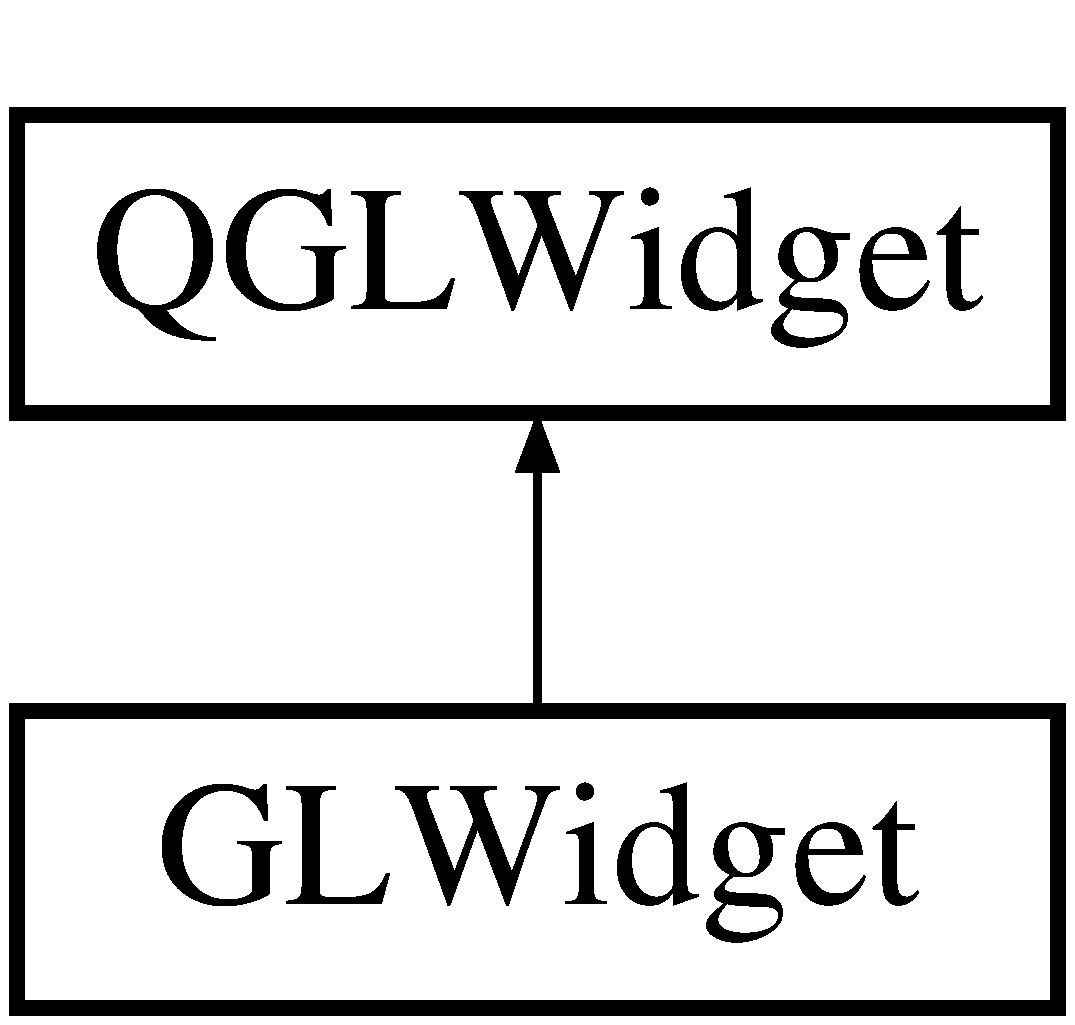
\includegraphics[height=2.000000cm]{class_g_l_widget}
\end{center}
\end{figure}
\subsection*{Public Member Functions}
\begin{DoxyCompactItemize}
\item 
\hypertarget{class_g_l_widget_ab79c391c86de1ffb76f6950b49d82c0c}{{\bfseries G\+L\+Widget} (Q\+Widget $\ast$parent=0)}\label{class_g_l_widget_ab79c391c86de1ffb76f6950b49d82c0c}

\item 
void \hyperlink{class_g_l_widget_ac0d2a8ecf60907a81c0d73475d851025}{resize\+G\+L} (int width, int height)
\begin{DoxyCompactList}\small\item\em Occurs when widget is resized. \end{DoxyCompactList}\item 
Q\+Size \hyperlink{class_g_l_widget_a57698bc426052845b43a135a13540154}{size\+Hint} () const 
\begin{DoxyCompactList}\small\item\em Set size of window. \end{DoxyCompactList}\item 
Q\+Size \hyperlink{class_g_l_widget_ade3142625c1bfda0576e419b176cf8b1}{minimum\+Size\+Hint} () const 
\begin{DoxyCompactList}\small\item\em Minimum size of window. \end{DoxyCompactList}\item 
\hypertarget{class_g_l_widget_a3947bf1a616e02627b92efb202ffc678}{void {\bfseries add\+Face} (const \hyperlink{class_mesh}{Mesh} $\ast$f)}\label{class_g_l_widget_a3947bf1a616e02627b92efb202ffc678}

\item 
\hypertarget{class_g_l_widget_a80be0cd34782a9d2d34b4c50f8605f6e}{void {\bfseries add\+Landmarks} (\hyperlink{class_landmarks}{Landmarks} $\ast$landmarks)}\label{class_g_l_widget_a80be0cd34782a9d2d34b4c50f8605f6e}

\item 
\hypertarget{class_g_l_widget_a517e3a0f84e2bacd25e0f861c8ecc5d4}{void {\bfseries add\+Curve} (Q\+Vector$<$ cv\+::\+Point3d $>$ \&curve)}\label{class_g_l_widget_a517e3a0f84e2bacd25e0f861c8ecc5d4}

\item 
\hypertarget{class_g_l_widget_ac1f9329242410b4e5fd256a6d84f9aa7}{void \hyperlink{class_g_l_widget_ac1f9329242410b4e5fd256a6d84f9aa7}{delete\+All} ()}\label{class_g_l_widget_ac1f9329242410b4e5fd256a6d84f9aa7}

\begin{DoxyCompactList}\small\item\em Delete all painted object. \end{DoxyCompactList}\item 
\hypertarget{class_g_l_widget_a2c2339ade3be153ffa90223e568dd470}{void \hyperlink{class_g_l_widget_a2c2339ade3be153ffa90223e568dd470}{clear\+All} ()}\label{class_g_l_widget_a2c2339ade3be153ffa90223e568dd470}

\begin{DoxyCompactList}\small\item\em Clear all painted object. \end{DoxyCompactList}\item 
\hypertarget{class_g_l_widget_aad214e6cbfd0d5f38a9a26aa9d1177b8}{const \hyperlink{class_mesh}{Mesh} $\ast$ {\bfseries get\+Face} ()}\label{class_g_l_widget_aad214e6cbfd0d5f38a9a26aa9d1177b8}

\end{DoxyCompactItemize}
\subsection*{Protected Member Functions}
\begin{DoxyCompactItemize}
\item 
\hypertarget{class_g_l_widget_ac25c4189967c4f728dc94fb96e22fc65}{void \hyperlink{class_g_l_widget_ac25c4189967c4f728dc94fb96e22fc65}{init} ()}\label{class_g_l_widget_ac25c4189967c4f728dc94fb96e22fc65}

\begin{DoxyCompactList}\small\item\em Initialization. \end{DoxyCompactList}\item 
\hypertarget{class_g_l_widget_a7fab13e8cc9fc0730ca54c08b2c923a7}{void \hyperlink{class_g_l_widget_a7fab13e8cc9fc0730ca54c08b2c923a7}{initialize\+G\+L} ()}\label{class_g_l_widget_a7fab13e8cc9fc0730ca54c08b2c923a7}

\begin{DoxyCompactList}\small\item\em Initializa Open\+G\+L. \end{DoxyCompactList}\item 
\hypertarget{class_g_l_widget_a640b5570cb2b37724fd5b58a77339c5e}{void \hyperlink{class_g_l_widget_a640b5570cb2b37724fd5b58a77339c5e}{paint\+G\+L} ()}\label{class_g_l_widget_a640b5570cb2b37724fd5b58a77339c5e}

\begin{DoxyCompactList}\small\item\em Paint faces. \end{DoxyCompactList}\item 
\hypertarget{class_g_l_widget_ab144cc8064c1bbf6d0ef0646ca0bd06c}{void {\bfseries mouse\+Press\+Event} (Q\+Mouse\+Event $\ast$event)}\label{class_g_l_widget_ab144cc8064c1bbf6d0ef0646ca0bd06c}

\item 
\hypertarget{class_g_l_widget_a9043bac13d6f0a5307ea5c7f9b3caa50}{void {\bfseries mouse\+Move\+Event} (Q\+Mouse\+Event $\ast$event)}\label{class_g_l_widget_a9043bac13d6f0a5307ea5c7f9b3caa50}

\item 
\hypertarget{class_g_l_widget_ab992c4c25439a5ef23031991015451c1}{void {\bfseries mouse\+Release\+Event} (Q\+Mouse\+Event $\ast$event)}\label{class_g_l_widget_ab992c4c25439a5ef23031991015451c1}

\end{DoxyCompactItemize}


\subsection{Detailed Description}
Class for painting mesh. 

\subsection{Member Function Documentation}
\hypertarget{class_g_l_widget_ade3142625c1bfda0576e419b176cf8b1}{\index{G\+L\+Widget@{G\+L\+Widget}!minimum\+Size\+Hint@{minimum\+Size\+Hint}}
\index{minimum\+Size\+Hint@{minimum\+Size\+Hint}!G\+L\+Widget@{G\+L\+Widget}}
\subsubsection[{minimum\+Size\+Hint}]{\setlength{\rightskip}{0pt plus 5cm}Q\+Size G\+L\+Widget\+::minimum\+Size\+Hint (
\begin{DoxyParamCaption}
{}
\end{DoxyParamCaption}
) const}}\label{class_g_l_widget_ade3142625c1bfda0576e419b176cf8b1}


Minimum size of window. 

\begin{DoxyReturn}{Returns}
Size of window 
\end{DoxyReturn}
\hypertarget{class_g_l_widget_ac0d2a8ecf60907a81c0d73475d851025}{\index{G\+L\+Widget@{G\+L\+Widget}!resize\+G\+L@{resize\+G\+L}}
\index{resize\+G\+L@{resize\+G\+L}!G\+L\+Widget@{G\+L\+Widget}}
\subsubsection[{resize\+G\+L}]{\setlength{\rightskip}{0pt plus 5cm}void G\+L\+Widget\+::resize\+G\+L (
\begin{DoxyParamCaption}
\item[{int}]{width, }
\item[{int}]{height}
\end{DoxyParamCaption}
)}}\label{class_g_l_widget_ac0d2a8ecf60907a81c0d73475d851025}


Occurs when widget is resized. 


\begin{DoxyParams}{Parameters}
{\em width} & New width \\
\hline
{\em height} & New height \\
\hline
\end{DoxyParams}
\hypertarget{class_g_l_widget_a57698bc426052845b43a135a13540154}{\index{G\+L\+Widget@{G\+L\+Widget}!size\+Hint@{size\+Hint}}
\index{size\+Hint@{size\+Hint}!G\+L\+Widget@{G\+L\+Widget}}
\subsubsection[{size\+Hint}]{\setlength{\rightskip}{0pt plus 5cm}Q\+Size G\+L\+Widget\+::size\+Hint (
\begin{DoxyParamCaption}
{}
\end{DoxyParamCaption}
) const}}\label{class_g_l_widget_a57698bc426052845b43a135a13540154}


Set size of window. 

\begin{DoxyReturn}{Returns}
Window size 
\end{DoxyReturn}


The documentation for this class was generated from the following files\+:\begin{DoxyCompactItemize}
\item 
glwidget.\+h\item 
glwidget.\+cpp\end{DoxyCompactItemize}

\hypertarget{class_landmark_detector}{\section{Landmark\+Detector Class Reference}
\label{class_landmark_detector}\index{Landmark\+Detector@{Landmark\+Detector}}
}


Class for landmark detection.  




{\ttfamily \#include $<$landmarkdetector.\+h$>$}

\subsection*{Public Member Functions}
\begin{DoxyCompactItemize}
\item 
\hypertarget{class_landmark_detector_ab1b5f48ca28480126aa72016e5f27456}{{\bfseries Landmark\+Detector} (cv\+::\+Mat depth\+Map)}\label{class_landmark_detector_ab1b5f48ca28480126aa72016e5f27456}

\item 
\hypertarget{class_landmark_detector_ab7d2787e5bff6190b282710f40a81467}{void \hyperlink{class_landmark_detector_ab7d2787e5bff6190b282710f40a81467}{detect\+Nose\+Tip} ()}\label{class_landmark_detector_ab7d2787e5bff6190b282710f40a81467}

\begin{DoxyCompactList}\small\item\em Detect nose tip. \end{DoxyCompactList}\item 
\hypertarget{class_landmark_detector_a197a7813b3f023433fb19c1928e173b0}{void \hyperlink{class_landmark_detector_a197a7813b3f023433fb19c1928e173b0}{detect\+Nose\+Root} ()}\label{class_landmark_detector_a197a7813b3f023433fb19c1928e173b0}

\begin{DoxyCompactList}\small\item\em Detect nose root. \end{DoxyCompactList}\item 
\hypertarget{class_landmark_detector_a842700d6ba9db23adf9f9308a45eb30d}{void \hyperlink{class_landmark_detector_a842700d6ba9db23adf9f9308a45eb30d}{detect\+Nose\+Corners} ()}\label{class_landmark_detector_a842700d6ba9db23adf9f9308a45eb30d}

\begin{DoxyCompactList}\small\item\em Detect nose corners. \end{DoxyCompactList}\item 
\hypertarget{class_landmark_detector_a5b4a55e448e6e6f5d0885a2f9d87bf2d}{void \hyperlink{class_landmark_detector_a5b4a55e448e6e6f5d0885a2f9d87bf2d}{detect\+Inner\+Eye\+Corners} ()}\label{class_landmark_detector_a5b4a55e448e6e6f5d0885a2f9d87bf2d}

\begin{DoxyCompactList}\small\item\em Detect inner eye corners. \end{DoxyCompactList}\item 
\hypertarget{class_landmark_detector_aa3c53cac45cfc7605b0f7ad85a5e8ca7}{void \hyperlink{class_landmark_detector_aa3c53cac45cfc7605b0f7ad85a5e8ca7}{detect\+Nose\+Bottom} ()}\label{class_landmark_detector_aa3c53cac45cfc7605b0f7ad85a5e8ca7}

\begin{DoxyCompactList}\small\item\em Detect nose bottom. \end{DoxyCompactList}\item 
bool \hyperlink{class_landmark_detector_a05ccf70a8911910dcdea9b07dc5dc0bc}{detect\+All} (\hyperlink{class_landmarks}{Landmarks} \&landmarks)
\begin{DoxyCompactList}\small\item\em Detect all landmarks. \end{DoxyCompactList}\end{DoxyCompactItemize}
\subsection*{Static Public Member Functions}
\begin{DoxyCompactItemize}
\item 
static bool \hyperlink{class_landmark_detector_aa2c1f6f7e3761542be61143bc71c2927}{check\+Landmarks} (\hyperlink{class_landmarks}{Landmarks} \&src\+Landmarks, \hyperlink{class_landmarks}{Landmarks} \&ref\+Landmarks)
\begin{DoxyCompactList}\small\item\em Check distance between two landmarks sets. \end{DoxyCompactList}\end{DoxyCompactItemize}
\subsection*{Public Attributes}
\begin{DoxyCompactItemize}
\item 
\hypertarget{class_landmark_detector_a11f027af8a1ae3515d8371b7df1c2e88}{cv\+::\+Point {\bfseries nose\+Tip}}\label{class_landmark_detector_a11f027af8a1ae3515d8371b7df1c2e88}

\item 
\hypertarget{class_landmark_detector_a9cd890a65aad92f3a90aa2ea0c051a73}{cv\+::\+Point {\bfseries nose\+Root}}\label{class_landmark_detector_a9cd890a65aad92f3a90aa2ea0c051a73}

\item 
\hypertarget{class_landmark_detector_a63dea171e498afd5b1ea3d5561ec63bb}{cv\+::\+Point {\bfseries eye\+Inner\+Corner\+Left}}\label{class_landmark_detector_a63dea171e498afd5b1ea3d5561ec63bb}

\item 
\hypertarget{class_landmark_detector_ad8ddb3fce40489e398bc1dd055d3e936}{cv\+::\+Point {\bfseries eye\+Inner\+Corner\+Right}}\label{class_landmark_detector_ad8ddb3fce40489e398bc1dd055d3e936}

\item 
\hypertarget{class_landmark_detector_aabda0f65b4d054befd2115408c33420d}{cv\+::\+Point {\bfseries nose\+Corner\+Left}}\label{class_landmark_detector_aabda0f65b4d054befd2115408c33420d}

\item 
\hypertarget{class_landmark_detector_aba55847250b8ec56c64e085d90b42615}{cv\+::\+Point {\bfseries nose\+Corner\+Right}}\label{class_landmark_detector_aba55847250b8ec56c64e085d90b42615}

\item 
\hypertarget{class_landmark_detector_a523f207dd4d020c2a157c907a2172ec9}{cv\+::\+Point {\bfseries nose\+Bottom}}\label{class_landmark_detector_a523f207dd4d020c2a157c907a2172ec9}

\end{DoxyCompactItemize}


\subsection{Detailed Description}
Class for landmark detection. 

\subsection{Member Function Documentation}
\hypertarget{class_landmark_detector_aa2c1f6f7e3761542be61143bc71c2927}{\index{Landmark\+Detector@{Landmark\+Detector}!check\+Landmarks@{check\+Landmarks}}
\index{check\+Landmarks@{check\+Landmarks}!Landmark\+Detector@{Landmark\+Detector}}
\subsubsection[{check\+Landmarks}]{\setlength{\rightskip}{0pt plus 5cm}bool Landmark\+Detector\+::check\+Landmarks (
\begin{DoxyParamCaption}
\item[{{\bf Landmarks} \&}]{src\+Landmarks, }
\item[{{\bf Landmarks} \&}]{ref\+Landmarks}
\end{DoxyParamCaption}
)\hspace{0.3cm}{\ttfamily [static]}}}\label{class_landmark_detector_aa2c1f6f7e3761542be61143bc71c2927}


Check distance between two landmarks sets. 


\begin{DoxyParams}{Parameters}
{\em src\+Landmarks} & Source landmark \\
\hline
{\em ref\+Landmarks} & Reference landmark \\
\hline
\end{DoxyParams}
\begin{DoxyReturn}{Returns}
True if distance is ok. 
\end{DoxyReturn}
\hypertarget{class_landmark_detector_a05ccf70a8911910dcdea9b07dc5dc0bc}{\index{Landmark\+Detector@{Landmark\+Detector}!detect\+All@{detect\+All}}
\index{detect\+All@{detect\+All}!Landmark\+Detector@{Landmark\+Detector}}
\subsubsection[{detect\+All}]{\setlength{\rightskip}{0pt plus 5cm}bool Landmark\+Detector\+::detect\+All (
\begin{DoxyParamCaption}
\item[{{\bf Landmarks} \&}]{landmarks}
\end{DoxyParamCaption}
)}}\label{class_landmark_detector_a05ccf70a8911910dcdea9b07dc5dc0bc}


Detect all landmarks. 


\begin{DoxyParams}{Parameters}
{\em Vector} & of landmarks to store it. \\
\hline
\end{DoxyParams}
\begin{DoxyReturn}{Returns}
True if no exeption during detection appears 
\end{DoxyReturn}


The documentation for this class was generated from the following files\+:\begin{DoxyCompactItemize}
\item 
landmarkdetector.\+h\item 
landmarkdetector.\+cpp\end{DoxyCompactItemize}

\hypertarget{class_landmarks}{\section{Landmarks Class Reference}
\label{class_landmarks}\index{Landmarks@{Landmarks}}
}


Class for store landmarks position.  




{\ttfamily \#include $<$landmarks.\+h$>$}

\subsection*{Public Types}
\begin{DoxyCompactItemize}
\item 
\hypertarget{class_landmarks_a69362bef3ef2209cb2304ff7ea2ce91e}{enum \hyperlink{class_landmarks_a69362bef3ef2209cb2304ff7ea2ce91e}{Landmark\+Names} \{ \\*
{\bfseries Nose\+Tip} = 0, 
{\bfseries Nose\+Corner\+Left} = 1, 
{\bfseries Nose\+Corner\+Right} = 2, 
{\bfseries Nose\+Bottom} = 3, 
\\*
{\bfseries Nose\+Root} = 4, 
{\bfseries Eye\+Inner\+Corner\+Left} = 5, 
{\bfseries Eye\+Inner\+Corner\+Right} = 6
 \}}\label{class_landmarks_a69362bef3ef2209cb2304ff7ea2ce91e}

\begin{DoxyCompactList}\small\item\em Types of landmark. \end{DoxyCompactList}\end{DoxyCompactItemize}
\subsection*{Public Member Functions}
\begin{DoxyCompactItemize}
\item 
\hyperlink{class_landmarks_ad97ffa895a71e45b208ab4eb2fbd96ae}{Landmarks} (Vector\+Of\+Landmarks \+\_\+landmarks)
\begin{DoxyCompactList}\small\item\em Constructor. Initialize by vector of landmarks. \end{DoxyCompactList}\item 
\hyperlink{class_landmarks_a2d070b7086463daaa617c946c4576ae8}{Landmarks} (Q\+String file\+Name, Q\+String load\+Path=Common\+::path\+To\+Landmark\+Dir)
\begin{DoxyCompactList}\small\item\em Constructor. Initialized by values from file. \end{DoxyCompactList}\item 
cv\+::\+Point \hyperlink{class_landmarks_a24e9344ab527627e7aa9077ed1f39509}{pos} (\hyperlink{class_landmarks_a69362bef3ef2209cb2304ff7ea2ce91e}{Landmarks\+::\+Landmark\+Names} name)
\begin{DoxyCompactList}\small\item\em Get position of landmark. \end{DoxyCompactList}\item 
bool \hyperlink{class_landmarks_ad3d8c6a24f384016eaba29d078921350}{is} (\hyperlink{class_landmarks_a69362bef3ef2209cb2304ff7ea2ce91e}{Landmarks\+::\+Landmark\+Names} name)
\begin{DoxyCompactList}\small\item\em Check if landmarh has been set. \end{DoxyCompactList}\item 
void \hyperlink{class_landmarks_af52da543b2d0ece5bb17dbf7cbe6b6e9}{set} (\hyperlink{class_landmarks_a69362bef3ef2209cb2304ff7ea2ce91e}{Landmarks\+::\+Landmark\+Names} name, cv\+::\+Point \hyperlink{class_landmarks_a24e9344ab527627e7aa9077ed1f39509}{pos})
\begin{DoxyCompactList}\small\item\em Set position of landmark. \end{DoxyCompactList}\item 
void \hyperlink{class_landmarks_ae64ebc983fa10e85ab63768936c1a0ba}{discard} (\hyperlink{class_landmarks_a69362bef3ef2209cb2304ff7ea2ce91e}{Landmarks\+::\+Landmark\+Names} name)
\begin{DoxyCompactList}\small\item\em Unset landmark position. \end{DoxyCompactList}\item 
void \hyperlink{class_landmarks_a7a83b5a94c23acefe755ca2d9cad7a7d}{save} (Q\+String file\+Name, Q\+String save\+Path=Common\+::path\+To\+Landmark\+Dir)
\begin{DoxyCompactList}\small\item\em Save landmarks to file. \end{DoxyCompactList}\item 
void \hyperlink{class_landmarks_ac0d7586eae8bcc28ce1783667df6a415}{load} (Q\+String file\+Name, Q\+String load\+Path=Common\+::path\+To\+Landmark\+Dir)
\begin{DoxyCompactList}\small\item\em Load landmarks to file. \end{DoxyCompactList}\item 
Vector\+Of\+Landmarks \hyperlink{class_landmarks_a2b30a752fa58794414e338b3fc7a2fe9}{get\+Landmarks} ()
\begin{DoxyCompactList}\small\item\em Get vector of landmarks. \end{DoxyCompactList}\item 
void \hyperlink{class_landmarks_ac6c4346445e2441a212d839de99ecdca}{scale} (float scale\+Factor)
\begin{DoxyCompactList}\small\item\em Multiple landmarks position by value. \end{DoxyCompactList}\end{DoxyCompactItemize}


\subsection{Detailed Description}
Class for store landmarks position. 

\subsection{Constructor \& Destructor Documentation}
\hypertarget{class_landmarks_ad97ffa895a71e45b208ab4eb2fbd96ae}{\index{Landmarks@{Landmarks}!Landmarks@{Landmarks}}
\index{Landmarks@{Landmarks}!Landmarks@{Landmarks}}
\subsubsection[{Landmarks}]{\setlength{\rightskip}{0pt plus 5cm}Landmarks\+::\+Landmarks (
\begin{DoxyParamCaption}
\item[{Vector\+Of\+Landmarks}]{landmarks}
\end{DoxyParamCaption}
)}}\label{class_landmarks_ad97ffa895a71e45b208ab4eb2fbd96ae}


Constructor. Initialize by vector of landmarks. 


\begin{DoxyParams}{Parameters}
{\em landmarks} & Vector of landmarks \\
\hline
\end{DoxyParams}
\hypertarget{class_landmarks_a2d070b7086463daaa617c946c4576ae8}{\index{Landmarks@{Landmarks}!Landmarks@{Landmarks}}
\index{Landmarks@{Landmarks}!Landmarks@{Landmarks}}
\subsubsection[{Landmarks}]{\setlength{\rightskip}{0pt plus 5cm}Landmarks\+::\+Landmarks (
\begin{DoxyParamCaption}
\item[{Q\+String}]{file\+Name, }
\item[{Q\+String}]{load\+Path = {\ttfamily Common\+:\+:pathToLandmarkDir}}
\end{DoxyParamCaption}
)}}\label{class_landmarks_a2d070b7086463daaa617c946c4576ae8}


Constructor. Initialized by values from file. 


\begin{DoxyParams}{Parameters}
{\em file\+Name} & File with Vector of landmarks. \\
\hline
{\em load\+Path} & Directory with file. \\
\hline
\end{DoxyParams}


\subsection{Member Function Documentation}
\hypertarget{class_landmarks_ae64ebc983fa10e85ab63768936c1a0ba}{\index{Landmarks@{Landmarks}!discard@{discard}}
\index{discard@{discard}!Landmarks@{Landmarks}}
\subsubsection[{discard}]{\setlength{\rightskip}{0pt plus 5cm}void Landmarks\+::discard (
\begin{DoxyParamCaption}
\item[{{\bf Landmarks\+::\+Landmark\+Names}}]{name}
\end{DoxyParamCaption}
)}}\label{class_landmarks_ae64ebc983fa10e85ab63768936c1a0ba}


Unset landmark position. 


\begin{DoxyParams}{Parameters}
{\em name} & Landmark name \\
\hline
\end{DoxyParams}
\hypertarget{class_landmarks_a2b30a752fa58794414e338b3fc7a2fe9}{\index{Landmarks@{Landmarks}!get\+Landmarks@{get\+Landmarks}}
\index{get\+Landmarks@{get\+Landmarks}!Landmarks@{Landmarks}}
\subsubsection[{get\+Landmarks}]{\setlength{\rightskip}{0pt plus 5cm}Vector\+Of\+Landmarks Landmarks\+::get\+Landmarks (
\begin{DoxyParamCaption}
{}
\end{DoxyParamCaption}
)}}\label{class_landmarks_a2b30a752fa58794414e338b3fc7a2fe9}


Get vector of landmarks. 

\begin{DoxyReturn}{Returns}
Vector of landmarks 
\end{DoxyReturn}
\hypertarget{class_landmarks_ad3d8c6a24f384016eaba29d078921350}{\index{Landmarks@{Landmarks}!is@{is}}
\index{is@{is}!Landmarks@{Landmarks}}
\subsubsection[{is}]{\setlength{\rightskip}{0pt plus 5cm}bool Landmarks\+::is (
\begin{DoxyParamCaption}
\item[{{\bf Landmarks\+::\+Landmark\+Names}}]{name}
\end{DoxyParamCaption}
)}}\label{class_landmarks_ad3d8c6a24f384016eaba29d078921350}


Check if landmarh has been set. 


\begin{DoxyParams}{Parameters}
{\em name} & Landmark name \\
\hline
\end{DoxyParams}
\begin{DoxyReturn}{Returns}
Dicision 
\end{DoxyReturn}
\hypertarget{class_landmarks_ac0d7586eae8bcc28ce1783667df6a415}{\index{Landmarks@{Landmarks}!load@{load}}
\index{load@{load}!Landmarks@{Landmarks}}
\subsubsection[{load}]{\setlength{\rightskip}{0pt plus 5cm}void Landmarks\+::load (
\begin{DoxyParamCaption}
\item[{Q\+String}]{file\+Name, }
\item[{Q\+String}]{load\+Path = {\ttfamily Common\+:\+:pathToLandmarkDir}}
\end{DoxyParamCaption}
)}}\label{class_landmarks_ac0d7586eae8bcc28ce1783667df6a415}


Load landmarks to file. 


\begin{DoxyParams}{Parameters}
{\em file\+Name} & File to load \\
\hline
{\em load\+Path} & Directory with file \\
\hline
\end{DoxyParams}
\hypertarget{class_landmarks_a24e9344ab527627e7aa9077ed1f39509}{\index{Landmarks@{Landmarks}!pos@{pos}}
\index{pos@{pos}!Landmarks@{Landmarks}}
\subsubsection[{pos}]{\setlength{\rightskip}{0pt plus 5cm}cv\+::\+Point Landmarks\+::pos (
\begin{DoxyParamCaption}
\item[{{\bf Landmarks\+::\+Landmark\+Names}}]{name}
\end{DoxyParamCaption}
)}}\label{class_landmarks_a24e9344ab527627e7aa9077ed1f39509}


Get position of landmark. 


\begin{DoxyParams}{Parameters}
{\em name} & Landmark name \\
\hline
\end{DoxyParams}
\begin{DoxyReturn}{Returns}
Position 
\end{DoxyReturn}
\hypertarget{class_landmarks_a7a83b5a94c23acefe755ca2d9cad7a7d}{\index{Landmarks@{Landmarks}!save@{save}}
\index{save@{save}!Landmarks@{Landmarks}}
\subsubsection[{save}]{\setlength{\rightskip}{0pt plus 5cm}void Landmarks\+::save (
\begin{DoxyParamCaption}
\item[{Q\+String}]{file\+Name, }
\item[{Q\+String}]{save\+Path = {\ttfamily Common\+:\+:pathToLandmarkDir}}
\end{DoxyParamCaption}
)}}\label{class_landmarks_a7a83b5a94c23acefe755ca2d9cad7a7d}


Save landmarks to file. 


\begin{DoxyParams}{Parameters}
{\em file\+Name} & File to save \\
\hline
{\em save\+Path} & Directory with file \\
\hline
\end{DoxyParams}
\hypertarget{class_landmarks_ac6c4346445e2441a212d839de99ecdca}{\index{Landmarks@{Landmarks}!scale@{scale}}
\index{scale@{scale}!Landmarks@{Landmarks}}
\subsubsection[{scale}]{\setlength{\rightskip}{0pt plus 5cm}void Landmarks\+::scale (
\begin{DoxyParamCaption}
\item[{float}]{scale\+Factor}
\end{DoxyParamCaption}
)}}\label{class_landmarks_ac6c4346445e2441a212d839de99ecdca}


Multiple landmarks position by value. 


\begin{DoxyParams}{Parameters}
{\em scale\+Factor} & Value to mulitple \\
\hline
\end{DoxyParams}
\hypertarget{class_landmarks_af52da543b2d0ece5bb17dbf7cbe6b6e9}{\index{Landmarks@{Landmarks}!set@{set}}
\index{set@{set}!Landmarks@{Landmarks}}
\subsubsection[{set}]{\setlength{\rightskip}{0pt plus 5cm}void Landmarks\+::set (
\begin{DoxyParamCaption}
\item[{{\bf Landmarks\+::\+Landmark\+Names}}]{name, }
\item[{cv\+::\+Point}]{pos}
\end{DoxyParamCaption}
)}}\label{class_landmarks_af52da543b2d0ece5bb17dbf7cbe6b6e9}


Set position of landmark. 


\begin{DoxyParams}{Parameters}
{\em name} & Landmark name \\
\hline
{\em pos} & Landmark position \\
\hline
\end{DoxyParams}


The documentation for this class was generated from the following files\+:\begin{DoxyCompactItemize}
\item 
landmarks.\+h\item 
landmarks.\+cpp\end{DoxyCompactItemize}

\hypertarget{class_main_window}{\section{Main\+Window Class Reference}
\label{class_main_window}\index{Main\+Window@{Main\+Window}}
}


Need for show up models of face.  




{\ttfamily \#include $<$mainwindow.\+h$>$}

Inheritance diagram for Main\+Window\+:\begin{figure}[H]
\begin{center}
\leavevmode
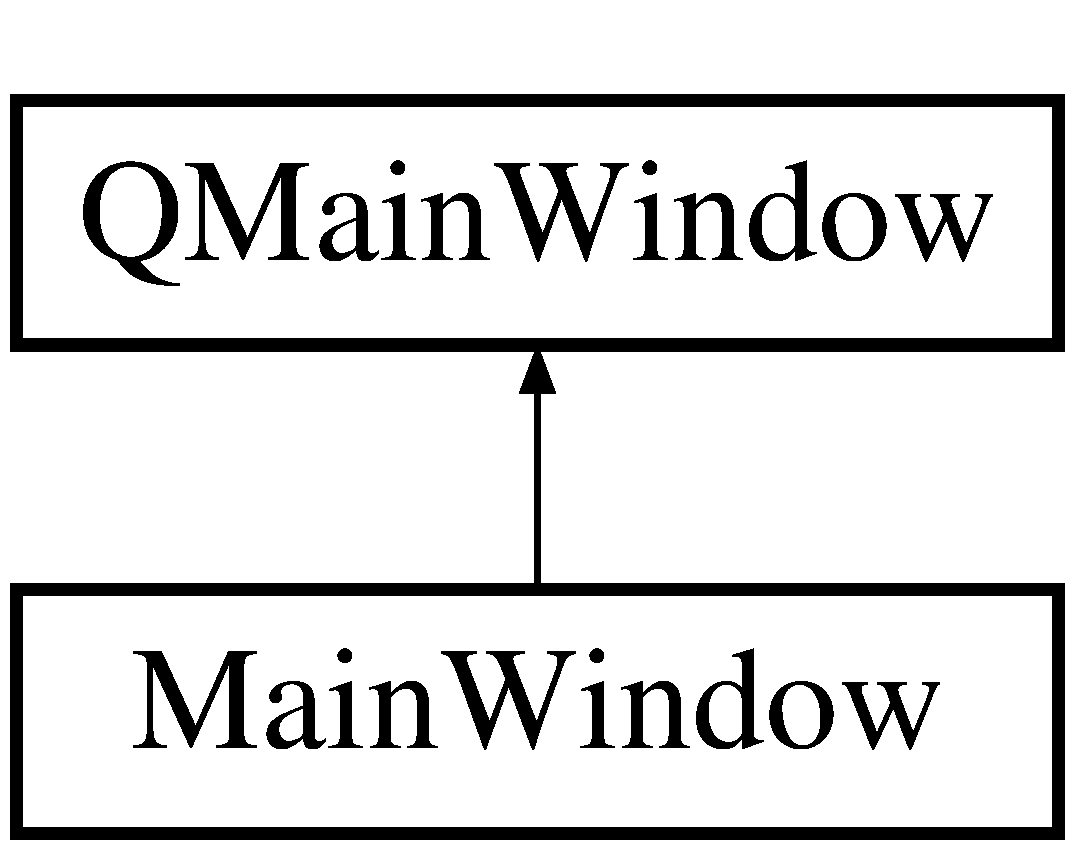
\includegraphics[height=2.000000cm]{class_main_window}
\end{center}
\end{figure}
\subsection*{Public Member Functions}
\begin{DoxyCompactItemize}
\item 
\hypertarget{class_main_window_a8b244be8b7b7db1b08de2a2acb9409db}{{\bfseries Main\+Window} (Q\+Widget $\ast$parent=0)}\label{class_main_window_a8b244be8b7b7db1b08de2a2acb9409db}

\end{DoxyCompactItemize}


\subsection{Detailed Description}
Need for show up models of face. 

The documentation for this class was generated from the following files\+:\begin{DoxyCompactItemize}
\item 
mainwindow.\+h\item 
mainwindow.\+cpp\end{DoxyCompactItemize}

\hypertarget{class_mesh}{\section{Mesh Class Reference}
\label{class_mesh}\index{Mesh@{Mesh}}
}


Class for represent 3\+D model of face.  




{\ttfamily \#include $<$mesh.\+h$>$}

\subsection*{Public Types}
\begin{DoxyCompactItemize}
\item 
\hypertarget{class_mesh_a6fbf5a0481dcee54f0ea44363c7de2b7}{typedef cv\+::\+Vec3i {\bfseries Triangle}}\label{class_mesh_a6fbf5a0481dcee54f0ea44363c7de2b7}

\item 
\hypertarget{class_mesh_a4449aba0563ba3e8985ae1a96dbb7f06}{typedef cv\+::\+Vec3b {\bfseries Color}}\label{class_mesh_a4449aba0563ba3e8985ae1a96dbb7f06}

\item 
\hypertarget{class_mesh_ac5052738062f59eef6517606d748f804}{typedef Q\+Vector$<$ Triangle $>$ {\bfseries Triangles}}\label{class_mesh_ac5052738062f59eef6517606d748f804}

\item 
\hypertarget{class_mesh_a41a96d934a45bf52f091f33c099fbd0d}{typedef Q\+Vector$<$ Color $>$ {\bfseries Colors}}\label{class_mesh_a41a96d934a45bf52f091f33c099fbd0d}

\end{DoxyCompactItemize}
\subsection*{Public Member Functions}
\begin{DoxyCompactItemize}
\item 
\hypertarget{class_mesh_a2af137f1571af89172b9c102302c416b}{\hyperlink{class_mesh_a2af137f1571af89172b9c102302c416b}{Mesh} ()}\label{class_mesh_a2af137f1571af89172b9c102302c416b}

\begin{DoxyCompactList}\small\item\em Constructor. \end{DoxyCompactList}\item 
\hyperlink{class_mesh_a364ba4b2fd09e26795e68f9aa9c46d7d}{Mesh} (const \hyperlink{class_mesh}{Mesh} \&src)
\begin{DoxyCompactList}\small\item\em Constructor. \end{DoxyCompactList}\item 
\hyperlink{class_mesh_a4b17a8a6b16ef6751e30d7efab345ebf}{Mesh} (const Q\+String path, bool centralize\+Loaded\+Mesh=false)
\begin{DoxyCompactList}\small\item\em Constructor. Create mesh from 3d model stored in file. \end{DoxyCompactList}\item 
\hypertarget{class_mesh_a38a2694f262d993b4b50f53e20599031}{void \hyperlink{class_mesh_a38a2694f262d993b4b50f53e20599031}{print\+Stats} ()}\label{class_mesh_a38a2694f262d993b4b50f53e20599031}

\begin{DoxyCompactList}\small\item\em Print stats of mesh. \end{DoxyCompactList}\item 
\hypertarget{class_mesh_aa34d69f670ed6e1ebc101062dee17ad4}{void \hyperlink{class_mesh_aa34d69f670ed6e1ebc101062dee17ad4}{centralize} ()}\label{class_mesh_aa34d69f670ed6e1ebc101062dee17ad4}

\begin{DoxyCompactList}\small\item\em Translate centroid of mesh to point (0,0,0) \end{DoxyCompactList}\item 
void \hyperlink{class_mesh_aae3c2893ee25abbff8feea44d724ddb4}{translate} (cv\+::\+Point3d translation\+Vector)
\begin{DoxyCompactList}\small\item\em Translate mesh. \end{DoxyCompactList}\item 
void \hyperlink{class_mesh_a8f1702ee51f0c3d0bd980c665b5d6952}{transform} (Matrix \&m)
\begin{DoxyCompactList}\small\item\em Transform mesh. \end{DoxyCompactList}\item 
void \hyperlink{class_mesh_a89e4e340939aa89534978c60ca690466}{rotate} (double x, double y, double z)
\begin{DoxyCompactList}\small\item\em Rotate mesh. \end{DoxyCompactList}\item 
\hyperlink{class_mesh}{Mesh} \hyperlink{class_mesh_a0b6bce98a99444eb3daf42d213ba89ab}{crop} (cv\+::\+Point3d center, int delta\+P\+X, int delta\+M\+X, int delta\+P\+Y, int delta\+M\+Y)
\begin{DoxyCompactList}\small\item\em Crop mesh by distances from center point. \end{DoxyCompactList}\item 
\hyperlink{class_mesh}{Mesh} \hyperlink{class_mesh_a1ebf5c007fa538e183d06cb021c6fac4}{crop} (cv\+::\+Point3d top\+Left, cv\+::\+Point3d bottom\+Right)
\begin{DoxyCompactList}\small\item\em Crop mesh by points. \end{DoxyCompactList}\item 
void \hyperlink{class_mesh_ab7eda900a4a92c5eee9eeb7a6c65d09a}{crop\+Me} (cv\+::\+Point2d top\+Left, cv\+::\+Point2d bottom\+Right)
\begin{DoxyCompactList}\small\item\em Crop mesh by points. \end{DoxyCompactList}\item 
\hyperlink{class_mesh}{Mesh} \hyperlink{class_mesh_a10b3d6d6b111a68eb380e7e125a8bfd2}{z\+Level\+Select} (double z\+Value)
\begin{DoxyCompactList}\small\item\em Extract mesh by asix Z. \end{DoxyCompactList}\item 
\hyperlink{class_mesh}{Mesh} \hyperlink{class_mesh_a549432bc9872781b714f3740dd976086}{radius\+Select} (double radius, cv\+::\+Point3d center=cv\+::\+Point3d(0, 0, 0))
\begin{DoxyCompactList}\small\item\em Extract mesh by radius. \end{DoxyCompactList}\item 
void \hyperlink{class_mesh_a822182ddb8a31b9e7c10727a10404ad3}{write\+O\+B\+J} (const Q\+String \&path, char decimal\+Point)
\begin{DoxyCompactList}\small\item\em Save mesh as O\+B\+J 3d model. \end{DoxyCompactList}\item 
void \hyperlink{class_mesh_a017e0441fdff322922dc1090b04d3c37}{load\+From\+A\+B\+S} (const Q\+String \&filename, bool centralize\+Loaded\+Mesh=false)
\begin{DoxyCompactList}\small\item\em Create mesh from A\+B\+S 3d model. \end{DoxyCompactList}\item 
void \hyperlink{class_mesh_a803901209c07edc0b7c3904eccac40bc}{load\+From\+O\+B\+J} (const Q\+String \&filename, bool centralize\+Loaded\+Mesh=false)
\begin{DoxyCompactList}\small\item\em Create depthmap from O\+B\+J 3d model. \end{DoxyCompactList}\item 
void \hyperlink{class_mesh_a87dc88824cf6604b494e774b54a7f0b1}{load\+From\+Pointcloud} (Vector\+Of\+Points \&pointcloud, bool centralize\+Loaded\+Mesh=false, bool \hyperlink{class_mesh_ad69edfbb7cde40edb166831358e0e5ac}{calculate\+Triangles}=true)
\begin{DoxyCompactList}\small\item\em Create mesh from point cloud. \end{DoxyCompactList}\item 
\hyperlink{class_mesh}{Mesh} \hyperlink{class_mesh_a2b8b2a62e220de4cc9e3e19c0a0a6071}{get\+Extract2d\+Grid} (\hyperlink{class_mesh}{Mesh} \&grid)
\begin{DoxyCompactList}\small\item\em Extract part of mesh. \end{DoxyCompactList}\item 
void \hyperlink{class_mesh_ad9fb7ec4fe3cd1f5a511654739029c33}{get\+Extract2d\+Grid} (\hyperlink{class_mesh}{Mesh} \&grid, \hyperlink{class_mesh}{Mesh} \&dst)
\begin{DoxyCompactList}\small\item\em \hyperlink{class_mesh_a2b8b2a62e220de4cc9e3e19c0a0a6071}{Mesh\+::get\+Extract2d\+Grid} -\/ extract grid from face, use only x,y coords. \end{DoxyCompactList}\item 
void \hyperlink{class_mesh_aa39be434d3573cd6b3e9de6d2f36502a}{get\+Extract2d\+Grid\+\_\+2} (\hyperlink{class_mesh}{Mesh} \&grid, \hyperlink{class_mesh}{Mesh} \&dst)
\begin{DoxyCompactList}\small\item\em \hyperlink{class_mesh_a2b8b2a62e220de4cc9e3e19c0a0a6071}{Mesh\+::get\+Extract2d\+Grid} Extract grid from face, used only x,y coords. if distance of closed point is higher then max\+Distance, skip it. \end{DoxyCompactList}\item 
\hyperlink{class_mesh}{Mesh} \hyperlink{class_mesh_a0752d96a941240e508b605281a3bb5f0}{get\+Closed\+Points} (\hyperlink{class_mesh}{Mesh} \&input\+Mesh, cv\+::flann\+::\+Index \&index, float $\ast$distance)
\begin{DoxyCompactList}\small\item\em Search nearest point for each point int mesh. \end{DoxyCompactList}\item 
\hypertarget{class_mesh_adb5c20ded833a9c01773acb2de4304d9}{float {\bfseries get\+Closed\+Distance} (cv\+::flann\+::\+Index \&index)}\label{class_mesh_adb5c20ded833a9c01773acb2de4304d9}

\item 
int \hyperlink{class_mesh_a2e91d8acdb1737e0eaf94576d8406a6e}{get\+Closed2d\+Point} (cv\+::\+Point2d point)
\begin{DoxyCompactList}\small\item\em Search closed point from mesh. \end{DoxyCompactList}\item 
cv\+::\+Point3d \hyperlink{class_mesh_a3a9fb77fbb9b1ff5b7a33ee5ab783b93}{get\+Mean\+Point} ()
\begin{DoxyCompactList}\small\item\em Compute mean point of mesh. \end{DoxyCompactList}\item 
Q\+Vector$<$ cv\+::\+Point3d $>$ $\ast$ \hyperlink{class_mesh_ae18bb93929f87c35f50122e7725e097e}{get\+Vector\+Of\+Point3d} ()
\begin{DoxyCompactList}\small\item\em Convert mesh to vector of point. \end{DoxyCompactList}\item 
\hypertarget{class_mesh_ad69edfbb7cde40edb166831358e0e5ac}{void \hyperlink{class_mesh_ad69edfbb7cde40edb166831358e0e5ac}{calculate\+Triangles} ()}\label{class_mesh_ad69edfbb7cde40edb166831358e0e5ac}

\begin{DoxyCompactList}\small\item\em Connect points to triangles. \end{DoxyCompactList}\item 
\hypertarget{class_mesh_a06ac6e1eb7bd66f5c85c0aab3e805500}{void \hyperlink{class_mesh_a06ac6e1eb7bd66f5c85c0aab3e805500}{recalculate\+Min\+Max} ()}\label{class_mesh_a06ac6e1eb7bd66f5c85c0aab3e805500}

\begin{DoxyCompactList}\small\item\em Recalculate minimum and maximum for each axis. \end{DoxyCompactList}\end{DoxyCompactItemize}
\subsection*{Static Public Member Functions}
\begin{DoxyCompactItemize}
\item 
static \hyperlink{class_mesh}{Mesh} \hyperlink{class_mesh_a76fdd1e644b1154f5b0d37e8631cef94}{from\+A\+B\+S} (const Q\+String \&filename, bool centralize\+Loaded\+Mesh=false)
\begin{DoxyCompactList}\small\item\em Create mesh from A\+B\+S 3d model. \end{DoxyCompactList}\item 
static \hyperlink{class_mesh}{Mesh} \hyperlink{class_mesh_aebd86dfd1696005226e3d7672942e54f}{from\+O\+B\+J} (const Q\+String \&filename, bool centralize\+Loaded\+Mesh=false)
\begin{DoxyCompactList}\small\item\em Create depthmap from O\+B\+J 3d model. \end{DoxyCompactList}\item 
static \hyperlink{class_mesh}{Mesh} \hyperlink{class_mesh_a406020ec939773954b3be638041573cc}{from\+Pointcloud} (Vector\+Of\+Points \&pointcloud, bool centralize\+Loaded\+Mesh=false, bool \hyperlink{class_mesh_ad69edfbb7cde40edb166831358e0e5ac}{calculate\+Triangles}=true)
\begin{DoxyCompactList}\small\item\em Create mesh from point cloud. \end{DoxyCompactList}\item 
static \hyperlink{class_mesh}{Mesh} \hyperlink{class_mesh_a07d0c4f5d683e4adda0e93c8578eb285}{create2d\+Grid} (cv\+::\+Point3d top\+Left, cv\+::\+Point3d bottom\+Right, int step\+X, int step\+Y)
\begin{DoxyCompactList}\small\item\em Creaete 3\+D grid. \end{DoxyCompactList}\item 
static void \hyperlink{class_mesh_a7644d8304dc1cac1e0ca30b75459610a}{average\+Mesh} (\hyperlink{class_mesh}{Mesh} \&src, \hyperlink{class_mesh}{Mesh} \&dst, int dst\+Weight)
\begin{DoxyCompactList}\small\item\em Compute average mesh. \end{DoxyCompactList}\end{DoxyCompactItemize}
\subsection*{Public Attributes}
\begin{DoxyCompactItemize}
\item 
\hypertarget{class_mesh_a26329b548fe51fc74fd771dec1d0268e}{Matrix {\bfseries points\+Mat}}\label{class_mesh_a26329b548fe51fc74fd771dec1d0268e}

\item 
\hypertarget{class_mesh_a4037422a7f812f087cb969b16552a9b4}{Vector\+Of\+Triangles {\bfseries triangles}}\label{class_mesh_a4037422a7f812f087cb969b16552a9b4}

\item 
\hypertarget{class_mesh_a5177375a503f9e6bd33852b6c661af32}{double {\bfseries minx}}\label{class_mesh_a5177375a503f9e6bd33852b6c661af32}

\item 
\hypertarget{class_mesh_ac23e3af8b76181163896ae085d868407}{double {\bfseries maxx}}\label{class_mesh_ac23e3af8b76181163896ae085d868407}

\item 
\hypertarget{class_mesh_a926fde7d276e87dde8fdcb1737ec2d3a}{double {\bfseries miny}}\label{class_mesh_a926fde7d276e87dde8fdcb1737ec2d3a}

\item 
\hypertarget{class_mesh_a303314f01fe21f60f7aa8320a0584c9d}{double {\bfseries maxy}}\label{class_mesh_a303314f01fe21f60f7aa8320a0584c9d}

\item 
\hypertarget{class_mesh_acac8b325e61d38e2b93fa449d2cb3d0e}{double {\bfseries minz}}\label{class_mesh_acac8b325e61d38e2b93fa449d2cb3d0e}

\item 
\hypertarget{class_mesh_af4f13ea01c80e9257ece8cc485503563}{double {\bfseries maxz}}\label{class_mesh_af4f13ea01c80e9257ece8cc485503563}

\item 
\hypertarget{class_mesh_a7d5ba3130fd61ba924b9956aedab6fc8}{Q\+Color {\bfseries \+\_\+color}}\label{class_mesh_a7d5ba3130fd61ba924b9956aedab6fc8}

\item 
\hypertarget{class_mesh_a260e1666474b12fce4b6397549a29925}{Q\+String {\bfseries name}}\label{class_mesh_a260e1666474b12fce4b6397549a29925}

\end{DoxyCompactItemize}


\subsection{Detailed Description}
Class for represent 3\+D model of face. 

\subsection{Constructor \& Destructor Documentation}
\hypertarget{class_mesh_a364ba4b2fd09e26795e68f9aa9c46d7d}{\index{Mesh@{Mesh}!Mesh@{Mesh}}
\index{Mesh@{Mesh}!Mesh@{Mesh}}
\subsubsection[{Mesh}]{\setlength{\rightskip}{0pt plus 5cm}Mesh\+::\+Mesh (
\begin{DoxyParamCaption}
\item[{const {\bf Mesh} \&}]{src}
\end{DoxyParamCaption}
)}}\label{class_mesh_a364ba4b2fd09e26795e68f9aa9c46d7d}


Constructor. 


\begin{DoxyParams}{Parameters}
{\em src} & Source mesh \\
\hline
\end{DoxyParams}
\hypertarget{class_mesh_a4b17a8a6b16ef6751e30d7efab345ebf}{\index{Mesh@{Mesh}!Mesh@{Mesh}}
\index{Mesh@{Mesh}!Mesh@{Mesh}}
\subsubsection[{Mesh}]{\setlength{\rightskip}{0pt plus 5cm}Mesh\+::\+Mesh (
\begin{DoxyParamCaption}
\item[{const Q\+String}]{path, }
\item[{bool}]{centralize\+Loaded\+Mesh = {\ttfamily false}}
\end{DoxyParamCaption}
)}}\label{class_mesh_a4b17a8a6b16ef6751e30d7efab345ebf}


Constructor. Create mesh from 3d model stored in file. 


\begin{DoxyParams}{Parameters}
{\em path} & 3\+D model. \\
\hline
{\em centralize\+Loaded\+Mesh} & Centroid of face to point (0,0,0) \\
\hline
\end{DoxyParams}


\subsection{Member Function Documentation}
\hypertarget{class_mesh_a7644d8304dc1cac1e0ca30b75459610a}{\index{Mesh@{Mesh}!average\+Mesh@{average\+Mesh}}
\index{average\+Mesh@{average\+Mesh}!Mesh@{Mesh}}
\subsubsection[{average\+Mesh}]{\setlength{\rightskip}{0pt plus 5cm}void Mesh\+::average\+Mesh (
\begin{DoxyParamCaption}
\item[{{\bf Mesh} \&}]{src, }
\item[{{\bf Mesh} \&}]{dst, }
\item[{int}]{dst\+Weight}
\end{DoxyParamCaption}
)\hspace{0.3cm}{\ttfamily [static]}}}\label{class_mesh_a7644d8304dc1cac1e0ca30b75459610a}


Compute average mesh. 


\begin{DoxyParams}{Parameters}
{\em src} & \hyperlink{class_mesh}{Mesh} 1 \\
\hline
{\em dst} & \hyperlink{class_mesh}{Mesh} 2 \\
\hline
{\em dst\+Weight} & Weight of \hyperlink{class_mesh}{Mesh} 2 \\
\hline
\end{DoxyParams}
\hypertarget{class_mesh_a07d0c4f5d683e4adda0e93c8578eb285}{\index{Mesh@{Mesh}!create2d\+Grid@{create2d\+Grid}}
\index{create2d\+Grid@{create2d\+Grid}!Mesh@{Mesh}}
\subsubsection[{create2d\+Grid}]{\setlength{\rightskip}{0pt plus 5cm}{\bf Mesh} Mesh\+::create2d\+Grid (
\begin{DoxyParamCaption}
\item[{cv\+::\+Point3d}]{top\+Left, }
\item[{cv\+::\+Point3d}]{bottom\+Right, }
\item[{int}]{step\+X, }
\item[{int}]{step\+Y}
\end{DoxyParamCaption}
)\hspace{0.3cm}{\ttfamily [static]}}}\label{class_mesh_a07d0c4f5d683e4adda0e93c8578eb285}


Creaete 3\+D grid. 


\begin{DoxyParams}{Parameters}
{\em top\+Left} & Top left point of grid \\
\hline
{\em bottom\+Right} & Bottom right point of grid \\
\hline
{\em step\+X} & Distance between points in axis X \\
\hline
{\em step\+Y} & Distance between points in axis Y \\
\hline
\end{DoxyParams}
\begin{DoxyReturn}{Returns}
Created grid 
\end{DoxyReturn}
\hypertarget{class_mesh_a0b6bce98a99444eb3daf42d213ba89ab}{\index{Mesh@{Mesh}!crop@{crop}}
\index{crop@{crop}!Mesh@{Mesh}}
\subsubsection[{crop}]{\setlength{\rightskip}{0pt plus 5cm}{\bf Mesh} Mesh\+::crop (
\begin{DoxyParamCaption}
\item[{cv\+::\+Point3d}]{center, }
\item[{int}]{delta\+P\+X, }
\item[{int}]{delta\+M\+X, }
\item[{int}]{delta\+P\+Y, }
\item[{int}]{delta\+M\+Y}
\end{DoxyParamCaption}
)}}\label{class_mesh_a0b6bce98a99444eb3daf42d213ba89ab}


Crop mesh by distances from center point. 


\begin{DoxyParams}{Parameters}
{\em center} & Center point of selected area \\
\hline
{\em delta\+P\+X} & Half width of selected area \\
\hline
{\em delta\+M\+X} & Half width of selected area \\
\hline
{\em delta\+P\+Y} & Half height of selected area \\
\hline
{\em delta\+M\+Y} & Half height of selected area \\
\hline
\end{DoxyParams}
\begin{DoxyReturn}{Returns}
Extracted area. 
\end{DoxyReturn}
\hypertarget{class_mesh_a1ebf5c007fa538e183d06cb021c6fac4}{\index{Mesh@{Mesh}!crop@{crop}}
\index{crop@{crop}!Mesh@{Mesh}}
\subsubsection[{crop}]{\setlength{\rightskip}{0pt plus 5cm}{\bf Mesh} Mesh\+::crop (
\begin{DoxyParamCaption}
\item[{cv\+::\+Point3d}]{top\+Left, }
\item[{cv\+::\+Point3d}]{bottom\+Right}
\end{DoxyParamCaption}
)}}\label{class_mesh_a1ebf5c007fa538e183d06cb021c6fac4}


Crop mesh by points. 


\begin{DoxyParams}{Parameters}
{\em top\+Left} & Top Left point of croped area \\
\hline
{\em bottom\+Right} & Bottom right point of croped area \\
\hline
\end{DoxyParams}
\begin{DoxyReturn}{Returns}
Extracted mesh 
\end{DoxyReturn}
\hypertarget{class_mesh_ab7eda900a4a92c5eee9eeb7a6c65d09a}{\index{Mesh@{Mesh}!crop\+Me@{crop\+Me}}
\index{crop\+Me@{crop\+Me}!Mesh@{Mesh}}
\subsubsection[{crop\+Me}]{\setlength{\rightskip}{0pt plus 5cm}void Mesh\+::crop\+Me (
\begin{DoxyParamCaption}
\item[{cv\+::\+Point2d}]{top\+Left, }
\item[{cv\+::\+Point2d}]{bottom\+Right}
\end{DoxyParamCaption}
)}}\label{class_mesh_ab7eda900a4a92c5eee9eeb7a6c65d09a}


Crop mesh by points. 


\begin{DoxyParams}{Parameters}
{\em top\+Left} & Top Left point of croped area \\
\hline
{\em bottom\+Right} & Bottom right point of croped area \\
\hline
\end{DoxyParams}
\hypertarget{class_mesh_a76fdd1e644b1154f5b0d37e8631cef94}{\index{Mesh@{Mesh}!from\+A\+B\+S@{from\+A\+B\+S}}
\index{from\+A\+B\+S@{from\+A\+B\+S}!Mesh@{Mesh}}
\subsubsection[{from\+A\+B\+S}]{\setlength{\rightskip}{0pt plus 5cm}{\bf Mesh} Mesh\+::from\+A\+B\+S (
\begin{DoxyParamCaption}
\item[{const Q\+String \&}]{filename, }
\item[{bool}]{centralize\+Loaded\+Mesh = {\ttfamily false}}
\end{DoxyParamCaption}
)\hspace{0.3cm}{\ttfamily [static]}}}\label{class_mesh_a76fdd1e644b1154f5b0d37e8631cef94}


Create mesh from A\+B\+S 3d model. 


\begin{DoxyParams}{Parameters}
{\em filename} & File of 3d model \\
\hline
{\em centralize\+Loaded\+Mesh} & Centroid of face to point (0,0,0) \\
\hline
\end{DoxyParams}
\begin{DoxyReturn}{Returns}
Created mesh 
\end{DoxyReturn}
\hypertarget{class_mesh_aebd86dfd1696005226e3d7672942e54f}{\index{Mesh@{Mesh}!from\+O\+B\+J@{from\+O\+B\+J}}
\index{from\+O\+B\+J@{from\+O\+B\+J}!Mesh@{Mesh}}
\subsubsection[{from\+O\+B\+J}]{\setlength{\rightskip}{0pt plus 5cm}{\bf Mesh} Mesh\+::from\+O\+B\+J (
\begin{DoxyParamCaption}
\item[{const Q\+String \&}]{filename, }
\item[{bool}]{centralize\+Loaded\+Mesh = {\ttfamily false}}
\end{DoxyParamCaption}
)\hspace{0.3cm}{\ttfamily [static]}}}\label{class_mesh_aebd86dfd1696005226e3d7672942e54f}


Create depthmap from O\+B\+J 3d model. 


\begin{DoxyParams}{Parameters}
{\em filename} & File of 3d model \\
\hline
{\em centralize\+Loaded\+Mesh} & Centroid of face to point (0,0,0) \\
\hline
\end{DoxyParams}
\begin{DoxyReturn}{Returns}
Created mesh 
\end{DoxyReturn}
\hypertarget{class_mesh_a406020ec939773954b3be638041573cc}{\index{Mesh@{Mesh}!from\+Pointcloud@{from\+Pointcloud}}
\index{from\+Pointcloud@{from\+Pointcloud}!Mesh@{Mesh}}
\subsubsection[{from\+Pointcloud}]{\setlength{\rightskip}{0pt plus 5cm}{\bf Mesh} Mesh\+::from\+Pointcloud (
\begin{DoxyParamCaption}
\item[{Vector\+Of\+Points \&}]{pointcloud, }
\item[{bool}]{centralize\+Loaded\+Mesh = {\ttfamily false}, }
\item[{bool}]{calculate\+Triangles = {\ttfamily true}}
\end{DoxyParamCaption}
)\hspace{0.3cm}{\ttfamily [static]}}}\label{class_mesh_a406020ec939773954b3be638041573cc}


Create mesh from point cloud. 


\begin{DoxyParams}{Parameters}
{\em pointcloud} & Vector of points \\
\hline
{\em centralize\+Loaded\+Mesh} & Centroid of face to point (0,0,0) \\
\hline
{\em calculate\+Triangles} & Calculate Triangles \\
\hline
\end{DoxyParams}
\begin{DoxyReturn}{Returns}
Created mesh 
\end{DoxyReturn}
\hypertarget{class_mesh_a2e91d8acdb1737e0eaf94576d8406a6e}{\index{Mesh@{Mesh}!get\+Closed2d\+Point@{get\+Closed2d\+Point}}
\index{get\+Closed2d\+Point@{get\+Closed2d\+Point}!Mesh@{Mesh}}
\subsubsection[{get\+Closed2d\+Point}]{\setlength{\rightskip}{0pt plus 5cm}int Mesh\+::get\+Closed2d\+Point (
\begin{DoxyParamCaption}
\item[{cv\+::\+Point2d}]{point}
\end{DoxyParamCaption}
)}}\label{class_mesh_a2e91d8acdb1737e0eaf94576d8406a6e}


Search closed point from mesh. 


\begin{DoxyParams}{Parameters}
{\em point} & Point to search \\
\hline
\end{DoxyParams}
\begin{DoxyReturn}{Returns}
Index of closed point 
\end{DoxyReturn}
\hypertarget{class_mesh_a0752d96a941240e508b605281a3bb5f0}{\index{Mesh@{Mesh}!get\+Closed\+Points@{get\+Closed\+Points}}
\index{get\+Closed\+Points@{get\+Closed\+Points}!Mesh@{Mesh}}
\subsubsection[{get\+Closed\+Points}]{\setlength{\rightskip}{0pt plus 5cm}{\bf Mesh} Mesh\+::get\+Closed\+Points (
\begin{DoxyParamCaption}
\item[{{\bf Mesh} \&}]{input\+Mesh, }
\item[{cv\+::flann\+::\+Index \&}]{index, }
\item[{float $\ast$}]{distance}
\end{DoxyParamCaption}
)}}\label{class_mesh_a0752d96a941240e508b605281a3bb5f0}


Search nearest point for each point int mesh. 


\begin{DoxyParams}{Parameters}
{\em input\+Mesh} & \hyperlink{class_mesh}{Mesh} of points \\
\hline
{\em index} & indexed to search up \\
\hline
{\em distance} & Distance to nearest point \\
\hline
\end{DoxyParams}
\begin{DoxyReturn}{Returns}

\end{DoxyReturn}
\hypertarget{class_mesh_a2b8b2a62e220de4cc9e3e19c0a0a6071}{\index{Mesh@{Mesh}!get\+Extract2d\+Grid@{get\+Extract2d\+Grid}}
\index{get\+Extract2d\+Grid@{get\+Extract2d\+Grid}!Mesh@{Mesh}}
\subsubsection[{get\+Extract2d\+Grid}]{\setlength{\rightskip}{0pt plus 5cm}{\bf Mesh} Mesh\+::get\+Extract2d\+Grid (
\begin{DoxyParamCaption}
\item[{{\bf Mesh} \&}]{grid}
\end{DoxyParamCaption}
)}}\label{class_mesh_a2b8b2a62e220de4cc9e3e19c0a0a6071}


Extract part of mesh. 


\begin{DoxyParams}{Parameters}
{\em grid} & Part of mesh to be extracted \\
\hline
\end{DoxyParams}
\begin{DoxyReturn}{Returns}
Extracted mesh 
\end{DoxyReturn}
\hypertarget{class_mesh_ad9fb7ec4fe3cd1f5a511654739029c33}{\index{Mesh@{Mesh}!get\+Extract2d\+Grid@{get\+Extract2d\+Grid}}
\index{get\+Extract2d\+Grid@{get\+Extract2d\+Grid}!Mesh@{Mesh}}
\subsubsection[{get\+Extract2d\+Grid}]{\setlength{\rightskip}{0pt plus 5cm}void Mesh\+::get\+Extract2d\+Grid (
\begin{DoxyParamCaption}
\item[{{\bf Mesh} \&}]{grid, }
\item[{{\bf Mesh} \&}]{dst}
\end{DoxyParamCaption}
)}}\label{class_mesh_ad9fb7ec4fe3cd1f5a511654739029c33}


\hyperlink{class_mesh_a2b8b2a62e220de4cc9e3e19c0a0a6071}{Mesh\+::get\+Extract2d\+Grid} -\/ extract grid from face, use only x,y coords. 


\begin{DoxyParams}{Parameters}
{\em grid} & \\
\hline
{\em dst} & \\
\hline
\end{DoxyParams}
\hypertarget{class_mesh_aa39be434d3573cd6b3e9de6d2f36502a}{\index{Mesh@{Mesh}!get\+Extract2d\+Grid\+\_\+2@{get\+Extract2d\+Grid\+\_\+2}}
\index{get\+Extract2d\+Grid\+\_\+2@{get\+Extract2d\+Grid\+\_\+2}!Mesh@{Mesh}}
\subsubsection[{get\+Extract2d\+Grid\+\_\+2}]{\setlength{\rightskip}{0pt plus 5cm}void Mesh\+::get\+Extract2d\+Grid\+\_\+2 (
\begin{DoxyParamCaption}
\item[{{\bf Mesh} \&}]{grid, }
\item[{{\bf Mesh} \&}]{dst}
\end{DoxyParamCaption}
)}}\label{class_mesh_aa39be434d3573cd6b3e9de6d2f36502a}


\hyperlink{class_mesh_a2b8b2a62e220de4cc9e3e19c0a0a6071}{Mesh\+::get\+Extract2d\+Grid} Extract grid from face, used only x,y coords. if distance of closed point is higher then max\+Distance, skip it. 


\begin{DoxyParams}{Parameters}
{\em grid} & Extracted area \\
\hline
{\em dst} & Extreacted mesh \\
\hline
\end{DoxyParams}
\hypertarget{class_mesh_a3a9fb77fbb9b1ff5b7a33ee5ab783b93}{\index{Mesh@{Mesh}!get\+Mean\+Point@{get\+Mean\+Point}}
\index{get\+Mean\+Point@{get\+Mean\+Point}!Mesh@{Mesh}}
\subsubsection[{get\+Mean\+Point}]{\setlength{\rightskip}{0pt plus 5cm}cv\+::\+Point3d Mesh\+::get\+Mean\+Point (
\begin{DoxyParamCaption}
{}
\end{DoxyParamCaption}
)}}\label{class_mesh_a3a9fb77fbb9b1ff5b7a33ee5ab783b93}


Compute mean point of mesh. 

\begin{DoxyReturn}{Returns}
Mean Point 
\end{DoxyReturn}
\hypertarget{class_mesh_ae18bb93929f87c35f50122e7725e097e}{\index{Mesh@{Mesh}!get\+Vector\+Of\+Point3d@{get\+Vector\+Of\+Point3d}}
\index{get\+Vector\+Of\+Point3d@{get\+Vector\+Of\+Point3d}!Mesh@{Mesh}}
\subsubsection[{get\+Vector\+Of\+Point3d}]{\setlength{\rightskip}{0pt plus 5cm}Q\+Vector$<$ cv\+::\+Point3d $>$ $\ast$ Mesh\+::get\+Vector\+Of\+Point3d (
\begin{DoxyParamCaption}
{}
\end{DoxyParamCaption}
)}}\label{class_mesh_ae18bb93929f87c35f50122e7725e097e}


Convert mesh to vector of point. 

\begin{DoxyReturn}{Returns}
Vector of point 
\end{DoxyReturn}
\hypertarget{class_mesh_a017e0441fdff322922dc1090b04d3c37}{\index{Mesh@{Mesh}!load\+From\+A\+B\+S@{load\+From\+A\+B\+S}}
\index{load\+From\+A\+B\+S@{load\+From\+A\+B\+S}!Mesh@{Mesh}}
\subsubsection[{load\+From\+A\+B\+S}]{\setlength{\rightskip}{0pt plus 5cm}void Mesh\+::load\+From\+A\+B\+S (
\begin{DoxyParamCaption}
\item[{const Q\+String \&}]{filename, }
\item[{bool}]{centralize\+Loaded\+Mesh = {\ttfamily false}}
\end{DoxyParamCaption}
)}}\label{class_mesh_a017e0441fdff322922dc1090b04d3c37}


Create mesh from A\+B\+S 3d model. 


\begin{DoxyParams}{Parameters}
{\em filename} & File of 3d model \\
\hline
{\em centralize\+Loaded\+Mesh} & Centroid of face to point (0,0,0) \\
\hline
\end{DoxyParams}
\hypertarget{class_mesh_a803901209c07edc0b7c3904eccac40bc}{\index{Mesh@{Mesh}!load\+From\+O\+B\+J@{load\+From\+O\+B\+J}}
\index{load\+From\+O\+B\+J@{load\+From\+O\+B\+J}!Mesh@{Mesh}}
\subsubsection[{load\+From\+O\+B\+J}]{\setlength{\rightskip}{0pt plus 5cm}void Mesh\+::load\+From\+O\+B\+J (
\begin{DoxyParamCaption}
\item[{const Q\+String \&}]{filename, }
\item[{bool}]{centralize\+Loaded\+Mesh = {\ttfamily false}}
\end{DoxyParamCaption}
)}}\label{class_mesh_a803901209c07edc0b7c3904eccac40bc}


Create depthmap from O\+B\+J 3d model. 


\begin{DoxyParams}{Parameters}
{\em filename} & File of 3d model \\
\hline
{\em centralize\+Loaded\+Mesh} & Centroid of face to point (0,0,0) \\
\hline
\end{DoxyParams}
\hypertarget{class_mesh_a87dc88824cf6604b494e774b54a7f0b1}{\index{Mesh@{Mesh}!load\+From\+Pointcloud@{load\+From\+Pointcloud}}
\index{load\+From\+Pointcloud@{load\+From\+Pointcloud}!Mesh@{Mesh}}
\subsubsection[{load\+From\+Pointcloud}]{\setlength{\rightskip}{0pt plus 5cm}void Mesh\+::load\+From\+Pointcloud (
\begin{DoxyParamCaption}
\item[{Vector\+Of\+Points \&}]{pointcloud, }
\item[{bool}]{centralize\+Loaded\+Mesh = {\ttfamily false}, }
\item[{bool}]{calculate\+Triangles = {\ttfamily true}}
\end{DoxyParamCaption}
)}}\label{class_mesh_a87dc88824cf6604b494e774b54a7f0b1}


Create mesh from point cloud. 


\begin{DoxyParams}{Parameters}
{\em pointcloud} & Vector of points \\
\hline
{\em centralize\+Loaded\+Mesh} & Centroid of face to point (0,0,0) \\
\hline
{\em calculate\+Triangles} & Calculate Triangles \\
\hline
\end{DoxyParams}
\hypertarget{class_mesh_a549432bc9872781b714f3740dd976086}{\index{Mesh@{Mesh}!radius\+Select@{radius\+Select}}
\index{radius\+Select@{radius\+Select}!Mesh@{Mesh}}
\subsubsection[{radius\+Select}]{\setlength{\rightskip}{0pt plus 5cm}{\bf Mesh} Mesh\+::radius\+Select (
\begin{DoxyParamCaption}
\item[{double}]{radius, }
\item[{cv\+::\+Point3d}]{center = {\ttfamily cv\+:\+:Point3d(0,0,0)}}
\end{DoxyParamCaption}
)}}\label{class_mesh_a549432bc9872781b714f3740dd976086}


Extract mesh by radius. 


\begin{DoxyParams}{Parameters}
{\em radius} & Radius of selected area \\
\hline
{\em center} & Center of selected area \\
\hline
\end{DoxyParams}
\begin{DoxyReturn}{Returns}
Extracted mesh 
\end{DoxyReturn}
\hypertarget{class_mesh_a89e4e340939aa89534978c60ca690466}{\index{Mesh@{Mesh}!rotate@{rotate}}
\index{rotate@{rotate}!Mesh@{Mesh}}
\subsubsection[{rotate}]{\setlength{\rightskip}{0pt plus 5cm}void Mesh\+::rotate (
\begin{DoxyParamCaption}
\item[{double}]{x, }
\item[{double}]{y, }
\item[{double}]{z}
\end{DoxyParamCaption}
)}}\label{class_mesh_a89e4e340939aa89534978c60ca690466}


Rotate mesh. 


\begin{DoxyParams}{Parameters}
{\em x} & Parameter of rotation \\
\hline
{\em y} & Parameter of rotation \\
\hline
{\em z} & Parameter of rotation \\
\hline
\end{DoxyParams}
\hypertarget{class_mesh_a8f1702ee51f0c3d0bd980c665b5d6952}{\index{Mesh@{Mesh}!transform@{transform}}
\index{transform@{transform}!Mesh@{Mesh}}
\subsubsection[{transform}]{\setlength{\rightskip}{0pt plus 5cm}void Mesh\+::transform (
\begin{DoxyParamCaption}
\item[{Matrix \&}]{m}
\end{DoxyParamCaption}
)}}\label{class_mesh_a8f1702ee51f0c3d0bd980c665b5d6952}


Transform mesh. 


\begin{DoxyParams}{Parameters}
{\em Transformation} & matrix 3x3 \\
\hline
\end{DoxyParams}
\hypertarget{class_mesh_aae3c2893ee25abbff8feea44d724ddb4}{\index{Mesh@{Mesh}!translate@{translate}}
\index{translate@{translate}!Mesh@{Mesh}}
\subsubsection[{translate}]{\setlength{\rightskip}{0pt plus 5cm}void Mesh\+::translate (
\begin{DoxyParamCaption}
\item[{cv\+::\+Point3d}]{translation\+Vector}
\end{DoxyParamCaption}
)}}\label{class_mesh_aae3c2893ee25abbff8feea44d724ddb4}


Translate mesh. 


\begin{DoxyParams}{Parameters}
{\em translation\+Vector} & Values of translation \\
\hline
\end{DoxyParams}
\hypertarget{class_mesh_a822182ddb8a31b9e7c10727a10404ad3}{\index{Mesh@{Mesh}!write\+O\+B\+J@{write\+O\+B\+J}}
\index{write\+O\+B\+J@{write\+O\+B\+J}!Mesh@{Mesh}}
\subsubsection[{write\+O\+B\+J}]{\setlength{\rightskip}{0pt plus 5cm}void Mesh\+::write\+O\+B\+J (
\begin{DoxyParamCaption}
\item[{const Q\+String \&}]{path, }
\item[{char}]{decimal\+Point}
\end{DoxyParamCaption}
)}}\label{class_mesh_a822182ddb8a31b9e7c10727a10404ad3}


Save mesh as O\+B\+J 3d model. 


\begin{DoxyParams}{Parameters}
{\em path} & File to save \\
\hline
{\em decimal\+Point} & Char between integer and flaot part of number \\
\hline
\end{DoxyParams}
\hypertarget{class_mesh_a10b3d6d6b111a68eb380e7e125a8bfd2}{\index{Mesh@{Mesh}!z\+Level\+Select@{z\+Level\+Select}}
\index{z\+Level\+Select@{z\+Level\+Select}!Mesh@{Mesh}}
\subsubsection[{z\+Level\+Select}]{\setlength{\rightskip}{0pt plus 5cm}{\bf Mesh} Mesh\+::z\+Level\+Select (
\begin{DoxyParamCaption}
\item[{double}]{z\+Value}
\end{DoxyParamCaption}
)}}\label{class_mesh_a10b3d6d6b111a68eb380e7e125a8bfd2}


Extract mesh by asix Z. 


\begin{DoxyParams}{Parameters}
{\em z\+Value} & Value of axis Z \\
\hline
\end{DoxyParams}
\begin{DoxyReturn}{Returns}
Extracted mesh 
\end{DoxyReturn}


The documentation for this class was generated from the following files\+:\begin{DoxyCompactItemize}
\item 
mesh.\+h\item 
mesh.\+cpp\end{DoxyCompactItemize}

\hypertarget{class_run}{\section{Run Class Reference}
\label{class_run}\index{Run@{Run}}
}


Class for running batch of process.  




{\ttfamily \#include $<$run.\+h$>$}

\subsection*{Public Member Functions}
\begin{DoxyCompactItemize}
\item 
\hyperlink{class_run_a3ed172056dd77e32c7f8e314de5ee999}{Run} (Q\+String root\+Dir, Q\+String face\+Model\+Dir, Q\+Main\+Window $\ast$parent=0)
\begin{DoxyCompactList}\small\item\em Constructor. Sets directory structure. \end{DoxyCompactList}\item 
\hypertarget{class_run_a1bd95059626eac892d53fea6f0a0955e}{void \hyperlink{class_run_a1bd95059626eac892d53fea6f0a0955e}{test\+\_\+select\+Grid} ()}\label{class_run_a1bd95059626eac892d53fea6f0a0955e}

\begin{DoxyCompactList}\small\item\em Test method. Select grid from depthmap and show it. \end{DoxyCompactList}\item 
\hypertarget{class_run_abc9394bad2c0e4d563018bd2963309a1}{void \hyperlink{class_run_abc9394bad2c0e4d563018bd2963309a1}{test\+\_\+show} ()}\label{class_run_abc9394bad2c0e4d563018bd2963309a1}

\begin{DoxyCompactList}\small\item\em Test method. Show face model and and grid. \end{DoxyCompactList}\item 
\hypertarget{class_run_a51f2530130e010f28180b4a4843fbe26}{void \hyperlink{class_run_a51f2530130e010f28180b4a4843fbe26}{test\+\_\+align\+Face} ()}\label{class_run_a51f2530130e010f28180b4a4843fbe26}

\begin{DoxyCompactList}\small\item\em Test method. Aling face to average model face. \end{DoxyCompactList}\item 
\hypertarget{class_run_a48744b232f7a3b2cce89496880a219b5}{void \hyperlink{class_run_a48744b232f7a3b2cce89496880a219b5}{test\+\_\+align\+Face2} ()}\label{class_run_a48744b232f7a3b2cce89496880a219b5}

\begin{DoxyCompactList}\small\item\em Test method. Aling multiple faces to average model face. \end{DoxyCompactList}\item 
\hypertarget{class_run_a71e89417c9d83e6b6e85d833f154d162}{void \hyperlink{class_run_a71e89417c9d83e6b6e85d833f154d162}{test\+\_\+crop} ()}\label{class_run_a71e89417c9d83e6b6e85d833f154d162}

\begin{DoxyCompactList}\small\item\em Test method. Crop mesh. \end{DoxyCompactList}\item 
\hypertarget{class_run_a1eef5d39477bd5d6f5faced3b95c58d8}{void \hyperlink{class_run_a1eef5d39477bd5d6f5faced3b95c58d8}{test\+\_\+depth\+Map\+Mapping} ()}\label{class_run_a1eef5d39477bd5d6f5faced3b95c58d8}

\begin{DoxyCompactList}\small\item\em Test method. Print values of depthmap. \end{DoxyCompactList}\item 
\hypertarget{class_run_aca504cde7a133e3e7ac3bb6728721678}{void \hyperlink{class_run_aca504cde7a133e3e7ac3bb6728721678}{test\+\_\+show\+Depth\+Map} ()}\label{class_run_aca504cde7a133e3e7ac3bb6728721678}

\begin{DoxyCompactList}\small\item\em Test method. Create and show depthmap. \end{DoxyCompactList}\item 
\hypertarget{class_run_a029eb27abc0ca2e5bfb59ec93496c34b}{void \hyperlink{class_run_a029eb27abc0ca2e5bfb59ec93496c34b}{create\+Depthmaps} ()}\label{class_run_a029eb27abc0ca2e5bfb59ec93496c34b}

\begin{DoxyCompactList}\small\item\em Created depthmaps. \end{DoxyCompactList}\item 
\hypertarget{class_run_a9b13e2b942026c235219644787c9ab4b}{void \hyperlink{class_run_a9b13e2b942026c235219644787c9ab4b}{test\+\_\+depth\+\_\+select} ()}\label{class_run_a9b13e2b942026c235219644787c9ab4b}

\begin{DoxyCompactList}\small\item\em Test method. Select specific area from depthmap. \end{DoxyCompactList}\item 
void \hyperlink{class_run_ab7903601c85b9680f5aafbca56c5631e}{create\+Average\+Face} (Q\+String path\+To\+Marked\+Faces, Q\+String path\+To\+First\+Face)
\begin{DoxyCompactList}\small\item\em Create average face. \end{DoxyCompactList}\item 
\hypertarget{class_run_abf995052296546d5fef9d2ff08a95845}{void \hyperlink{class_run_abf995052296546d5fef9d2ff08a95845}{normalize\+Average\+Face} ()}\label{class_run_abf995052296546d5fef9d2ff08a95845}

\begin{DoxyCompactList}\small\item\em Normalize average face model. \end{DoxyCompactList}\item 
\hypertarget{class_run_a4197f92adae5ba29f601e47e18a6541c}{void \hyperlink{class_run_a4197f92adae5ba29f601e47e18a6541c}{detect\+Wrong\+Depthmaps} ()}\label{class_run_a4197f92adae5ba29f601e47e18a6541c}

\begin{DoxyCompactList}\small\item\em Mark depthmap files, which are wrong. \end{DoxyCompactList}\item 
\hypertarget{class_run_a98b7642853513b50495463fa4b1be932}{void \hyperlink{class_run_a98b7642853513b50495463fa4b1be932}{test\+\_\+load\+Deptmap} ()}\label{class_run_a98b7642853513b50495463fa4b1be932}

\begin{DoxyCompactList}\small\item\em Test Method. Load and show all depthmaps in directory. \end{DoxyCompactList}\item 
\hypertarget{class_run_a54e84bcda33688043ad879738e98679e}{void \hyperlink{class_run_a54e84bcda33688043ad879738e98679e}{test\+\_\+show\+Landmarks} ()}\label{class_run_a54e84bcda33688043ad879738e98679e}

\begin{DoxyCompactList}\small\item\em Test method. Shows depthmap with landmarks. \end{DoxyCompactList}\item 
\hypertarget{class_run_a58e6802e67cf8eb2a4f9a60324743f36}{void \hyperlink{class_run_a58e6802e67cf8eb2a4f9a60324743f36}{test\+\_\+divide\+Face} ()}\label{class_run_a58e6802e67cf8eb2a4f9a60324743f36}

\begin{DoxyCompactList}\small\item\em Test method. Divide face and show areas. \end{DoxyCompactList}\item 
\hypertarget{class_run_a778d1344efc30498528df386ba9f57ad}{void \hyperlink{class_run_a778d1344efc30498528df386ba9f57ad}{compare\+Faces} ()}\label{class_run_a778d1344efc30498528df386ba9f57ad}

\begin{DoxyCompactList}\small\item\em Compare set of faces. Each with each. \end{DoxyCompactList}\item 
\hypertarget{class_run_a9507971299fd133f73330b75c23a1466}{void \hyperlink{class_run_a9507971299fd133f73330b75c23a1466}{compare\+Faces\+Init} ()}\label{class_run_a9507971299fd133f73330b75c23a1466}

\begin{DoxyCompactList}\small\item\em Compute parameters for future evaluation proces. \end{DoxyCompactList}\item 
\hypertarget{class_run_aa3cf45f2a01021fd7b48f57f922a09b9}{void \hyperlink{class_run_aa3cf45f2a01021fd7b48f57f922a09b9}{init\+P\+C\+A} ()}\label{class_run_aa3cf45f2a01021fd7b48f57f922a09b9}

\begin{DoxyCompactList}\small\item\em Create P\+C\+A subspace for all didive method. \end{DoxyCompactList}\item 
\hypertarget{class_run_aa001f85413ff26cdb5fab5fc0122d151}{void \hyperlink{class_run_aa001f85413ff26cdb5fab5fc0122d151}{test\+\_\+process\+Face} ()}\label{class_run_aa001f85413ff26cdb5fab5fc0122d151}

\begin{DoxyCompactList}\small\item\em Test method. Project depthmap to pca subspace. \end{DoxyCompactList}\item 
\hypertarget{class_run_a93e59f66034bce13861cb3e631064de6}{void \hyperlink{class_run_a93e59f66034bce13861cb3e631064de6}{show\+Results} ()}\label{class_run_a93e59f66034bce13861cb3e631064de6}

\begin{DoxyCompactList}\small\item\em Print stats of evaluation proces. F\+M\+R, F\+N\+Mr, E\+E\+R, histograms, ... \end{DoxyCompactList}\item 
void \hyperlink{class_run_ab334d76369153e702120aad6cbdedc99}{compare\+Two\+Faces} (Q\+String model1, Q\+String model2)
\begin{DoxyCompactList}\small\item\em Compare two models of faces and print it score. \end{DoxyCompactList}\end{DoxyCompactItemize}
\subsection*{Public Attributes}
\begin{DoxyCompactItemize}
\item 
\hypertarget{class_run_a3e53b9d224c3f8b3010a124b92d585f9}{\hyperlink{class_g_l_widget}{G\+L\+Widget} $\ast$ {\bfseries window}}\label{class_run_a3e53b9d224c3f8b3010a124b92d585f9}

\item 
\hypertarget{class_run_a078f8518b7291c6126a4199e71e57814}{Q\+Main\+Window $\ast$ {\bfseries parent}}\label{class_run_a078f8518b7291c6126a4199e71e57814}

\end{DoxyCompactItemize}


\subsection{Detailed Description}
Class for running batch of process. 

\subsection{Constructor \& Destructor Documentation}
\hypertarget{class_run_a3ed172056dd77e32c7f8e314de5ee999}{\index{Run@{Run}!Run@{Run}}
\index{Run@{Run}!Run@{Run}}
\subsubsection[{Run}]{\setlength{\rightskip}{0pt plus 5cm}Run\+::\+Run (
\begin{DoxyParamCaption}
\item[{Q\+String}]{root\+Dir, }
\item[{Q\+String}]{face\+Model\+Dir, }
\item[{Q\+Main\+Window $\ast$}]{parent = {\ttfamily 0}}
\end{DoxyParamCaption}
)}}\label{class_run_a3ed172056dd77e32c7f8e314de5ee999}


Constructor. Sets directory structure. 


\begin{DoxyParams}{Parameters}
{\em root\+Dir} & Root directory of structure \\
\hline
{\em face\+Model\+Dir} & Directory with face models \\
\hline
{\em parent} & Need only for showing 3\+D models \\
\hline
\end{DoxyParams}


\subsection{Member Function Documentation}
\hypertarget{class_run_ab334d76369153e702120aad6cbdedc99}{\index{Run@{Run}!compare\+Two\+Faces@{compare\+Two\+Faces}}
\index{compare\+Two\+Faces@{compare\+Two\+Faces}!Run@{Run}}
\subsubsection[{compare\+Two\+Faces}]{\setlength{\rightskip}{0pt plus 5cm}void Run\+::compare\+Two\+Faces (
\begin{DoxyParamCaption}
\item[{Q\+String}]{model1, }
\item[{Q\+String}]{model2}
\end{DoxyParamCaption}
)}}\label{class_run_ab334d76369153e702120aad6cbdedc99}


Compare two models of faces and print it score. 


\begin{DoxyParams}{Parameters}
{\em model1} & Path to face model1 \\
\hline
{\em model2} & Path to face model2 \\
\hline
\end{DoxyParams}
\hypertarget{class_run_ab7903601c85b9680f5aafbca56c5631e}{\index{Run@{Run}!create\+Average\+Face@{create\+Average\+Face}}
\index{create\+Average\+Face@{create\+Average\+Face}!Run@{Run}}
\subsubsection[{create\+Average\+Face}]{\setlength{\rightskip}{0pt plus 5cm}void Run\+::create\+Average\+Face (
\begin{DoxyParamCaption}
\item[{Q\+String}]{path\+To\+Marked\+Faces, }
\item[{Q\+String}]{path\+To\+First\+Face}
\end{DoxyParamCaption}
)}}\label{class_run_ab7903601c85b9680f5aafbca56c5631e}


Create average face. 


\begin{DoxyParams}{Parameters}
{\em path\+To\+Marked\+Faces} & Directory in which are models with marked landmarks \\
\hline
{\em path\+To\+First\+Face} & Path to first face in direcotry. This face will be used as main and other faces will be normalizad to it. \\
\hline
\end{DoxyParams}


The documentation for this class was generated from the following files\+:\begin{DoxyCompactItemize}
\item 
run.\+h\item 
run.\+cpp\end{DoxyCompactItemize}

\hypertarget{class_score_fusioner}{\section{Score\+Fusioner Class Reference}
\label{class_score_fusioner}\index{Score\+Fusioner@{Score\+Fusioner}}
}


Class for score fusion.  




{\ttfamily \#include $<$scorefusioner.\+h$>$}

\subsection*{Public Types}
\begin{DoxyCompactItemize}
\item 
\hypertarget{class_score_fusioner_a000eb98fb47d65c0fd37335d70efe2af}{enum \hyperlink{class_score_fusioner_a000eb98fb47d65c0fd37335d70efe2af}{Fusion\+Method} \{ {\bfseries Sum}, 
{\bfseries Weighted\+Sum}
 \}}\label{class_score_fusioner_a000eb98fb47d65c0fd37335d70efe2af}

\begin{DoxyCompactList}\small\item\em Method of score fusion. \end{DoxyCompactList}\end{DoxyCompactItemize}
\subsection*{Public Member Functions}
\begin{DoxyCompactItemize}
\item 
\hyperlink{class_score_fusioner_a61b9b1b5c1e4ce3fdea672f2efd269d2}{Score\+Fusioner} (Q\+Vector$<$ float $>$ \&weights)
\begin{DoxyCompactList}\small\item\em Constructor. Implicit method of fusion is weighted sum. \end{DoxyCompactList}\item 
void \hyperlink{class_score_fusioner_aadab5b01ddfb09d26c93212d83f0fa3c}{set\+Weights\+As\+Complement} (Q\+Vector$<$ float $>$ weights, float complement=0.\+4)
\begin{DoxyCompactList}\small\item\em Constructor. Implicit method of fusion is weighted sum. Set weights as complement. \end{DoxyCompactList}\item 
float \hyperlink{class_score_fusioner_add16d5bae3281d59d12a2064d0916f08}{fusion} (Q\+Vector$<$ float $>$ \&src, \hyperlink{class_score_fusioner_a000eb98fb47d65c0fd37335d70efe2af}{Score\+Fusioner\+::\+Fusion\+Method} fusion\+Method)
\begin{DoxyCompactList}\small\item\em Fusion Vector of score. \end{DoxyCompactList}\item 
float \hyperlink{class_score_fusioner_acba5f63751da0e18ac74a123a9f37177}{sum} (Q\+Vector$<$ float $>$ \&src)
\begin{DoxyCompactList}\small\item\em Sum method. \end{DoxyCompactList}\item 
float \hyperlink{class_score_fusioner_afa3d0b428f49c4382558336f922cd6f6}{w\+Sum} (Q\+Vector$<$ float $>$ \&src)
\begin{DoxyCompactList}\small\item\em Weighted sum method. \end{DoxyCompactList}\end{DoxyCompactItemize}


\subsection{Detailed Description}
Class for score fusion. 

\subsection{Constructor \& Destructor Documentation}
\hypertarget{class_score_fusioner_a61b9b1b5c1e4ce3fdea672f2efd269d2}{\index{Score\+Fusioner@{Score\+Fusioner}!Score\+Fusioner@{Score\+Fusioner}}
\index{Score\+Fusioner@{Score\+Fusioner}!Score\+Fusioner@{Score\+Fusioner}}
\subsubsection[{Score\+Fusioner}]{\setlength{\rightskip}{0pt plus 5cm}Score\+Fusioner\+::\+Score\+Fusioner (
\begin{DoxyParamCaption}
\item[{Q\+Vector$<$ float $>$ \&}]{weights}
\end{DoxyParamCaption}
)}}\label{class_score_fusioner_a61b9b1b5c1e4ce3fdea672f2efd269d2}


Constructor. Implicit method of fusion is weighted sum. 


\begin{DoxyParams}{Parameters}
{\em weights} & Weights of weighted sum \\
\hline
\end{DoxyParams}


\subsection{Member Function Documentation}
\hypertarget{class_score_fusioner_add16d5bae3281d59d12a2064d0916f08}{\index{Score\+Fusioner@{Score\+Fusioner}!fusion@{fusion}}
\index{fusion@{fusion}!Score\+Fusioner@{Score\+Fusioner}}
\subsubsection[{fusion}]{\setlength{\rightskip}{0pt plus 5cm}float Score\+Fusioner\+::fusion (
\begin{DoxyParamCaption}
\item[{Q\+Vector$<$ float $>$ \&}]{src, }
\item[{{\bf Score\+Fusioner\+::\+Fusion\+Method}}]{fusion\+Method}
\end{DoxyParamCaption}
)}}\label{class_score_fusioner_add16d5bae3281d59d12a2064d0916f08}


Fusion Vector of score. 


\begin{DoxyParams}{Parameters}
{\em src} & Vector of score. \\
\hline
{\em fusion\+Method} & Method of fusion \\
\hline
\end{DoxyParams}
\begin{DoxyReturn}{Returns}
Fusion score 
\end{DoxyReturn}
\hypertarget{class_score_fusioner_aadab5b01ddfb09d26c93212d83f0fa3c}{\index{Score\+Fusioner@{Score\+Fusioner}!set\+Weights\+As\+Complement@{set\+Weights\+As\+Complement}}
\index{set\+Weights\+As\+Complement@{set\+Weights\+As\+Complement}!Score\+Fusioner@{Score\+Fusioner}}
\subsubsection[{set\+Weights\+As\+Complement}]{\setlength{\rightskip}{0pt plus 5cm}void Score\+Fusioner\+::set\+Weights\+As\+Complement (
\begin{DoxyParamCaption}
\item[{Q\+Vector$<$ float $>$}]{weights, }
\item[{float}]{complement = {\ttfamily 0.4}}
\end{DoxyParamCaption}
)}}\label{class_score_fusioner_aadab5b01ddfb09d26c93212d83f0fa3c}


Constructor. Implicit method of fusion is weighted sum. Set weights as complement. 


\begin{DoxyParams}{Parameters}
{\em weights} & Weights \\
\hline
{\em complement} & Complement \\
\hline
\end{DoxyParams}
\hypertarget{class_score_fusioner_acba5f63751da0e18ac74a123a9f37177}{\index{Score\+Fusioner@{Score\+Fusioner}!sum@{sum}}
\index{sum@{sum}!Score\+Fusioner@{Score\+Fusioner}}
\subsubsection[{sum}]{\setlength{\rightskip}{0pt plus 5cm}float Score\+Fusioner\+::sum (
\begin{DoxyParamCaption}
\item[{Q\+Vector$<$ float $>$ \&}]{src}
\end{DoxyParamCaption}
)}}\label{class_score_fusioner_acba5f63751da0e18ac74a123a9f37177}


Sum method. 


\begin{DoxyParams}{Parameters}
{\em src} & Vector of score to fusion \\
\hline
\end{DoxyParams}
\begin{DoxyReturn}{Returns}
Fusion of score 
\end{DoxyReturn}
\hypertarget{class_score_fusioner_afa3d0b428f49c4382558336f922cd6f6}{\index{Score\+Fusioner@{Score\+Fusioner}!w\+Sum@{w\+Sum}}
\index{w\+Sum@{w\+Sum}!Score\+Fusioner@{Score\+Fusioner}}
\subsubsection[{w\+Sum}]{\setlength{\rightskip}{0pt plus 5cm}float Score\+Fusioner\+::w\+Sum (
\begin{DoxyParamCaption}
\item[{Q\+Vector$<$ float $>$ \&}]{src}
\end{DoxyParamCaption}
)}}\label{class_score_fusioner_afa3d0b428f49c4382558336f922cd6f6}


Weighted sum method. 


\begin{DoxyParams}{Parameters}
{\em src} & Vector of score to fusion \\
\hline
\end{DoxyParams}
\begin{DoxyReturn}{Returns}
Fusion of score 
\end{DoxyReturn}


The documentation for this class was generated from the following files\+:\begin{DoxyCompactItemize}
\item 
scorefusioner.\+h\item 
scorefusioner.\+cpp\end{DoxyCompactItemize}

\hypertarget{class_score_normalizer}{\section{Score\+Normalizer Class Reference}
\label{class_score_normalizer}\index{Score\+Normalizer@{Score\+Normalizer}}
}


Class for score normalization.  




{\ttfamily \#include $<$scorenormalizer.\+h$>$}

\subsection*{Public Types}
\begin{DoxyCompactItemize}
\item 
\hypertarget{class_score_normalizer_a815de463ec815b4dcf8f2919da83c7d6}{enum \hyperlink{class_score_normalizer_a815de463ec815b4dcf8f2919da83c7d6}{Normalize\+Method} \{ {\bfseries z\+Score} = 1
 \}}\label{class_score_normalizer_a815de463ec815b4dcf8f2919da83c7d6}

\begin{DoxyCompactList}\small\item\em Score normalization method. \end{DoxyCompactList}\end{DoxyCompactItemize}
\subsection*{Public Member Functions}
\begin{DoxyCompactItemize}
\item 
\hyperlink{class_score_normalizer_a5e59a7e51341afb52fb66069db98d118}{Score\+Normalizer} (\hyperlink{class_score_normalizer_a815de463ec815b4dcf8f2919da83c7d6}{Score\+Normalizer\+::\+Normalize\+Method} method, cv\+::\+Mat \&train\+Data)
\begin{DoxyCompactList}\small\item\em Constructor. \end{DoxyCompactList}\item 
\hyperlink{class_score_normalizer_a1595544abaf85e23cb7fc9a43b2a64e9}{Score\+Normalizer} (\hyperlink{class_score_normalizer_a815de463ec815b4dcf8f2919da83c7d6}{Score\+Normalizer\+::\+Normalize\+Method} method, cv\+::\+Mat \&train\+Data1, cv\+::\+Mat \&train\+Data2)
\begin{DoxyCompactList}\small\item\em Constructor. Prepare parameters for score normalization. \end{DoxyCompactList}\item 
\hyperlink{class_score_normalizer_a8567979bc2a004dba862f40c3f82296e}{Score\+Normalizer} (\hyperlink{class_score_normalizer_a815de463ec815b4dcf8f2919da83c7d6}{Score\+Normalizer\+::\+Normalize\+Method} method, Q\+String file\+Name, Q\+String dir\+Path=Common\+::path\+To\+Scn\+Data)
\begin{DoxyCompactList}\small\item\em Constructor. Load parameter of normalization from file. \end{DoxyCompactList}\item 
void \hyperlink{class_score_normalizer_ab7fc9e5c3a05f435776efb33b6b0c2bd}{normalize} (Q\+Vector$<$ float $>$ \&input\+Score, Q\+Vector$<$ float $>$ \&norm\+Score)
\begin{DoxyCompactList}\small\item\em Normalize vector of values. \end{DoxyCompactList}\item 
void \hyperlink{class_score_normalizer_aebed3d0d2db5908c1798271861d3a138}{save} (Q\+String file\+Name, Q\+String dir\+Path=Common\+::path\+To\+Scn\+Data)
\begin{DoxyCompactList}\small\item\em Save normalization parameters to file. \end{DoxyCompactList}\item 
void \hyperlink{class_score_normalizer_a0c18693b8e15d98e40a607dc7e3285fb}{load} (Q\+String file\+Name, Q\+String dir\+Path=Common\+::path\+To\+Scn\+Data)
\begin{DoxyCompactList}\small\item\em Load normalization parameters from file. \end{DoxyCompactList}\end{DoxyCompactItemize}


\subsection{Detailed Description}
Class for score normalization. 

\subsection{Constructor \& Destructor Documentation}
\hypertarget{class_score_normalizer_a5e59a7e51341afb52fb66069db98d118}{\index{Score\+Normalizer@{Score\+Normalizer}!Score\+Normalizer@{Score\+Normalizer}}
\index{Score\+Normalizer@{Score\+Normalizer}!Score\+Normalizer@{Score\+Normalizer}}
\subsubsection[{Score\+Normalizer}]{\setlength{\rightskip}{0pt plus 5cm}Score\+Normalizer\+::\+Score\+Normalizer (
\begin{DoxyParamCaption}
\item[{{\bf Score\+Normalizer\+::\+Normalize\+Method}}]{method, }
\item[{cv\+::\+Mat \&}]{train\+Data}
\end{DoxyParamCaption}
)}}\label{class_score_normalizer_a5e59a7e51341afb52fb66069db98d118}


Constructor. 


\begin{DoxyParams}{Parameters}
{\em method} & Method of score normalization \\
\hline
{\em train\+Data} & Data from traning set. Need for set parameters for score normmalization \\
\hline
\end{DoxyParams}
\hypertarget{class_score_normalizer_a1595544abaf85e23cb7fc9a43b2a64e9}{\index{Score\+Normalizer@{Score\+Normalizer}!Score\+Normalizer@{Score\+Normalizer}}
\index{Score\+Normalizer@{Score\+Normalizer}!Score\+Normalizer@{Score\+Normalizer}}
\subsubsection[{Score\+Normalizer}]{\setlength{\rightskip}{0pt plus 5cm}Score\+Normalizer\+::\+Score\+Normalizer (
\begin{DoxyParamCaption}
\item[{{\bf Score\+Normalizer\+::\+Normalize\+Method}}]{method, }
\item[{cv\+::\+Mat \&}]{train\+Data1, }
\item[{cv\+::\+Mat \&}]{train\+Data2}
\end{DoxyParamCaption}
)}}\label{class_score_normalizer_a1595544abaf85e23cb7fc9a43b2a64e9}


Constructor. Prepare parameters for score normalization. 


\begin{DoxyParams}{Parameters}
{\em method} & \\
\hline
{\em train\+Data1} & \\
\hline
{\em train\+Data2} & \\
\hline
\end{DoxyParams}
\hypertarget{class_score_normalizer_a8567979bc2a004dba862f40c3f82296e}{\index{Score\+Normalizer@{Score\+Normalizer}!Score\+Normalizer@{Score\+Normalizer}}
\index{Score\+Normalizer@{Score\+Normalizer}!Score\+Normalizer@{Score\+Normalizer}}
\subsubsection[{Score\+Normalizer}]{\setlength{\rightskip}{0pt plus 5cm}Score\+Normalizer\+::\+Score\+Normalizer (
\begin{DoxyParamCaption}
\item[{{\bf Score\+Normalizer\+::\+Normalize\+Method}}]{method, }
\item[{Q\+String}]{file\+Name, }
\item[{Q\+String}]{dir\+Path = {\ttfamily Common\+:\+:pathToScnData}}
\end{DoxyParamCaption}
)}}\label{class_score_normalizer_a8567979bc2a004dba862f40c3f82296e}


Constructor. Load parameter of normalization from file. 


\begin{DoxyParams}{Parameters}
{\em method} & Method of normalization \\
\hline
{\em file\+Name} & File to load \\
\hline
{\em dir\+Path} & Directory with file \\
\hline
\end{DoxyParams}


\subsection{Member Function Documentation}
\hypertarget{class_score_normalizer_a0c18693b8e15d98e40a607dc7e3285fb}{\index{Score\+Normalizer@{Score\+Normalizer}!load@{load}}
\index{load@{load}!Score\+Normalizer@{Score\+Normalizer}}
\subsubsection[{load}]{\setlength{\rightskip}{0pt plus 5cm}void Score\+Normalizer\+::load (
\begin{DoxyParamCaption}
\item[{Q\+String}]{file\+Name, }
\item[{Q\+String}]{dir\+Path = {\ttfamily Common\+:\+:pathToScnData}}
\end{DoxyParamCaption}
)}}\label{class_score_normalizer_a0c18693b8e15d98e40a607dc7e3285fb}


Load normalization parameters from file. 


\begin{DoxyParams}{Parameters}
{\em file\+Name} & Name of file \\
\hline
{\em dir\+Path} & Directory with file \\
\hline
\end{DoxyParams}
\hypertarget{class_score_normalizer_ab7fc9e5c3a05f435776efb33b6b0c2bd}{\index{Score\+Normalizer@{Score\+Normalizer}!normalize@{normalize}}
\index{normalize@{normalize}!Score\+Normalizer@{Score\+Normalizer}}
\subsubsection[{normalize}]{\setlength{\rightskip}{0pt plus 5cm}void Score\+Normalizer\+::normalize (
\begin{DoxyParamCaption}
\item[{Q\+Vector$<$ float $>$ \&}]{input\+Score, }
\item[{Q\+Vector$<$ float $>$ \&}]{norm\+Score}
\end{DoxyParamCaption}
)}}\label{class_score_normalizer_ab7fc9e5c3a05f435776efb33b6b0c2bd}


Normalize vector of values. 


\begin{DoxyParams}{Parameters}
{\em input\+Score} & Vector of float \\
\hline
{\em norm\+Score} & Normalize vector of float \\
\hline
\end{DoxyParams}
\hypertarget{class_score_normalizer_aebed3d0d2db5908c1798271861d3a138}{\index{Score\+Normalizer@{Score\+Normalizer}!save@{save}}
\index{save@{save}!Score\+Normalizer@{Score\+Normalizer}}
\subsubsection[{save}]{\setlength{\rightskip}{0pt plus 5cm}void Score\+Normalizer\+::save (
\begin{DoxyParamCaption}
\item[{Q\+String}]{file\+Name, }
\item[{Q\+String}]{dir\+Path = {\ttfamily Common\+:\+:pathToScnData}}
\end{DoxyParamCaption}
)}}\label{class_score_normalizer_aebed3d0d2db5908c1798271861d3a138}


Save normalization parameters to file. 


\begin{DoxyParams}{Parameters}
{\em file\+Name} & Name of file \\
\hline
{\em dir\+Path} & Directory with file \\
\hline
\end{DoxyParams}


The documentation for this class was generated from the following files\+:\begin{DoxyCompactItemize}
\item 
scorenormalizer.\+h\item 
scorenormalizer.\+cpp\end{DoxyCompactItemize}

\hypertarget{class_stats}{\section{Stats Class Reference}
\label{class_stats}\index{Stats@{Stats}}
}


Class of statistacal data.  




{\ttfamily \#include $<$stats.\+h$>$}

\subsection*{Public Member Functions}
\begin{DoxyCompactItemize}
\item 
\hyperlink{class_stats_aa82b4e692bf11102c4fb0f74b5cae157}{Stats} (cv\+::\+Mat imposter\+Result, cv\+::\+Mat genuine\+Result)
\begin{DoxyCompactList}\small\item\em Constructor. \end{DoxyCompactList}\item 
void \hyperlink{class_stats_a91c0ad0cbb9624758be71c8c1e8da512}{compute\+Hist} (int col, bool norm\+As\+Percentage=true)
\begin{DoxyCompactList}\small\item\em Compute min and max value to set range for histogram. This method is overloaded. \end{DoxyCompactList}\item 
void \hyperlink{class_stats_a4b7b039369d8ea1c979ab1f1fdb16f19}{compute\+Hist} (int col, float min, float max, bool norm\+As\+Percentage=true)
\begin{DoxyCompactList}\small\item\em Compute histogram. This method is overloaded. \end{DoxyCompactList}\item 
void \hyperlink{class_stats_afa92f0a16604f8cd777dd656da1743ed}{print\+Hist} (int col)
\begin{DoxyCompactList}\small\item\em Print histogram values for genuine and imposter users. \end{DoxyCompactList}\item 
\hypertarget{class_stats_a0ed0cc0e711c63cf6eee1448a1ffb4d7}{void \hyperlink{class_stats_a0ed0cc0e711c63cf6eee1448a1ffb4d7}{compute\+Min\+Max\+Avg} ()}\label{class_stats_a0ed0cc0e711c63cf6eee1448a1ffb4d7}

\begin{DoxyCompactList}\small\item\em Compute minimum, maximu and average value for each face area. \end{DoxyCompactList}\item 
void \hyperlink{class_stats_a473b818344949038f30b72de2e88e323}{compute\+Fmr\+Fnrm} (int col, float \&fmr, float \&fnmr, float threshold)
\begin{DoxyCompactList}\small\item\em Compute F\+M\+R and F\+N\+M\+R for particular treshold. \end{DoxyCompactList}\item 
void \hyperlink{class_stats_a28e28f91a188f277f86c7de6c511b415}{print\+Graph\+Fmr\+Fnmr} (int col, float threshold\+Start, float threshold\+Stop, float step)
\begin{DoxyCompactList}\small\item\em Print values of F\+M\+R and F\+N\+M\+R for tresholds. \end{DoxyCompactList}\item 
\hypertarget{class_stats_a6f79c928497addbbd269f4723c5d9deb}{void \hyperlink{class_stats_a6f79c928497addbbd269f4723c5d9deb}{compute\+Eer} ()}\label{class_stats_a6f79c928497addbbd269f4723c5d9deb}

\begin{DoxyCompactList}\small\item\em Compute equal error rate for each face area. \end{DoxyCompactList}\item 
void \hyperlink{class_stats_a122a0658815a100a161757a575f5cf01}{save\+Eer} (Q\+String file\+Name, Q\+String dir\+Path=Common\+::path\+To\+Scn\+Data)
\begin{DoxyCompactList}\small\item\em Save E\+E\+R to file. \end{DoxyCompactList}\end{DoxyCompactItemize}
\subsection*{Static Public Member Functions}
\begin{DoxyCompactItemize}
\item 
static void \hyperlink{class_stats_a18bbfb9f7d603836cb90358abf0b523b}{convert\+Dot\+In\+Number} (float number, Q\+String \&str\+Number, int precision=6)
\begin{DoxyCompactList}\small\item\em Convert decimal dot do decimal comma. \end{DoxyCompactList}\item 
static void \hyperlink{class_stats_a7be329bf12951876f8ff2d5a6643b8c6}{load\+Eer} (Q\+Vector$<$ float $>$ \&err\+Vector, Q\+String file\+Name, Q\+String dir\+Path=Common\+::path\+To\+Scn\+Data)
\begin{DoxyCompactList}\small\item\em Load E\+E\+R from file. \end{DoxyCompactList}\end{DoxyCompactItemize}
\subsection*{Public Attributes}
\begin{DoxyCompactItemize}
\item 
\hypertarget{class_stats_aed37043dcbe3ae28913decde490d2509}{Q\+Vector$<$ \hyperlink{class_stat_values}{Stat\+Values} $>$ \hyperlink{class_stats_aed37043dcbe3ae28913decde490d2509}{stat\+Values\+Vector}}\label{class_stats_aed37043dcbe3ae28913decde490d2509}

\begin{DoxyCompactList}\small\item\em Vector of statistical data for each face area. \end{DoxyCompactList}\end{DoxyCompactItemize}


\subsection{Detailed Description}
Class of statistacal data. 

\subsection{Constructor \& Destructor Documentation}
\hypertarget{class_stats_aa82b4e692bf11102c4fb0f74b5cae157}{\index{Stats@{Stats}!Stats@{Stats}}
\index{Stats@{Stats}!Stats@{Stats}}
\subsubsection[{Stats}]{\setlength{\rightskip}{0pt plus 5cm}Stats\+::\+Stats (
\begin{DoxyParamCaption}
\item[{cv\+::\+Mat}]{imposter\+Result, }
\item[{cv\+::\+Mat}]{genuine\+Result}
\end{DoxyParamCaption}
)}}\label{class_stats_aa82b4e692bf11102c4fb0f74b5cae157}


Constructor. 


\begin{DoxyParams}{Parameters}
{\em imposter\+Result} & Results of imposter users comparation \\
\hline
{\em genuine\+Result} & Results of genuine users comparation \\
\hline
\end{DoxyParams}


\subsection{Member Function Documentation}
\hypertarget{class_stats_a473b818344949038f30b72de2e88e323}{\index{Stats@{Stats}!compute\+Fmr\+Fnrm@{compute\+Fmr\+Fnrm}}
\index{compute\+Fmr\+Fnrm@{compute\+Fmr\+Fnrm}!Stats@{Stats}}
\subsubsection[{compute\+Fmr\+Fnrm}]{\setlength{\rightskip}{0pt plus 5cm}void Stats\+::compute\+Fmr\+Fnrm (
\begin{DoxyParamCaption}
\item[{int}]{col, }
\item[{float \&}]{fmr, }
\item[{float \&}]{fnmr, }
\item[{float}]{threshold}
\end{DoxyParamCaption}
)}}\label{class_stats_a473b818344949038f30b72de2e88e323}


Compute F\+M\+R and F\+N\+M\+R for particular treshold. 


\begin{DoxyParams}{Parameters}
{\em col} & Dd of face area \\
\hline
{\em fmr} & Output F\+M\+R \\
\hline
{\em fnmr} & Output F\+N\+M\+R \\
\hline
{\em threshold} & Treshold \\
\hline
\end{DoxyParams}
\hypertarget{class_stats_a91c0ad0cbb9624758be71c8c1e8da512}{\index{Stats@{Stats}!compute\+Hist@{compute\+Hist}}
\index{compute\+Hist@{compute\+Hist}!Stats@{Stats}}
\subsubsection[{compute\+Hist}]{\setlength{\rightskip}{0pt plus 5cm}void Stats\+::compute\+Hist (
\begin{DoxyParamCaption}
\item[{int}]{col, }
\item[{bool}]{norm\+As\+Percentage = {\ttfamily true}}
\end{DoxyParamCaption}
)}}\label{class_stats_a91c0ad0cbb9624758be71c8c1e8da512}


Compute min and max value to set range for histogram. This method is overloaded. 


\begin{DoxyParams}{Parameters}
{\em col} & Id of face area for what compute histogram \\
\hline
{\em norm\+As\+Percentage} & Normalize values in histogram as percenage of all \\
\hline
\end{DoxyParams}
\hypertarget{class_stats_a4b7b039369d8ea1c979ab1f1fdb16f19}{\index{Stats@{Stats}!compute\+Hist@{compute\+Hist}}
\index{compute\+Hist@{compute\+Hist}!Stats@{Stats}}
\subsubsection[{compute\+Hist}]{\setlength{\rightskip}{0pt plus 5cm}void Stats\+::compute\+Hist (
\begin{DoxyParamCaption}
\item[{int}]{col, }
\item[{float}]{min, }
\item[{float}]{max, }
\item[{bool}]{norm\+As\+Percentage = {\ttfamily true}}
\end{DoxyParamCaption}
)}}\label{class_stats_a4b7b039369d8ea1c979ab1f1fdb16f19}


Compute histogram. This method is overloaded. 


\begin{DoxyParams}{Parameters}
{\em col} & Id of face area for what compute histogram \\
\hline
{\em min} & Lower value of histogramr ange \\
\hline
{\em max} & Upper value of histogram range \\
\hline
{\em norm\+As\+Percentage} & \\
\hline
\end{DoxyParams}
\hypertarget{class_stats_a18bbfb9f7d603836cb90358abf0b523b}{\index{Stats@{Stats}!convert\+Dot\+In\+Number@{convert\+Dot\+In\+Number}}
\index{convert\+Dot\+In\+Number@{convert\+Dot\+In\+Number}!Stats@{Stats}}
\subsubsection[{convert\+Dot\+In\+Number}]{\setlength{\rightskip}{0pt plus 5cm}void Stats\+::convert\+Dot\+In\+Number (
\begin{DoxyParamCaption}
\item[{float}]{number, }
\item[{Q\+String \&}]{str\+Number, }
\item[{int}]{precision = {\ttfamily 6}}
\end{DoxyParamCaption}
)\hspace{0.3cm}{\ttfamily [static]}}}\label{class_stats_a18bbfb9f7d603836cb90358abf0b523b}


Convert decimal dot do decimal comma. 


\begin{DoxyParams}{Parameters}
{\em number} & Number to convert \\
\hline
{\em str\+Number} & Output converted number \\
\hline
{\em precision} & Precision of converted number \\
\hline
\end{DoxyParams}
\hypertarget{class_stats_a7be329bf12951876f8ff2d5a6643b8c6}{\index{Stats@{Stats}!load\+Eer@{load\+Eer}}
\index{load\+Eer@{load\+Eer}!Stats@{Stats}}
\subsubsection[{load\+Eer}]{\setlength{\rightskip}{0pt plus 5cm}void Stats\+::load\+Eer (
\begin{DoxyParamCaption}
\item[{Q\+Vector$<$ float $>$ \&}]{err\+Vector, }
\item[{Q\+String}]{file\+Name, }
\item[{Q\+String}]{dir\+Path = {\ttfamily Common\+:\+:pathToScnData}}
\end{DoxyParamCaption}
)\hspace{0.3cm}{\ttfamily [static]}}}\label{class_stats_a7be329bf12951876f8ff2d5a6643b8c6}


Load E\+E\+R from file. 


\begin{DoxyParams}{Parameters}
{\em err\+Vector} & Vector of loaded err. \\
\hline
{\em file\+Name} & File name to load. \\
\hline
{\em dir\+Path} & Directory in witch file is. \\
\hline
\end{DoxyParams}
\hypertarget{class_stats_a28e28f91a188f277f86c7de6c511b415}{\index{Stats@{Stats}!print\+Graph\+Fmr\+Fnmr@{print\+Graph\+Fmr\+Fnmr}}
\index{print\+Graph\+Fmr\+Fnmr@{print\+Graph\+Fmr\+Fnmr}!Stats@{Stats}}
\subsubsection[{print\+Graph\+Fmr\+Fnmr}]{\setlength{\rightskip}{0pt plus 5cm}void Stats\+::print\+Graph\+Fmr\+Fnmr (
\begin{DoxyParamCaption}
\item[{int}]{col, }
\item[{float}]{threshold\+Start, }
\item[{float}]{threshold\+Stop, }
\item[{float}]{step}
\end{DoxyParamCaption}
)}}\label{class_stats_a28e28f91a188f277f86c7de6c511b415}


Print values of F\+M\+R and F\+N\+M\+R for tresholds. 


\begin{DoxyParams}{Parameters}
{\em col} & Id of face area for what print F\+M\+R and F\+N\+M\+R \\
\hline
{\em threshold\+Start} & Compute stats from this number \\
\hline
{\em threshold\+Stop} & End computing stats from this number \\
\hline
{\em step} & Step of computed stats \\
\hline
\end{DoxyParams}
\hypertarget{class_stats_afa92f0a16604f8cd777dd656da1743ed}{\index{Stats@{Stats}!print\+Hist@{print\+Hist}}
\index{print\+Hist@{print\+Hist}!Stats@{Stats}}
\subsubsection[{print\+Hist}]{\setlength{\rightskip}{0pt plus 5cm}void Stats\+::print\+Hist (
\begin{DoxyParamCaption}
\item[{int}]{col}
\end{DoxyParamCaption}
)}}\label{class_stats_afa92f0a16604f8cd777dd656da1743ed}


Print histogram values for genuine and imposter users. 


\begin{DoxyParams}{Parameters}
{\em col} & Id of face area for what print histogram \\
\hline
\end{DoxyParams}
\hypertarget{class_stats_a122a0658815a100a161757a575f5cf01}{\index{Stats@{Stats}!save\+Eer@{save\+Eer}}
\index{save\+Eer@{save\+Eer}!Stats@{Stats}}
\subsubsection[{save\+Eer}]{\setlength{\rightskip}{0pt plus 5cm}void Stats\+::save\+Eer (
\begin{DoxyParamCaption}
\item[{Q\+String}]{file\+Name, }
\item[{Q\+String}]{dir\+Path = {\ttfamily Common\+:\+:pathToScnData}}
\end{DoxyParamCaption}
)}}\label{class_stats_a122a0658815a100a161757a575f5cf01}


Save E\+E\+R to file. 


\begin{DoxyParams}{Parameters}
{\em file\+Name} & File name to save \\
\hline
{\em dir\+Path} & Directory to save \\
\hline
\end{DoxyParams}


The documentation for this class was generated from the following files\+:\begin{DoxyCompactItemize}
\item 
stats.\+h\item 
stats.\+cpp\end{DoxyCompactItemize}

\hypertarget{class_stat_values}{\section{Stat\+Values Class Reference}
\label{class_stat_values}\index{Stat\+Values@{Stat\+Values}}
}


Statistical values for one area face.  




{\ttfamily \#include $<$stats.\+h$>$}

\subsection*{Public Attributes}
\begin{DoxyCompactItemize}
\item 
\hypertarget{class_stat_values_a00ff7743eac61e7c44dab952328d9984}{float \hyperlink{class_stat_values_a00ff7743eac61e7c44dab952328d9984}{eer}}\label{class_stat_values_a00ff7743eac61e7c44dab952328d9984}

\begin{DoxyCompactList}\small\item\em equal error rate \end{DoxyCompactList}\item 
\hypertarget{class_stat_values_a89b677e2a9473ee056fe4555210163d9}{float \hyperlink{class_stat_values_a89b677e2a9473ee056fe4555210163d9}{min}}\label{class_stat_values_a89b677e2a9473ee056fe4555210163d9}

\begin{DoxyCompactList}\small\item\em minimum value \end{DoxyCompactList}\item 
\hypertarget{class_stat_values_aa93010a22cbc54ff0d279e64cb32bacd}{float \hyperlink{class_stat_values_aa93010a22cbc54ff0d279e64cb32bacd}{max}}\label{class_stat_values_aa93010a22cbc54ff0d279e64cb32bacd}

\begin{DoxyCompactList}\small\item\em maximum value \end{DoxyCompactList}\item 
\hypertarget{class_stat_values_a0fdd3e75e850e123b99908a5158330ea}{cv\+::\+Mat\+N\+D \hyperlink{class_stat_values_a0fdd3e75e850e123b99908a5158330ea}{hist\+Imposer}}\label{class_stat_values_a0fdd3e75e850e123b99908a5158330ea}

\begin{DoxyCompactList}\small\item\em histogram of imposters users \end{DoxyCompactList}\item 
\hypertarget{class_stat_values_a76bf29a6593db35717fd27036cc4ffd9}{cv\+::\+Mat\+N\+D \hyperlink{class_stat_values_a76bf29a6593db35717fd27036cc4ffd9}{hist\+Genuine}}\label{class_stat_values_a76bf29a6593db35717fd27036cc4ffd9}

\begin{DoxyCompactList}\small\item\em histogram of genuine users \end{DoxyCompactList}\end{DoxyCompactItemize}


\subsection{Detailed Description}
Statistical values for one area face. 

The documentation for this class was generated from the following file\+:\begin{DoxyCompactItemize}
\item 
stats.\+h\end{DoxyCompactItemize}

\hypertarget{structt_transform_value}{\section{t\+Transform\+Value Struct Reference}
\label{structt_transform_value}\index{t\+Transform\+Value@{t\+Transform\+Value}}
}


Transformation values.  




{\ttfamily \#include $<$facealigner.\+h$>$}

\subsection*{Public Attributes}
\begin{DoxyCompactItemize}
\item 
\hypertarget{structt_transform_value_ab9945815ed3789c81e65c48d72013e00}{Matrix {\bfseries rotation}}\label{structt_transform_value_ab9945815ed3789c81e65c48d72013e00}

\item 
\hypertarget{structt_transform_value_a70e9938b6aef9519dbaa00db4aa9dc9d}{cv\+::\+Point3d {\bfseries translate}}\label{structt_transform_value_a70e9938b6aef9519dbaa00db4aa9dc9d}

\end{DoxyCompactItemize}


\subsection{Detailed Description}
Transformation values. 

The documentation for this struct was generated from the following file\+:\begin{DoxyCompactItemize}
\item 
facealigner.\+h\end{DoxyCompactItemize}

%--- End generated contents ---

% Index
\newpage
\phantomsection
\addcontentsline{toc}{chapter}{Index}
\printindex

\end{document}
